\documentclass[a4paper, 12pt]{book}
\includeonly{gis-pfc-pro, gis-pfc-ch1, gis-pfc-ch2, gis-pfc-ch3-1, gis-pfc-appa, gis-pfc-appb}
\usepackage[paper=a4, BCOR1cm]{typearea}
\usepackage[english, spanish, es-ucroman]{babel}
\usepackage[format=hang, font=small, labelfont=bf, labelsep=endash, width=.9\textwidth]{caption}
\usepackage[listofformat=subsimple, format=hang, labelfont=footnotesize, %
	textfont={it, footnotesize}]{subfig}
\usepackage[color]{changebar}
\usepackage[latin1]{inputenc}
\usepackage[OT1]{fontenc}
\usepackage[bf, sf]{titlesec}
\usepackage{titlesec}
\usepackage[nottoc]{tocbibind}
\usepackage[spanish]{varioref}
\usepackage{graphicx}
\usepackage{amsfonts, amsmath, amssymb, calc, color, fancyhdr, hyperref, ifthen, layouts, %
	listings, nextpage, textcase}
\usepackage{array, booktabs, tabularx, tabulary, dcolumn, multirow, threeparttable}
\usepackage[fixlanguage, noisbn]{babelbib}
\titleformat{\part}[display]{\centering\huge\sffamily\bfseries}{\partname\ \thepart}%
	{.5\baselineskip}{}
\hypersetup{%
	pdftitle=Proceso de adquisici�n y tratamiento de se�ales de %
	ultrasonidos, pdfauthor=Jos� Ram�n Gisbert Valls, pdfcreator=Vim 7.2,%
	pdfstartview=FitH, colorlinks=true, pdfdisplaydoctitle=true,%
	naturalnames=true, breaklinks=true, linkcolor=black,%
	citecolor=black, bookmarksopen=true, bookmarksopenlevel=1
}
\fancypagestyle{plain}{%
	\fancyhf{}
	\renewcommand\headrulewidth{0pt}
}
\lstloadlanguages{Matlab}
\lstset{language=Matlab, extendedchars=true, breaklines, captionpos=b, %
	morekeywords={addchannel, analoginput, catch, datadqcallback, %
	daqfind, daqhwinfo, errordlg, gcbo, getdata, guidata, localDaqCallback, %
	peekdata, single_channel, start, stop, strcmpi, trigger, try, warning} %
	}
\lstdefinestyle{displayed}{float=htbp, frame=l, tabsize=5, framerule=1.2pt, %
	abovecaptionskip=\medskipamount, rulecolor={\color[gray]{0.8}}, gobble=4, %
	linewidth=.975\textwidth, xleftmargin=.05\textwidth}
\cbcolor{red}
\labelformat{equation}{ecuaci�n~#1}
\labelformat{figure}{figura~#1}
\labelformat{section}{secci�n~#1}
\labelformat{subsection}{secci�n~#1}
\labelformat{subsubsection}{secci�n~#1}
\labelformat{table}{cuadro~#1}
\labelformat{footnote}{#1\protect\iscurrentchapter{\thechapter}}
% \setkeys{Gin}{width=.8\textwidth}
% \setkeys{Gin}{scale=1, keepaspectratio=true}
\graphicspath{{./pictures/}{../pictures/}}
\DeclareCaptionLabelFormat{cont}{#1~#2\alph{ContinuedFloat}}
\captionsetup[ContinuedFloat]{labelformat=cont}
\selectbiblanguage{spanish}
\setbtxfallbacklanguage{english}
% Se aplica el siguiente convenio tipogr�fico a la primera aparici�n de una sigla.
\newcommand\psig[1]{\emph{\MakeTextUppercase{#1}}}
% Se aplica el siguiente convenio tipogr�fico a siglas.
\newcommand\sig[1]{\textsc{\MakeTextLowercase{#1}}}
% Se aplica el siguiente convenio tipogr�fico a funciones.
\newcommand\func[1]{\texttt{#1}}
% Se aplica el siguiente convenio a argumentos de funci�n distintos de propiedades.
\newcommand\argu[1]{\texttt{#1}}
% Se aplica el siguiente convenio tipogr�fico a propiedades.
\newcommand\prop[1]{\textsf{#1}}
% Se aplica el siguiente convenio a atributos de propiedades.
\newcommand\atr[1]{\textsf{#1}}
% Se aplica el siguiente convenio tipogr�fico a nombres de canal o puerto.
\newcommand\can[1]{\sig{#1}}
\newcommand\matlab{\sig{MATLAB}}
\newcommand\kpci{\sig{KPCI}-3108}
\newcommand\datx{\sig{DAT}}
\newcommand\gui{\sig{GUI}}
\newcommand\guide{\sig{GUIDE}}
\newcommand\pc{\sig{pc}}
\newcommand\ram{\sig{ram}}
\newcommand\iscurrentchapter[1]{\ifthenelse{\equal{#1}{\thechapter}}{  en el Cap�tulo~#1}}
\newcommand\miniit[1]{\begin{itemize} #1 \end{itemize}}
\newcommand\tnotetext[2]{\item\hspace*{-5pt}\raisebox{.7ex}%
	{\fontsize{7pt}{8.4pt}\selectfont\normalfont #1}{\footnotesize #2}}
\newenvironment{TableNotes}{\begin{tablenotes}\vspace{\footnotesep}%
	\footnoterule\vspace{.2ex}}{\end{tablenotes}}
\renewcommand\cleardoublepage{\cleartooddpage[\thispagestyle{empty}]}
\newcolumntype{d}[1]{D{,}{,}{#1}}
\newcolumntype{+}{D{/}{\mbox{\ --\ }}{5}}
\begin{document}

\fancyhf{}
\cfoot{\sffamily\bfseries\thepage}
\renewcommand\headrulewidth{0pt}
\pagestyle{fancy}

\frontmatter

\tableofcontents

\listoftables

\listoffigures

\chapter{Pr�logo}

\subsubsection{Justificaci�n}

\paragraph{Ensayos no destructivos con ultrasonidos}

Es en la pr�ctica habitual en la actualidad emplear los \emph{ensayos no destructivos} (\psig{end}) en controles de calidad efectuados en la industria de manufactura de materiales, principalmente de metales y de compuestos para la construcci�n. Este tipo de ensayos garantizan ---demostrada su efectividad en este tipo de aplicaciones--- la ausencia de defectos internos como fisuras y de otras imperfecciones como alteraciones en la composici�n del producto, que de no superar controles semejantes pueden pasar inadvertidos. Realizando estos controles se impide la salida al mercado de partidas de producto defectuosas que pudiesen comprometer la calidad de productos finales. En este sentido comprobar el estado de un material resulta en un ejercicio de responsabilidad puesto que muchos de los materiales que proceden de esta industria se destinan a la construcci�n de edificios o de medios de transporte como barcos y aviones. De ah� la necesidad de aplicar en los controles de calidad m�todos que proporcionen resultados efectivos y confiables como lo son los obtenidos con los \sig{end}.\par
La ventajas que presentan los ensayos no destructivos frente a otro tipo de ensayos, no s�lo se limitan al hecho de que no es necesario sacrificar parte de la producci�n para evaluar el producto, si no que tambi�n incluyen una evaluaci�n continua y uniforme del material. Esto redunda en materiales de gran calidad cuyas propiedades se mantiene invariables uniformemente a lo largo del producto. Adem�s, otra ventaja de los \sig{end} es que es posible realizar de nuevo el ensayo una vez el producto final se ha terminado o en posteriores revisiones ya que no causa ning�n da�o en el material. Por �ltimo, cabe destacar que los controles de calidad mediante \sig{end} pueden efectuarse durante el mismo proceso de fabricaci�n de forma automatizada lo que supone una reducci�n en los costes.\par
Por su parte, el uso de ultrasonidos en \sig{end} est� muy extendido, esto es parcialmente debido a los precisos resultados que proporcionan los \emph{ensayos no destructivos mediante ultrasonidos} (\psig{endus}). Empleando transductores de alta frecuencia y gran ancho de banda es posible distinguir defectos en el material de tama�o muy peque�o de forma inequ�voca. A esto debe sum�rsele la sencillez con la que se aplican los \sig{endus} y las ventajas de emplear transductores de peque�o volumen que permiten trabajar con materiales de formas intrincadas e irregulares.\par
Recientemente se est�n empleando los \sig{endus} en campos experimentales con el prop�sito de detectar la presencia de anomal�as en materiales procedentes de la naturaleza. En estos experimentos el procedimiento a seguir es conforme al uso de los controles de calidad que se practican en el �mbito industrial. Conviene, sin embargo, diferenciar el tipo de medio en el que los ensayos son aplicados. Los ensayos realizados habitualmente a nivel industrial eval�an materiales sint�ticos, bien conocidos, mientras que en su lugar, los ensayos experimentales contemplan materiales org�nicos heterog�neos como es en este caso la madera. Es por ello que la eficacia de los \sig{endus} aplicados sobre materiales org�nicos no est� todav�a demostrada.\par
De la singularidad del material el inter�s de las pruebas, inter�s que se ve reforzado por el hecho de que la madera es un medio <<vivo>>, que cambia de muestra a muestra, las condiciones del ensayo var�an incluso para una misma muestra. Es, por tanto, el uso \sig{endus} para la detecci�n de defectos en madera de palmera un tema de inter�s, de actualidad y muy atractivo, hacia el cual orientar el desarrollo de un proyecto fin de carrera.


\paragraph{Tratamiento digital de se�ales}

El tratamiento digital de se�ales es una de las disciplinas fundamentales que abarca la ingenier�a de telecomunicaciones. Pese a los inconvenientes inherentes al uso de circuiter�a digital (derivados del muestreo y de la operaci�n de cuantificaci�n principalmente) el procesado digital de se�ales ha demostrado ser una herramienta �til y vers�til.\par
Esa versatilidad se sigue de la capacidad del hardware digital de ser programado, o lo que es lo mismo la capacidad de un circuito de alterar su funcionamiento y proporcionar varias funciones de acuerdo con una configuraci�n por software. Virtud que sumada al reciente desarrollo de las tecnolog�as digitales ha propiciado su explotaci�n y el uso extensivo de aplicaciones basadas en circuiter�a digital.\par
La configuraci�n de un sistema digital de medida a partir de una tarjeta de adquisici�n digital, un ordenador y una suite de software matem�tico supone una oportunidad para comprender aspectos del funcionamiento de los sistemas digitales dif�ciles de observar en la teor�a.


\subsubsection{Objetivos del proyecto fin de carrera}\label{sec:goals}

Inicialmente este proyecto persigue completar dos objetivos distintos: la implementaci�n de un sistema de medida a partir de una tarjeta de adquisici�n con interfaz \sig{pci}; y la evaluaci�n de los \sig{endus} como m�todo para la detecci�n de defectos en madera de palmera.\par
Por un lado, se ha llevado a cabo la puesta en funcionamiento de un sistema de medida con el que es posible obtener un conjunto de par�metros de una determinada se�al. Permite observar la forma que presenta la se�al en cada instante, la forma del espectro de la se�al cuando se enmarca en una ventana de una determinada duraci�n temporal, valores instant�neos y valores medios en un determinado intervalo.\par
Por otro lado, se han llevado a cabo una serie de pruebas experimentales en madera de palmera, empleando para ello se�ales ultras�nicas generadas por un transductor, de forma similar a como se hace en los \sig{endus} de car�cter industrial. Posteriormente las muestras se han procesado para averiguar a partir de los datos que informaci�n sobre el medio ---presencia de fisuras internas, presencia de agua en distintos niveles dependiendo de la altura en la que se realiza la prueba o del estado de salud del esp�cimen, o en general cualquier otra informaci�n de utilidad--- puede extraerse en este tipo de ensayos.\par
Existe una relaci�n visible entre ambos objetivos, la pretensi�n inicial consiste en emplear el sistema de medida digital en la realizaci�n de las pruebas. No obstante, pese a todo, durante el transcurso del proyecto ambos objetivos se tratan por separado. Finalmente, la imposibilidad de realizar las pruebas experimentales con el sistema confeccionado (por motivos que se ver�n m�s adelante) ha conducido al uso de un sistema de medida alternativo. Es por este motivo por el cual resulta comprensible la divisi�n de este documento en dos partes, una por cada objetivo diferenciado.


\subsubsection{Estructura del documento}

Como se ha mencionado al terminar el apartado anterior, el presente documento consta de dos partes. El contenido se ha distribuido en dos partes ordenadas como sigue: en primer lugar se aborda la configuraci�n del sistema digital de medida; para m�s tarde tratar la teor�a que concierne a los \sig{endus} y presentar los resultados obtenidos. Esta divisi�n del texto no es, sin embargo, natural por completo, puesto que para llevar a cabo el proceso de dise�o previo a la implementaci�n del sistema de medida es necesario haber reunido previamente un determinado conocimiento en materia de \sig{endus}. Pese a todo, es razonable considerar que la implementaci�n del sistema de medida debe tener lugar antes de la realizaci�n de las pruebas ---como ha ocurrido efectivamente--- y de ah� la elecci�n de este orden.\par
La primera parte se divide a su vez en cuatro cap�tulos: subsistema de interacci�n con el medio f�sico; subsistema de adquisici�n; subsistema de control y presentaci�n; y resultados, conclusiones y l�neas futuras de trabajo. Incluyendo una introducci�n previa a esta parte de la memoria. Los tres primeros cap�tulos responden a una divisi�n funcional del sistema de medida que se explica con detalle en la introducci�n.

\begin{description}
	\item[Primer cap�tulo] El primer subsistema interact�a directamente con el medio f�sico, comprende el transmisor de ultrasonidos, el receptor y las etapas de acondicionamiento que los acompa�an. El primer cap�tulo resume las principales caracter�sticas de estos tres elementos y realiza un recorrido por el proceso de dise�o de este subsistema.
	\item[Segundo cap�tulo] El subsistema intermedio transforma la se�al anal�gica que le es entregada por la secci�n de recepci�n en una se�al digital. El n�cleo y el todo de este subsistema es la tarjeta de adquisici�n. El segundo cap�tulo repasa las caracter�sticas t�cnicas clave de este dispositivo, realiza una descripci�n funcional del mismo y reproduce los consejos que el fabricante proporciona en el manual de usuario para su uso correcto.
	\item[Tercer cap�tulo] El �ltimo de los subsistemas act�a como interfaz entre el supervisor y el sistema de medida. Es el subsistema de control y presentaci�n. En el tercer cap�tulo se hace hincapi� en el dise�o conceptual de este subsistema y se proporcionan una serie de detalles t�cnicos en relaci�n con el entorno de programaci�n en el que se ha desarrollado.
	\item[Cuarto cap�tulo] En el �ltimo de los cap�tulos de la primera parte se exponen las conclusiones extra�das tras poner a prueba el sistema de medida ya terminado. Se comentan posteriormente l�neas futuras de trabajo que persiguen mejorar la funcionalidad del sistema de medida.
\end{description}

La segunda parte est� dividida en tres cap�tulos: fundamentos te�ricos de los \sig{endus}, descripci�n del medio, resultados y conclusiones.

\begin{description}
	\item[Quinto cap�tulo] En el primer cap�tulo se describen de forma superficial los distintos elementos que intervienen en un \sig{endus} desde un punto de vista te�rico. De las distintas t�cnicas existentes para combatir el ruido estructural se dan detalles sobre las t�cnicas de procesado por partici�n del espectro que son las utilizadas en este proyecto.
% 	\item[Segundo cap�tulo] El segundo cap�tulo trata sobre el medio en el que se realizan las pruebas experimentales, la madera de palmera. Se proporciona una descripci�n te�rica del material de acuerdo con la documentaci�n consultada. Se caracteriza el material para un posterior an�lisis de los resultados encontrados en las pruebas experimentales.
	\item[Sexto cap�tulo] El �ltimo cap�tulo recoge los resultados extra�dos de las pruebas en forma de grafos y tablas comentados. Despu�s se dan las conclusiones a las que se ha llegado a partir de estos resultados y finalmente se realizan una serie de comentarios sobre nuevas l�neas de investigaci�n que pueden seguirse de este proyecto
\end{description}

% Un sistema de medida es cualquier instrumento formado por m�s de un elemento que permite a quien lo usa evaluar una determinada propiedad de un objeto, medio o evento. Para una definici�n m�s rigurosa de un sistema electr�nico de medida puede optarse por la encontrada en \cite{pallas2003sas}, y dice lo siguiente:
% 
% {\small\begin{quotation}
% 	Se denomina sistema a la combinaci�n de dos o m�s elementos, subconjuntos y partes necesarias para realizar una o varias funciones. En los sistemas de medida, esta funci�n es la asignaci�n objetiva y emp�rica de un n�mero a una propiedad o cualidad de un objeto o evento, de tal forma que la describa.
% \end{quotation}}
% 
% Un sistema de medida digital est� constituido habitualmente por los elementos mostrados en el esquema de la \cref{fig:digmeasstm}. Pueden agruparse estos elementos seg�n la funci�n que desempe�an en el sistema, si se hace de ese modo se encuentran tres subsistemas: un subsistema para la interacci�n con el medio f�sico, un subsistema de adquisici�n, y un subsistema de control y presentaci�n. Puede observarse entonces el sistema como una pila de capas superpuestas, en el que cada capa provee de servicio a la capa inmediatamente superior y abstrae las capas inferiores, en cada una de las capas se situar�a cada uno de los subsistemas propuestos. De ese modo cada subsistema puede estudiarse por separado con independencia de los dem�s, as� se ha hecho en esta memoria. Consecuentemente cada subsistema da lugar a cada uno de los tres cap�tulos que siguen a esta introducci�n.\par
% 
% \begin{figure}
% 	\begin{center}
% 		\includegraphics{gis-pfc-part1-01.mps}
% 	\end{center}
% 	\caption[Sistema digital de medida]{Distintos elementos funcionales que conforman el sistema digital de medida.}
% 	\label{fig:digmeasstm}
% \end{figure}
% 
% Si se define una jerarqu�a en la que el nivel m�s bajo es aquel ocupado por los elementos en contacto directo con el medio, y se tiene como nivel m�s alto aquel en el que se encuentran los elementos que interact�an con el supervisor, entonces los niveles ordenados de inferior a superior en la jerarqu�a establecida se encuentran ocupados por los subsistemas precisados anteriormente del siguiente modo: subsistema para la interacci�n con el medio, subsistema de adquisici�n, y subsistema de control y presentaci�n. El orden en el que se han dispuesto los cap�tulos que tratan acerca de la configuraci�n del sistema digital de medida, los tres primeros cap�tulos, coincide con el orden que guardan los distintos subsistemas en esta jerarqu�a. De ese modo en estos tres cap�tulos se encuentra el siguiente contenido:
% 
% \begin{enumerate}
% 	\item En primer lugar, el primer cap�tulo trata sobre el subsistema que se encuentra en el estrato m�s bajo de la jerarqu�a, el subsistema para la interacci�n con el medio. Este subsistema comprende ---como se ha dicho en el pr�logo--- el sensor, el actuador y los circuitos acondicionadores que los siguen. Estos son los elementos fundamentales de un sistema electr�nico de medida, con ellos puede implementarse el sistema de medida m�s b�sico y sin ellos no existen los sistemas de medida.\par
% 	\item El segundo cap�tulo abarca el subsistema de adquisici�n. Este subsistema es el encargado de digitalizar la se�al anal�gica que provee el subsistema para la interacci�n en el medio y administrar la se�al digital resultante al bloque de presentaci�n para que pueda procesarla. Es un subsistema propio y distintivo de los sistemas digitales de medida, ya que s�lo esta presente en este tipo de sistemas. En este caso se encuentra constituido por un �nico elemento, la tarjeta de adquisici�n.
% 	\item El �ltimo de los subsistemas, el subsistema de m�s alto nivel, el subsistema de control y presentaci�n, se estudia en el tercer cap�tulo. Este subsistema interviene como interfaz entre el usuario administrador y el resto de capas (el sistema de medida). Como tal es su funci�n traducir la se�al digital que recibe de capas inferiores en informaci�n �til para el usuario, en informaci�n que �ste pueda interpretar. Por otro lado es su funci�n tambi�n gestionar el sistema de medida por medio de los comandos que le env�a el supervisor, en otras palabras, el subsistema de control es el encargado de ejecutar las �rdenes del administrador del sistema.\par
% \end{enumerate}


\fancyhf{}
\fancyhead[RO, LE]{\sffamily\bfseries\thepage}
\fancyhead[LO]{\sffamily\nouppercase{\rightmark}}
\fancyhead[RE]{\sffamily\nouppercase{\leftmark}}
\renewcommand\headrulewidth{0.4pt}
\pagestyle{fancy}
\renewcommand\chaptermark[1]{\markboth{#1}{}}

\mainmatter

\part{Sistema de adquisici�n y procesado de se�ales}

\chapter{Tarjeta de adquisici�n de se�ales}

Uno de los objetivos que persigue este proyecto desde el comienzo es constituir un sistema de adquisici�n y procesado de se�ales. La idea es utilizar el sistema a la hora de afrontar la segunda parte del proyecto, o parte principal podr�a decirse, la experimentaci�n con palmeras, con sus troncos y madera, para evaluar la efectividad de los ensayos no destructivos, de esos que emplean los ultrasonidos como herramienta de exploraci�n. Es esta secci�n del documento la que se ocupa en la materia de retratar la experiencia de componer un instrumento que muestrea una se�al anal�gica y proporciona una versi�n digital de la misma, forma que permite su posterior procesado, almacenamiento y representaci�n.\par
La tarjeta \kpci{} adquiere un gran protagonismo en el sistema de adquisici�n y procesado, constituye la base del mismo. Este dispositivo constituye el fundamento a partir del cual se construye el resto del sistema de medida, incluyendo no s�lo la etapa de adquisici�n si no tambi�n las de acondicionamiento y detecci�n, parte de sus capacidades las hereda el sistema, sus limitaciones deben tenerse en cuenta en la fase de dise�o, de ah� la importancia de estudiar a conciencia su comportamiento. Adem�s, la \kpci{}, disponer de ella, es una de las razones principales por las que se ha optado por desarrollar un sistema de adquisici�n propio, de prop�sito, sin tener en cuenta la principal raz�n, como es obvio, contar con un sistema dise�ado a medida.\par
Resulta primordial pues conocer las caracter�sticas de una pieza tan importante del conjunto, de hecho es el primer paso que se toma en la ejecuci�n del proyecto, estudiar el aparato y averiguar hasta d�nde alcanzan sus posibilidades. En la memoria del proyecto queda plasmado el inter�s que suscita la tarjeta desde un punto de vista pr�ctico en relaci�n con la s�ntesis de un sistema de adquisici�n y procesado puesto que se dedica un cap�tulo completo a tratar en clave t�cnica y de forma resumida c�mo funciona la tarjeta y cu�les son sus propiedades m�s destacadas.


\section{Caracter�sticas t�cnicas del hardware}\label{sec:technical}

La tarjeta \kpci{} puede emplearse para la adquisici�n y conversi�n de se�ales anal�gicas en se�ales digitales, para sintetizar se�ales anal�gicas a partir de se�ales digitales previamente generadas o almacenadas, o ---gracias a sus 32 puertos digitales de prop�sito general--- trabajar con se�ales digitales.\par
El primer bloque del sistema electr�nico de medida propuesto, es decir el sistema de adquisici�n y procesado de se�ales, tan s�lo requiere de la funci�n de adquisici�n anal�gica de la tarjeta. Por ello, de entre todas las caracter�sticas del dispositivo, se ha cre�do conveniente resumir a continuaci�n aquellas que tienen relaci�n directa con dicha funci�n. Para obtener informaci�n detallada sobre la relaci�n que estos atributos guardan con el proceso de adquisici�n de se�ales anal�gicas en la tarjeta \kpci{}, v�ase la \vref{sec:funcdesc}.

\begin{itemize}
	\item El m�dulo de adquisici�n anal�gica dispone de 16 puertos f�sicos.
	\item La impedancia de entrada equivalente de cada puerto es aproximadamente igual a una capacidad de 200 pF en serie con una resistencia de valor inferior, pero aproximadamente igual, a 1 k$\Omega$.
	\item En condiciones �ptimas, es posible conseguir un rendimiento m�ximo de 100 KS/s (cien mil operaciones de conversi�n por segundo). Este valor est� sujeto a un error relativo del $0.02\%$.
	\item La resoluci�n del conversor anal�gico digital es de 16 bits por muestra. El rango de amplitudes en el que opera depende de como est� configurado el modo de adquisici�n. Puede ir de 0 V a 10 V si el modo de adquisici�n es unipolar, o de -10 V a 10 V si es bipolar.
	\item La cola de muestreo tiene capacidad para hasta 256 canales distintos. Cada uno de los cuales puede configurarse independientemente en t�rminos de ganancia, frecuencia de muestreo, modo de adquisici�n o modo de terminaci�n.
	\item La ganancia, responsable en parte de la resoluci�n con la que se cuantifica las muestras, puede tomar cada ciclo de reloj uno de entre 16 valores posibles (v�ase el \vref{tab:acqmodes}).
\end{itemize}


\section{Descripci�n funcional}\label{sec:funcdesc}

Es necesario programar el comportamiento de la tarjeta de adquisici�n antes de ponerla en funcionamiento. Desde la cola de muestreo se controlan los principales aspectos del proceso de adquisici�n, como por ejemplo, en que instantes se encuentra activo.\par
La cola de muestreo, como su propio nombre indica, es una estructura de datos ordenada. Se encuentra almacenada en una memoria \sig{ram} de 256 entradas que forma parte del hardware de la tarjeta. En el \vref{tab:queue} puede verse una representaci�n de un ejemplo de la cola de muestreo.\par

\begin{table}
	\centering
	\begin{threeparttable}
	\begin{tabular}{lccccccccc}
		\toprule
		Posici�n en la cola & 1 & 2 & 3 & 4 %
		& \multicolumn{2}{c}{$\cdots$} & 254 & 255 & 256 \\
		\midrule
		N�mero de canal & 15 & 15 & 02 & 02 %
		& \multicolumn{2}{c}{$\cdots$} & 17 & 13 & 01 \\
		N�mero de puerto\tnote{a, b} & 07 & 07 & 11 & 11 %
		& \multicolumn{2}{c}{$\cdots$} & 07 & 09 & 01 \\
		Ganancia & 1 & 1 & 40 & 40 %
		& \multicolumn{2}{c}{$\cdots$} & 200 & 8 & 80 \\
		Modo de adquisici�n\tnote{c} & $\pm$ & $\pm$ & $+$ & $+$ %
		& \multicolumn{2}{c}{$\cdots$} & $\pm$ & $+$ & $\pm$ \\
		Modo de terminaci�n\tnote{d} & \sig{d} & \sig{d} & \sig{m} %
		& \sig{m} & \multicolumn{2}{c}{$\cdots$} & \sig{d} & \sig{m} %
		& \sig{m} \\
		\bottomrule
	\end{tabular}
	\begin{TableNotes}
		\tnotetext{a}{Si el canal es diferencial el n�mero de puerto identifica un par de puertos. Un canal diferencial no puede estar asociado a un n�mero de puerto superior a 07.}
		\tnotetext{b}{Dos canales pueden estar relacionados con los mismos puertos f�sicos.}
		\tnotetext{c}{Se define: configuraci�n bipolar ($\pm$); configuraci�n unipolar ($+$)}
		\tnotetext{d}{Se define: canal diferencial (\sig{d}); canal monoterminal (\sig{m})}
	\end{TableNotes}
	\end{threeparttable}
	\caption{Ejemplo de cola de muestreo}
	\label{tab:queue}
\end{table}

Cada entrada en la memoria \sig{ram} se identifica con una posici�n en la cola. Las posiciones en la cola pueden encontrarse vac�as o estar ocupadas por un canal. Varias posiciones en la cola, consecutivas o no, pueden estar ocupadas por un mismo canal. Por tanto, la cola puede estar ocupada, como m�ximo, por 256 canales independientes.\par
Las posiciones ocupadas contienen informaci�n correspondiente al canal y a los atributos asociados a este. Un canal es una entidad l�gica que relaciona un puerto f�sico con un b�ffer de informaci�n y una serie de atributos. Durante el proceso de adquisici�n un puntero recorre las distintas posiciones de la cola, una a una y en orden. El canal activo, aquel que ocupa la posici�n a la que apunta el puntero en cada ciclo de reloj, determina tres cosas:

\begin{itemize}
	\item De qu� puerto debe proceder la se�al anal�gica\footnote{Por convenio se ha elegido hablar de una sola se�al que entra al amplificador. Si se ha hecho esta elecci�n, es porque si bien al amplificador pueden entrar una o dos se�ales simult�neamente, esto no supone otra diferencia para el proceso que la expuesta en el \vref{subsubsec:termmodes}. Es por ello, y para mantener la claridad, que se ha omitido esta posibilidad.} que llega al amplificador de instrumentaci�n interno de la tarjeta.
	\item D�nde, en qu� b�ffer, debe almacenarse el valor resultante de muestrear y cuantificar esta se�al.
	\item Por �ltimo, los atributos asociados al canal: ganancia, modo de adquisici�n y modo de terminaci�n; indican, respectivamente: cual debe ser la ganancia del amplificador de instrumentaci�n, cual debe ser el rango de trabajo del conversor anal�gico digital, y que se debe conectar a los terminales de entrada del amplificador de instrumentaci�n. Se da m�s informaci�n al respecto en apartados subsiguientes.% la polaridad de las muestras y el n�mero de terminales de entrada, uno o dos dependiendo de si la adquisici�n es diferencial o no, durante el ciclo actual.
\end{itemize}

Para concluir el apartado cabe remarcar lo siguiente. Es posible inferir dos cosas de esta mec�nica de funcionamiento basada en la cola. Una de ellas es que el proceso de adquisici�n afecta a una sola se�al cada vez. Y la segunda, que la frecuencia de muestreo ligada a un canal depende de dos factores, de la velocidad de la se�al de reloj, y de la cantidad de veces que un canal aparece repetido en la cola.


\subsection{M�todos de entrada}

La \kpci{} permite dos modos de adquisici�n y dos modos de terminaci�n. Aprender a diferenciar cuando es oportuno seleccionar entre cada uno de ellos beneficiar� la calidad de la se�al digital resultante.


\subsubsection{Modos de adquisici�n}
Una se�al es bipolar cuando toma valores positivos y negativos. Por el contrario, se distingue a las se�ales unipolares porque todos sus valores mantienen la misma polaridad, ya sea �sta positiva o negativa. Para cada canal, debe configurarse el modo de adquisici�n como bipolar o unipolar\footnote{La tarjeta \kpci{} s�lo admite se�ales unipolares de polaridad positiva.} atendiendo a la se�al de inter�s.\par
Si se sabe a ciencia cierta que la se�al de entrada es unipolar debe emplearse el modo de adquisici�n unipolar. De ese modo, se duplica la resoluci�n del conversor anal�gico digital.

\begin{table}
	\centering
	\begin{tabular}{>{\raggedleft}p{1.2cm}d{5.2}d{3.1}+d{3.1}}
		\toprule
		& \multicolumn{2}{c}{Bipolar} & \multicolumn{2}{c}{Unipolar} \\
		\cmidrule(r){2-3}\cmidrule(l){4-5}
		\multicolumn{1}{c}{Ganancia}
		& \multicolumn{1}{c}{Rango ($\pm\text{V}$)} %
		& \multicolumn{1}{c}{Precisi�n ($\mu\text{V}$)} %
		& \multicolumn{1}{c}{Rango (V)} %
		& \multicolumn{1}{c}{Precisi�n ($\mu\text{V}$)} \\
		\midrule
		1 & 10,0 & 305 & 0/$10,0$ & 153 \\
		2 & 5,0 & 153 & 0/$5,0$ & 76 \\
		4 & 2,5 & 76 & 0/$2,5$ & 38 \\
		8 & 1,25 & 38 & 0/$1,25$ & 19 \\
		10 & 1,0 & 31 & 0/$1,0$ & 15 \\
		\\
		& \multicolumn{2}{c}{Bipolar} & \multicolumn{2}{c}{Unipolar} \\
		\cmidrule(r){2-3}\cmidrule(l){4-5}
		\multicolumn{1}{c}{Ganancia}
		& \multicolumn{1}{c}{Rango ($\pm\text{mV}$)} %
		& \multicolumn{1}{c}{Precisi�n ($\mu\text{V}$)} %
		& \multicolumn{1}{c}{Rango (mV)} %
		& \multicolumn{1}{c}{Precisi�n ($\mu\text{V}$)} \\
		\midrule
		20 & 500 & 15 & 0/500 & 7,6 \\
		40 & 250 & 7,6 & 0/250 & 3,8 \\
		80 & 125 & 3,8 & 0/125 & 1,9 \\
		100 & 100 & 3,1 & 0/100 & 1,5 \\
		200 & 50 & 1,5 & 0/50 & 0,8 \\
		400 & 25 & 0,8 & 0/25 & 0,4 \\
		800 & 12,5 & 0,4 & 0/$12,5$ & 0,2 \\
		\bottomrule
	\end{tabular}
	\caption{Relaci�n entre ganancia, rango de trabajo y resoluci�n seg�n el modo de adquisici�n}
	\label{tab:acqmodes}
\end{table}


\subsubsection{Modos de terminaci�n}\label{subsubsec:termmodes}

Internamente, la tarjeta \kpci{} emplea un amplificador de instrumentaci�n diferencial. En principio este hecho implicar�a que a cada canal se asociasen dos puertos f�sicos, uno por cada uno de los dos terminales de entrada del amplificador. No obstante, es posible configurar la tarjeta para que uno de los terminales del amplificador se conecte a masa. En ese caso, el terminal restante se conecta a un puerto f�sico. La \vref{fig:termmodes} muestra un ejemplo de esta configuraci�n.\par

\begin{figure}
	\begin{center}
		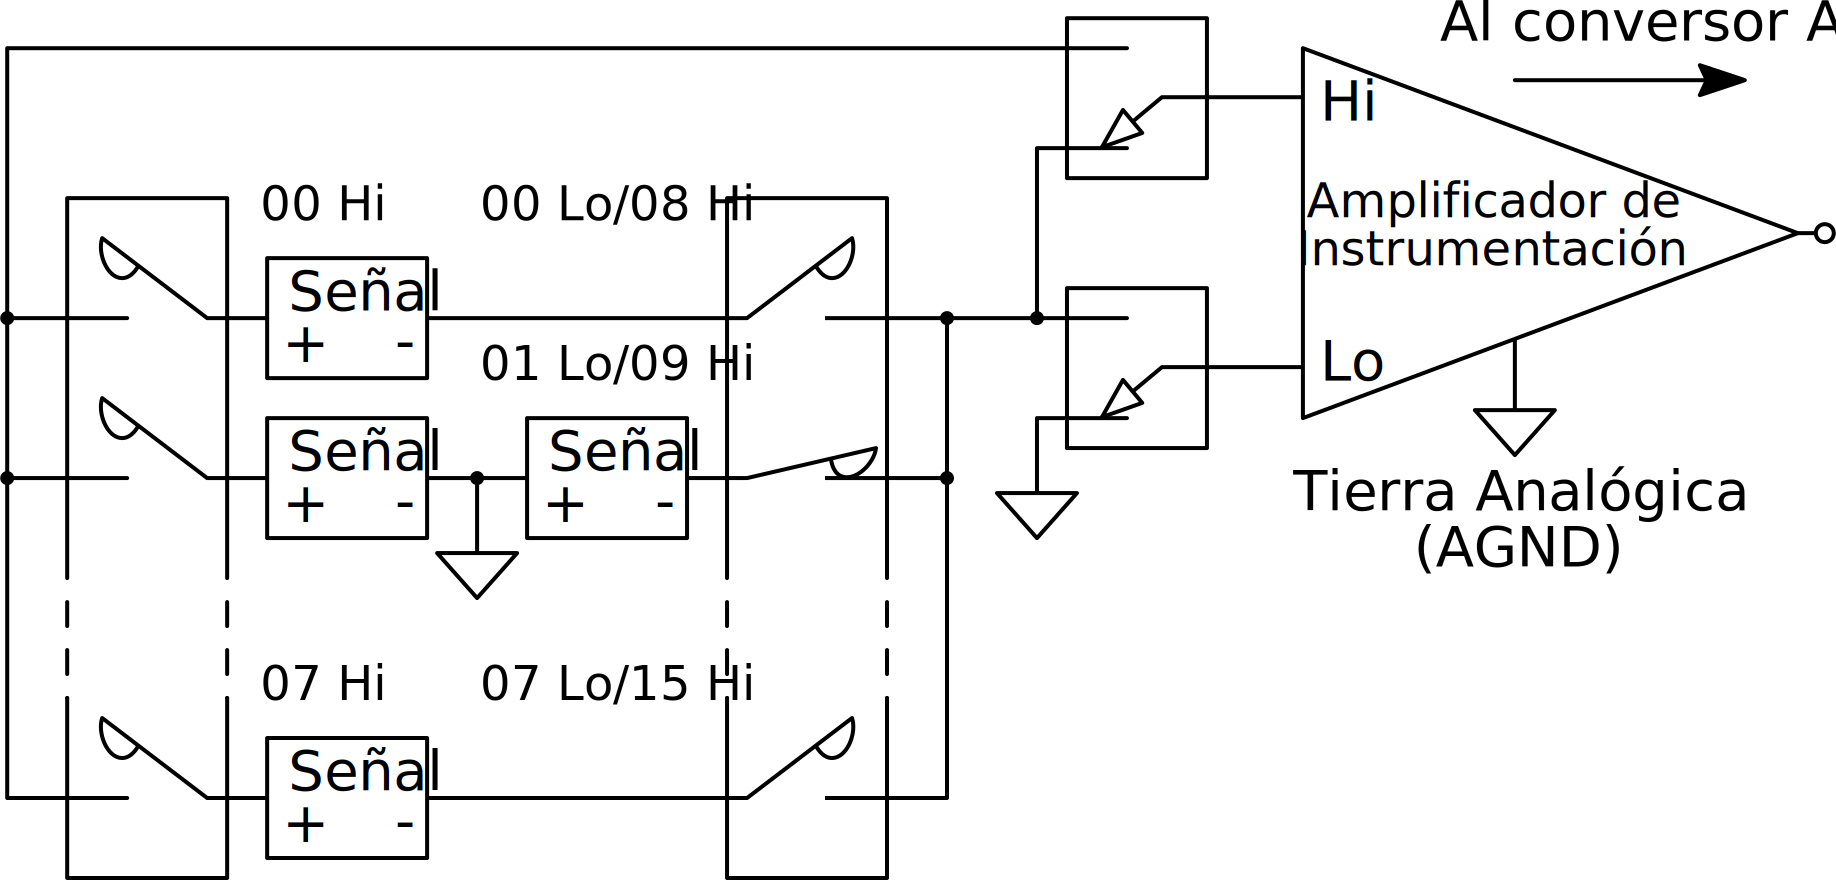
\includegraphics{gis-pfc-ch1-1.mps}
	\end{center}
	\caption[Ejemplo de configuraci�n de terminaci�n]{Figura que muestra el modo de terminaci�n sencillo. La entrada superior del amplificador de instrumentaci�n se conecta al puerto 9 y la entrada inferior se conecta a masa}
	\label{fig:termmodes}
\end{figure}

Para habilitar semejante configuraci�n, cabr�a pensar que es suficiente con modificar el atributo que controla el modo de terminaci�n del canal correspondiente. Al contrario de lo que pudiera parecer, el modo de terminaci�n es una propiedad que no es atribuible al canal, si no que se atribuye a un par de puertos\footnote{Aunque seg�n las especificaciones del fabricante es posible configurar cada par de puertos para que opere seg�n un modo de terminaci�n independiente del resto, el entorno de desarrollo utilizado durante el proyecto s�lo admite un modo de terminaci�n para el conjunto total de puertos (v. el \vref{subsec:environment}).}. En concreto, el modo de terminaci�n afecta a los pares de puertos compuestos por un primero de entre los puertos 0 y 7, y un segundo cuyo n�mero de puerto es igual al del primero m�s 8. De ah� que todos los canales relacionados con el mismo par de puertos deban estar configurados con el mismo modo de terminaci�n, una configuraci�n distinta no est� permitida.\par
Los dos modos de terminaci�n posibles se conocen como: diferencial, si es que la se�al que entra en cada terminal del amplificador procede de cada uno de los puertos del par; sencillo, en caso de que uno de los terminales de entrada del amplificador se conecte a la referencia de tensi�n. En este documento se llama canal diferencial a los canales cuyo modo de terminaci�n sea diferencial, y canal con un s�lo terminal o monoterminal a aquellos para los que el modo de terminaci�n es sencillo. \par
Las ventajas que presenta el uso de uno u otro tipo de canales son comprensibles. Emplear canales con un s�lo terminal permite aplicar el proceso de adquisici�n sobre un mayor n�mero de se�ales simult�neamente. Por el contrario, utilizar canales diferenciales redunda en una mayor inmunidad frente al ruido. Adem�s, los amplificadores diferenciales eliminan de forma inherente la componente en continua.\par


\subsection{Rendimiento}\label{subsec:throughput}

Se entiende como rendimiento la cantidad m�xima de operaciones de conversi�n que el dispositivo puede realizar por unidad de tiempo. Para que una de estas operaciones contribuya a la medida de rendimiento debe superar un requisito de precisi�n.\par
El rendimiento �ptimo de la tarjeta \kpci{} especificado por el fabricante es de cien mil operaciones por segundo (100 KS/s). No obstante se advierte, para obtener este nivel de rendimiento es necesario alimentar la tarjeta con una fuente de tensi�n ideal. Adem�s, es importante que exista adaptaci�n de impedancias entre el circuito de alimentaci�n y el puerto por el que se quiere introducir la se�al. A�n en estas condiciones el valor proporcionado por la casa Keithley est� sujeto a un error relativo m�ximo del $0.02\%$, el cual supone un error absoluto m�ximo de dos mil operaciones por segundo (2 KS/s).\par
Es bien sabido, a trav�s del teorema de Nyquist, que la frecuencia de muestreo con la que debe muestrearse una se�al anal�gica para que esta pueda ser recuperada a partir de la versi�n digital obtenida en el proceso de muestreo debe ser mayor o igual al doble de la mayor de las frecuencias con las que oscila la se�al original, siempre que esta sea peri�dica y se encuentre limitada en banda. No obstante, en la pr�ctica, para poder elaborar una representaci�n visual aceptable de se�ales que no se encuentren sujetas a tales limitaciones ---ancho de banda finito y periodicidad de la se�al--- la frecuencia de muestreo debe estar en torno a unas cinco veces el l�mite superior de frecuencias correspondiente a la se�al que desea representarse. Por este motivo el rendimiento del dispositivo de adquisici�n y por ende del sistema de adquisici�n y procesado que en �ste se sustenta es un factor limitante que determina la frecuencia de oscilaci�n m�xima de la se�ales con las que dicho sistema trabaja. En este caso, considerando el montaje propuesto para el desarrollo de los experimentos que ata�en a este proyecto, el rendimiento de la \kpci{} limita la frecuencia de operaci�n de los transductores empleados y, en consecuencia, la profundidad de penetraci�n de los pulsos ultras�nicos y, por consiguiente, el espesor m�ximo de las muestras empleadas en los experimentos. Esta relaci�n surge inequ�vocamente de las conclusiones que se extraen de los desarrollos llevados a cabo en este mismo documento en el \cref{subsec:field}, expuestas en parte en otro \nameref{subsec:quality}, el \vref{subsec:quality}.


\subsubsection[Factores limitantes del rendimiento]{Amplificador de instrumentaci�n y p�rdida del rendimiento}

El amplificador de instrumentaci�n interno de la \kpci{} es de ganancia variable. Es posible configurar una ganancia distinta para cada canal. El prop�sito del amplificador es permitir al usuario modificar la amplitud de la se�al que entra al conversor. La intenci�n que se persigue es conseguir que la conversi�n se enfoque en los detalles de la se�al que sean de mayor inter�s y se pierda la m�nima informaci�n posible. Todo ello a�n trabajando simult�neamente con m�ltiples se�ales cuyo rango de amplitudes es con frecuencia muy diferente.\par
La desventaja que presenta esta configuraci�n ---multiplexor, amplificador de instrumentaci�n, conversor--- es una p�rdida de rendimiento que se produce en situaciones determinadas a causa de la intervenci�n del amplificador en la operaci�n de adquisici�n.\par
Cada ciclo de reloj cambia el canal activo y debe cambiar, si es oportuno, la se�al que accede al amplificador. Este proceso no es inmediato. Tras conmutar el multiplexor que precede al amplificador, se da paso al puerto conveniente. No obstante, la se�al que recibe el amplificador presenta, hasta transcurrido un determinado periodo de tiempo, una componente residual de la se�al que se amplific� en el anterior ciclo de reloj. Transcurrido dicho periodo de tiempo la se�al que entra al amplificador se ve libre de esa componente residual y se corresponde �nicamente con la se�al que entrega el multiplexor, se dice que se ha fijado la se�al.\par
Y es as� como el amplificador es causa de p�rdida de rendimiento, por medio de las componentes residuales. Si la conversi�n se realiza antes de fijar la se�al, el conversor toma un valor de la se�al corrompido por la componente residual de la se�al precedente. Por tanto, la muestra resultante queda igualmente corrompida incluso hasta el punto de perder su validez. Las operaciones de conversi�n que tengan como resultado muestras inv�lidas s�lo contribuyen a falsear la medida de rendimiento, haciendo que parezca mayor de lo que en realidad es.\par
El fabricante da a entender que existe una soluci�n de dise�o que resuelve en parte el problema planteado por las componentes residuales. Esta soluci�n consiste en alargar de forma deliberada la duraci�n del ciclo de reloj, de esa forma se proporciona tiempo suficiente para fijar la se�al. Sin embargo, esta soluci�n presenta dos inconvenientes: no solventa el problema en la totalidad de los casos y es, asimismo, una forma de perder rendimiento. Lo cual conduce inevitablemente a una soluci�n de compromiso, alargar el ciclo de reloj lo suficiente para que en la mayor�a de los casos el efecto de las componentes residuales sobre la precisi�n de la conversi�n no invalide las muestras resultantes y se produzca, por tanto, una ca�da del rendimiento, sin que la duraci�n del nuevo ciclo contribuya por s� misma a una p�rdida notable de �ste.\par


\subsubsection{Optimizaci�n del rendimiento}

Como se ha visto, la inclusi�n del amplificador en el dise�o de la tarjeta es causa directa o indirecta de una p�rdida de rendimiento. La magnitud de esa ca�da en el rendimiento depende de la configuraci�n de la cola de muestreo y de la amplitud de la se�al una vez llega �sta al dispositivo de adquisici�n.

\begin{itemize}
	\item Las se�ales cuya tensi�n absoluta se encuentra por debajo de los 100 mV al llegar a la \kpci{} sufren en mayor medida las consecuencias del empleo de un amplificador en la operaci�n de conversi�n. En primer lugar la se�al tarda m�s en fijarse de modo que el rendimiento se reduce a la mitad en las mejores condiciones, de 100 KS/s pasa a 50 KS/s. Esto es debido a que, al ser la amplitud de la se�al y la del ruido comparables, especialmente despu�s de que �ste se vea reforzado por el efecto de las componentes residuales, se genera una mayor incertidumbre.\par
	Por otro lado las se�ales que requieren que el amplificador opere con alta ganancia son las m�s perjudicadas por los problemas que causa el amplificador en configuraciones multiganancia, tal y como se explica a continuaci�n.
	\item Por lo general, el rendimiento se ve afectado de forma m�s pronunciada por el efecto de las componentes residuales en configuraciones multiganancia en las que se encadenan secuencias de canales con ganancia diferente. Una configuraci�n multiganancia de la cola de muestreo implica que en diferentes ciclos de reloj el amplificador act�a con ganancias distintas. Eso con frecuencia significa que el rango en el que se encuentra comprendida la amplitud de las se�ales que est�n entrando al dispositivo de adquisici�n es diferente de una se�al a otra. Cuando as� ocurre puede sucederse en ocasiones que en ciclos de reloj consecutivos entren al amplificador dos se�ales de amplitud diferente, siendo la amplitud de la se�al que ocupa el primer ciclo mucho mayor que la de la otra se�al en el tiempo en el que ambas permanecen a la entrada del dispositivo. Por otro lado, parece l�gico considerar que la componente residual asociada a una se�al cuya amplitud sea predominantemente mayor que la de otra se�al es de mayor amplitud inicial y mayor duraci�n temporal que la asociada a la segunda se�al. Por tanto si ocurre como se ha dicho y se tiene en cuenta la base probable que se ha propuesto, cuando la segunda de las se�ales se convierte en la se�al activa la amplitud de la componente residual asociada a la primera de ellas puede ser suficiente, incluso, para enmascararla.\par No s�lo eso, la amplitud de la se�al que llega m�s tarde al amplificador puede ser, en t�rminos absolutos, la mayor parte del tiempo, menor que la de la otra se�al, al ser as� lo m�s probable es que se amplifique empleando un mayor factor de ganancia. De ser as�, la amplitud de la componente residual a la que se enfrenta esta se�al puede provocar en el peor de los casos que el conversor sature y la p�rdida de precisi�n sea mucho mayor. Sea cual sea el caso, es posible observar entonces, que en configuraciones multiganancia las muestras resultantes se obtienen de una conversi�n menos precisa, en especial si se trabaja con se�ales de peque�a amplitud ---tal y como se especific� en el punto anterior--- o si las ganancias configuradas en la cola de muestreo difieren mucho unas de otras. Aplicando la relaci�n entre la validez de las muestras y el rendimiento de la que se habl� anteriormente, la consecuencia de emplear configuraciones multiganancia es una mayor p�rdida de rendimiento.
	\item En configuraciones monoganancia el uso del amplificador supone una causa indirecta de la ca�da de rendimiento. El dise�o del dispositivo de adquisici�n est� pensado primordialmente para su uso en configuraciones multiganancia, de lo contrario la inclusi�n de un amplificador de ganancia variable en el esquem�tico de la tarjeta ser�a incomprensible. Por la misma raz�n, Keithley adopta una soluci�n de dise�o como la expuesta en el anterior apartado, para tratar de obtener un rendimiento �ptimo en configuraciones multiganancia. Sin embargo, el efecto de las componentes residuales en configuraciones monoganancia es m�nimo y la consecuente p�rdida de rendimiento tambi�n lo es. Por tanto, una soluci�n que consiste en alargar el ciclo de reloj resulta, en configuraciones monoganancia, innecesaria y perjudicial para el rendimiento.
\end{itemize}

Las acciones que el fabricante adopta para tratar de que el usuario obtenga el mayor rendimiento posible del dispositivo no se limitan a aplicar una soluci�n de compromiso en el dise�o de la duraci�n del ciclo de reloj. En el manual de usuario se hacen una serie de recomendaciones de uso orientadas a conseguir este fin.\par
Se proponen varias soluciones, la m�s trivial de las cuales pasa por preamplificar todas las se�ales que vayan a ser objeto del proceso de adquisici�n efectuado por la tarjeta consiguiendo que su amplitud var�e en un mismo rango. Si se hace as�, es suficiente con emplear una configuraci�n monoganancia para minimizar los efectos de las componentes residuales en el rendimiento. Adem�s al preamplificar las se�ales, �stas presentan una mejor relaci�n se�al a ruido, es decir, son menos vulnerables al ruido. Aunque buena, esta soluci�n no deja de ser trivial puesto que el amplificador de instrumentaci�n de la tarjeta pierde toda funcionalidad y pasa a ser un estorbo en el proceso de adquisici�n.\par
La soluci�n de car�cter pr�ctico propuesta por Keithley radica configurar la cola de muestreo de forma minuciosa, persiguiendo optimizar el rendimiento. Como se ha visto, en determinadas ocasiones una configuraci�n inapropiada de la cola de muestreo puede inducir que la p�rdida de productividad que provoca la inclusi�n del amplificador en el circuito de adquisici�n sea todav�a mayor. Para evitar que esto ocurra y sacar el m�ximo partido del dispositivo se dan en el manual dos condiciones que de cumplirse garantizan que la cola se encuentre configurada de forma �ptima en t�rminos de rendimiento.

\begin{itemize}
	\item La primera consiste en agrupar canales con distinta ganancia en posiciones consecutivas de la cola, a�n si al hacerlo se pierde el orden de muestreo definido en una primera instancia por el usuario. Si como se presupuso en el apartado anterior, com�nmente dos se�ales que requieren ser amplificadas con el mismo factor de ganancia var�an en el mismo rango de amplitudes, en estas secuencias monoganancia las consecuencias de las componentes residuales en la precisi�n de la conversi�n son m�nimas.
	\item A pesar de emplear una configuraci�n como la anterior, la aparici�n de saltos de ganancia en la cola de muestreo es todav�a probable. Por ejemplo, en la transici�n entre dos secuencias monoganancia como las descritas arriba. El salto es a�n m�s problem�tico si la transici�n se realiza para dar paso a una secuencia de ganancia mayor. El primer canal de esta secuencia sufre en mayor proporci�n los efectos de las componentes residuales y el rendimiento asociado al canal se ve reducido dram�ticamente. Para minimizar el impacto que en determinados canales como �ste tienen los problemas causados por el amplificador, es posible modificar la configuraci�n de la cola para que dichos canales ocupen varias posiciones consecutivas. Esta segunda condici�n persigue dar m�s tiempo para que se fije la se�al cuando los mencionados canales est�n activos. Para ello se necesitan posiciones vac�as en la cola, posiciones que es posible obtener desalojando canales previamente configurados.
\end{itemize}


\section{Comunicaci�n con el perif�rico}

Para la interacci�n con dispositivos externos, la \kpci{} dispone de dos conectores formato mini-\sig{d} de 36 terminales que cumplen con el est�ndar \sig{ieee} 1284 de protocolos de comunicaci�n en paralelo. Si se observa la tarjeta como el rect�ngulo que forma desde un punto de vista geom�trico y observ�ndola de frente, los conectores quedan ubicados en un lado de la tarjeta contiguo a aquel en el que se sit�a la conexi�n \sig{pci}. Todo ello de forma que tras el montaje del perif�rico en la placa base los conectores quedan expuestos en la parte posterior de la carcasa en la que providencialmente debe encontrarse instalada dicha placa, tal y como es habitual en este tipo de dispositivos.\par
En la \cref{fig:ports} se etiqueta cada terminal seg�n su ubicaci�n relativa con respecto al conector y al resto de terminales en el mismo, para cada conector, mostrando la distribuci�n definida por el fabricante. Los \cref{tab:analog,tab:digital} describen el prop�sito de cada terminal y se especifica que tipo de se�al debe circular por los mismos.

\newbox{\portbox}
\sbox{\portbox}{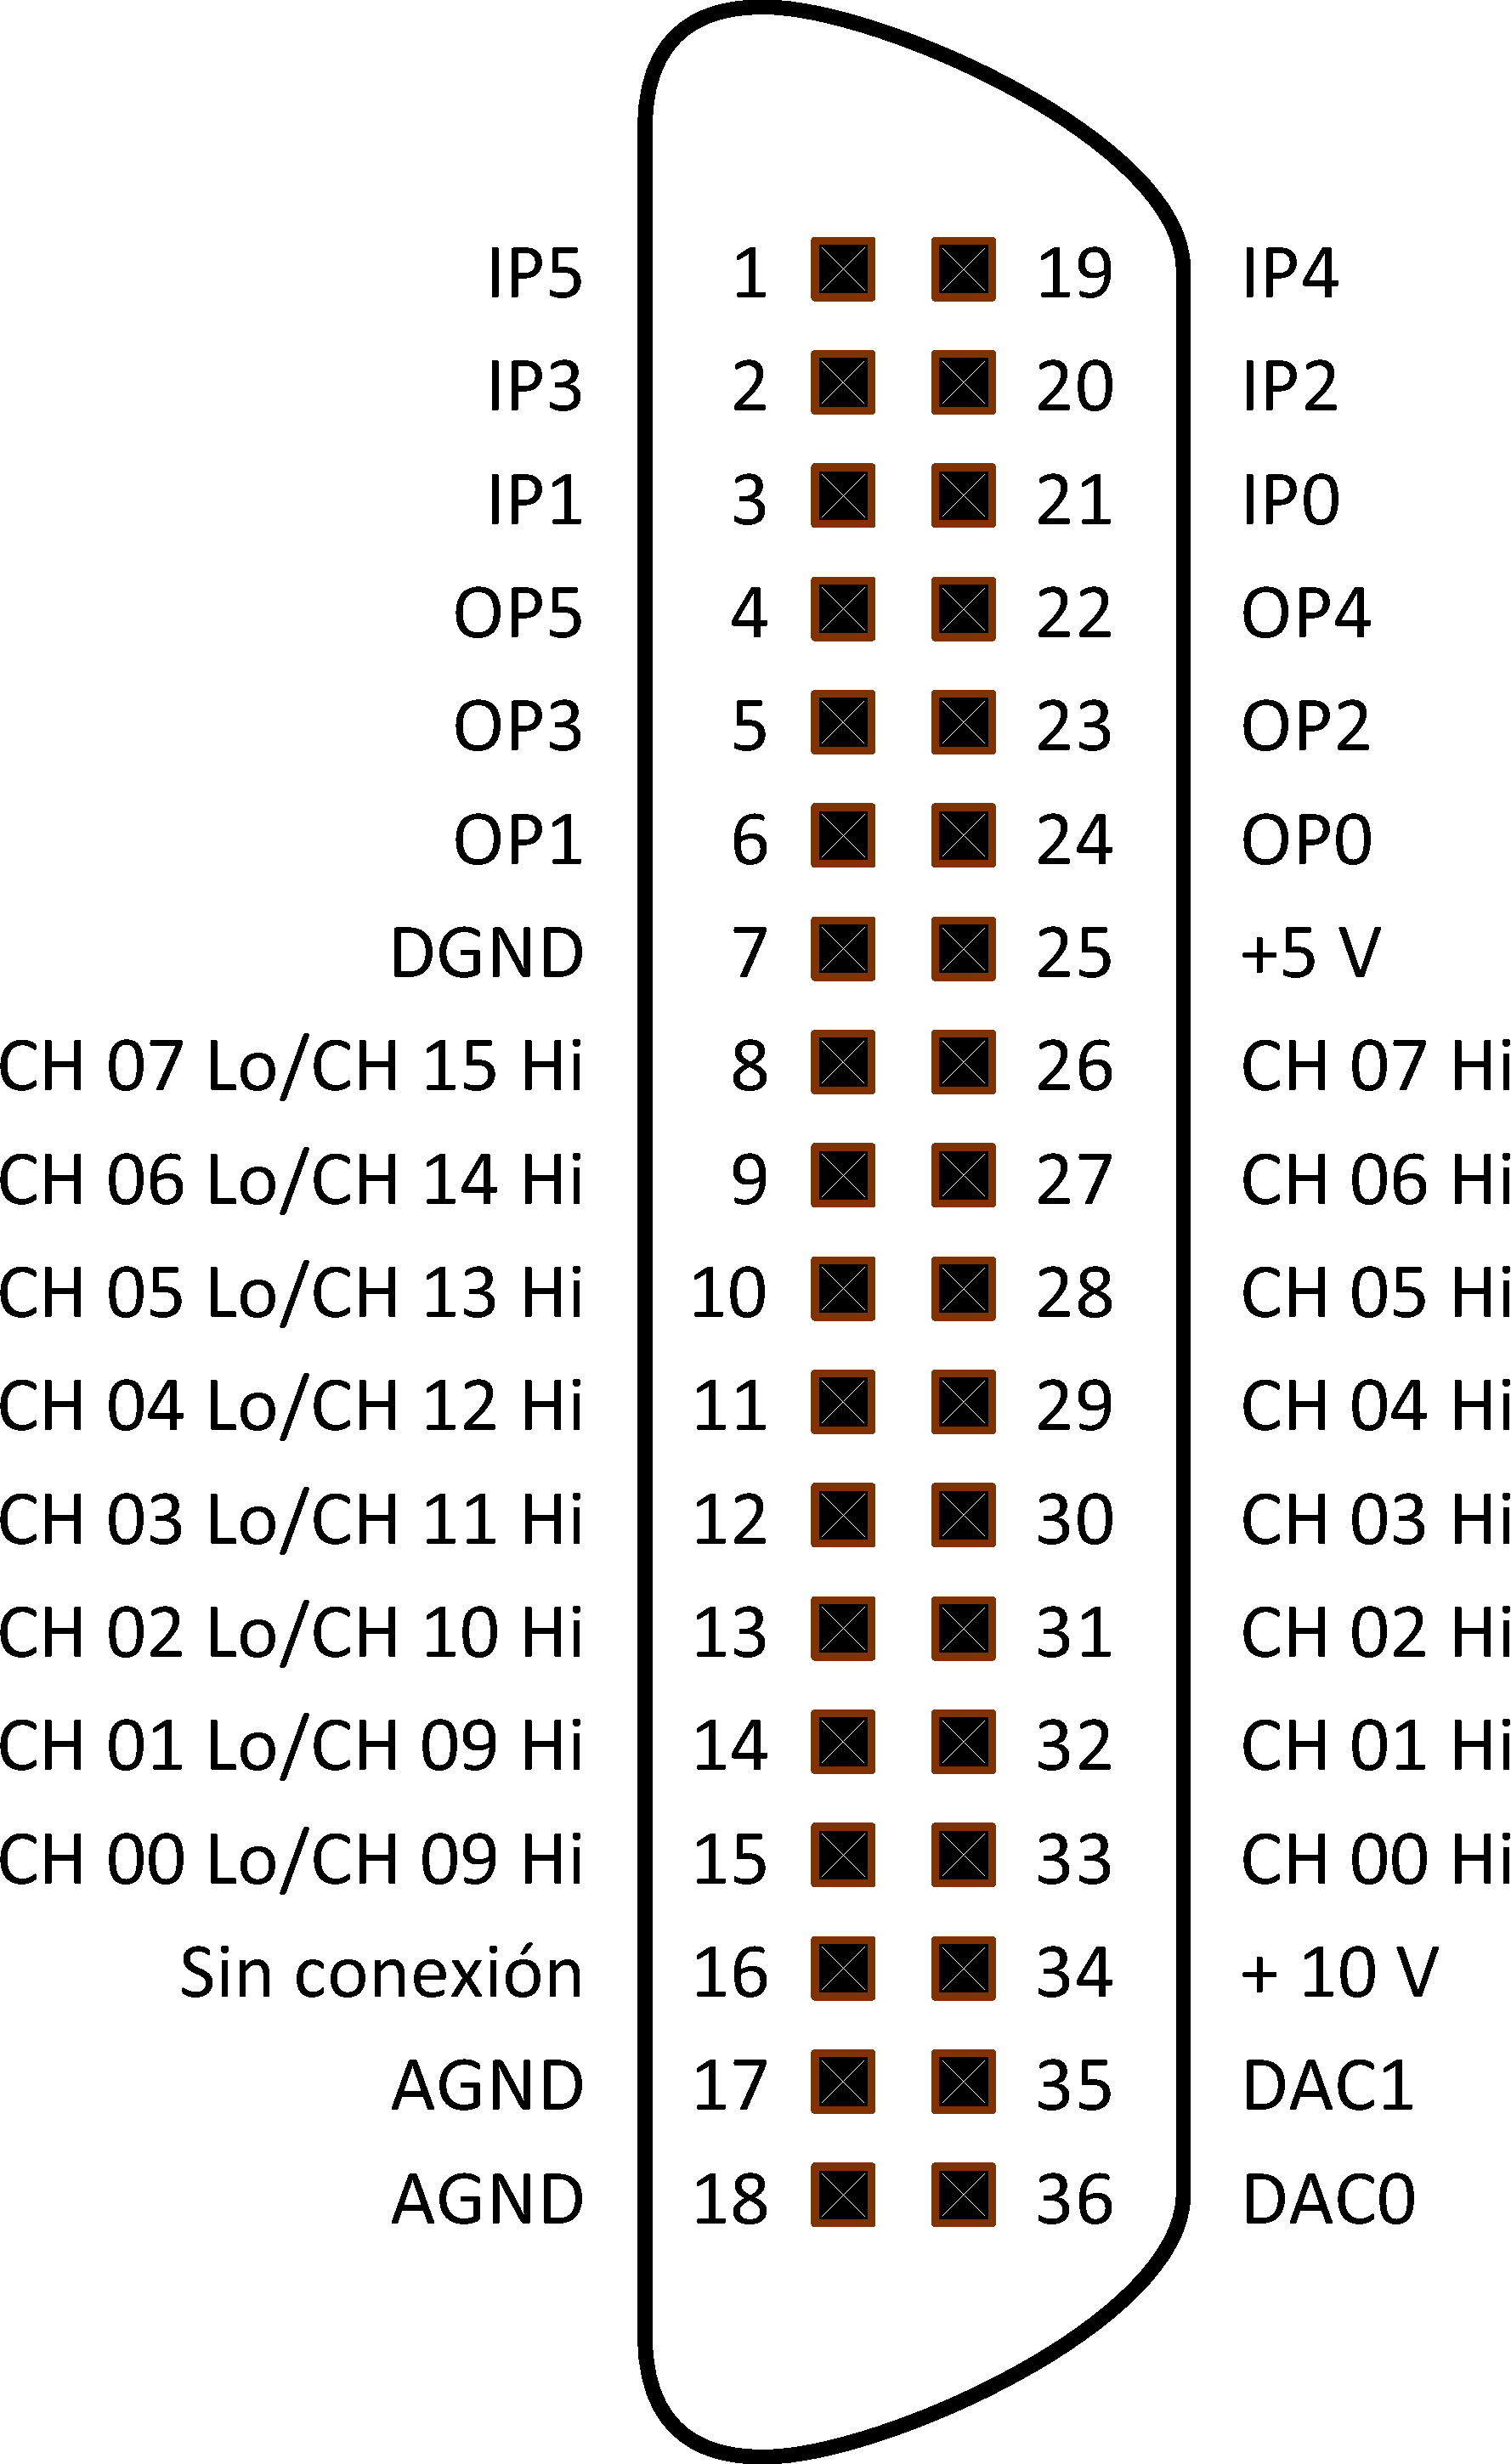
\includegraphics[width=.4\textwidth, keepaspectratio=true]{gis-pfc-ch1-2.pdf}}

\begin{figure}
	\centering
	\subfloat[Conector etiquetado como ``analog'']{%
		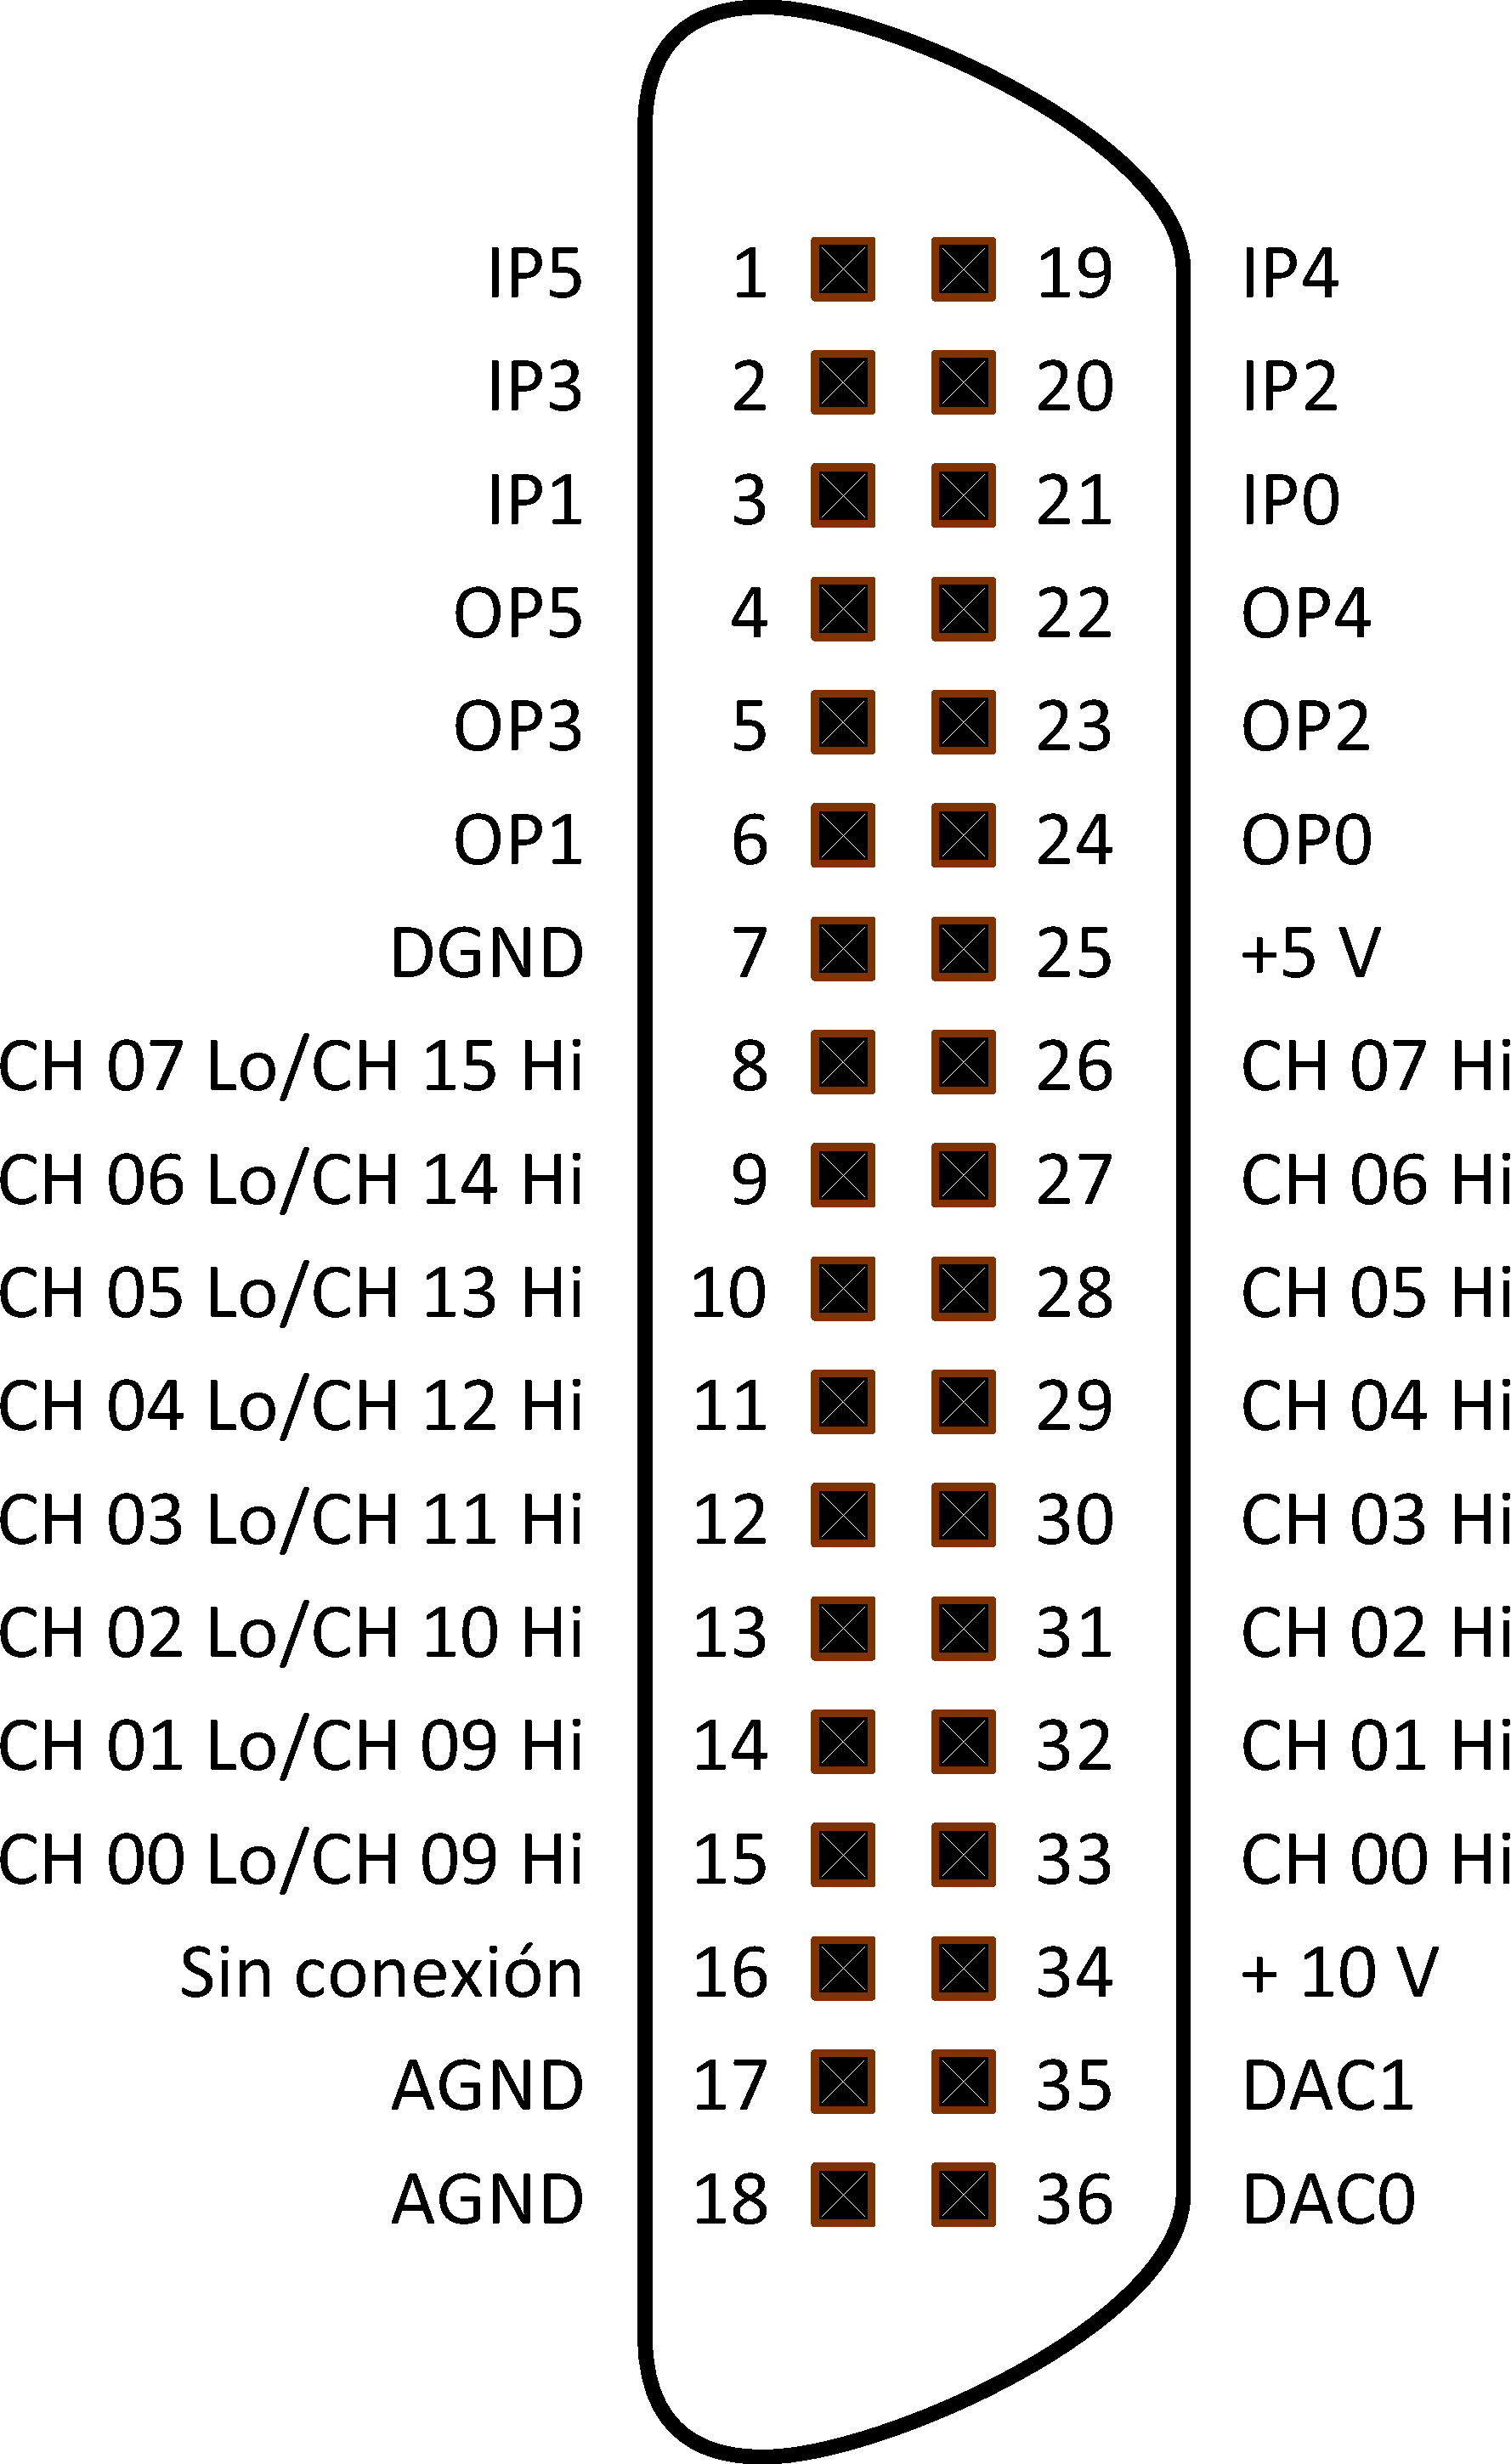
\includegraphics[width=.4\textwidth, keepaspectratio=true]{gis-pfc-ch1-2.pdf}}\qquad
	\subfloat[Conector etiquetado como ``digital'']{%
		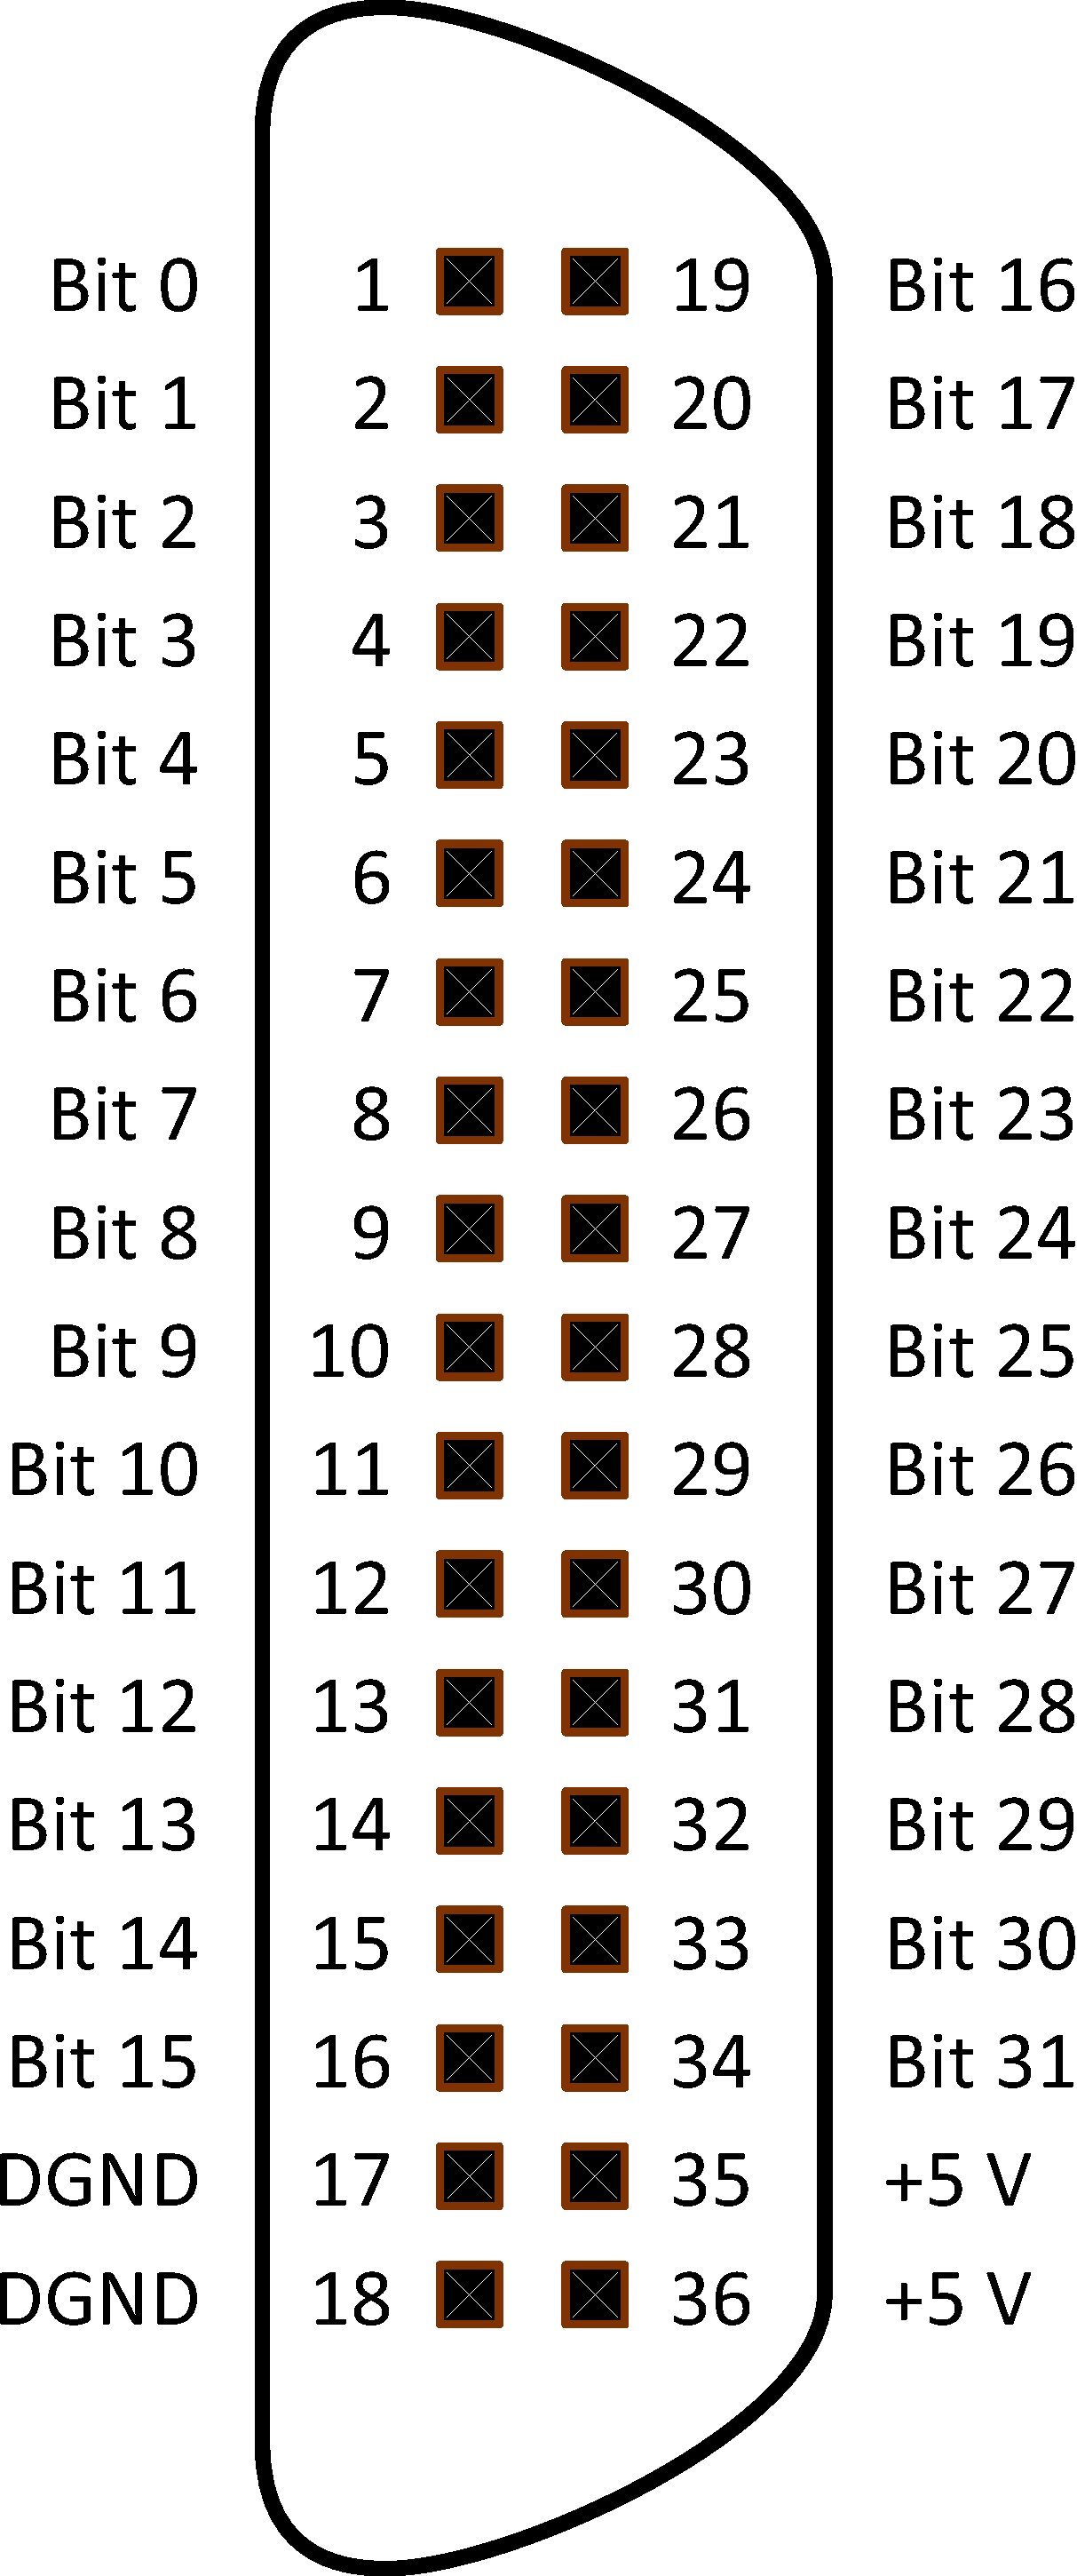
\includegraphics[height=\ht\portbox, keepaspectratio=true]{gis-pfc-ch1-3.pdf}}
 	\caption{Esquema del panel de conexiones trasero de la \kpci{}}
	\label{fig:ports}
\end{figure}


\begin{table}
	\centering
	\begin{tabular}{>{\raggedleft}p{1cm} >{\scshape}c >{\arraybackslash}l}
		\toprule
		\multicolumn{1}{c}{Terminal} & {\upshape Puerto asignado} & \multicolumn{1}{c}{Descripci�n} \\
		\midrule
		1 & ip5 & \multirow{12}{0.6\textwidth}{Bits digitales de entrada multifunci�n. Pueden ser configurados por el usuario para que ejerzan la funci�n de:\miniit{\item Base temporal para el contador/temporizador y/o entrada a \emph{gate} \\\item Reloj externo para conversiones A/D o D/A \\\item Disparador digital externo \\\item Entrada digital en el modo \emph{target-mode}}} \\
		2 & ip3 & \\
		3 & ip1 & \\
		\\\\\\\\\\\\\\\\
		\midrule
		4 & op5 & \multirow{12}{0.6\textwidth}{Bits digitales de salida multifunci�n. Pueden ser configurados por el usuario para que ejerzan la funci�n de:\miniit{\item Salidas del contador/temporizador\\\item Salida del disparador\\\item Salida de control para accesorios\\\item Salida del reloj interno\\\item Salida digital en el modo \emph{target-mode}}} \\
		5 & op3 & \\
		6 & op1 & \\
		\\\\\\\\\\\\\\\\
		\midrule
		7 & dgnd & \multicolumn{1}{c}{Tierra digital} \\
		\midrule
		8 & ch07 lo/ch15 & \multirow{4}{0.6\textwidth}{Entradas anal�gicas, cuya funci�n depende del modo de terminaci�n configurado: puerto asociado a un canal monoterminal o puerto bajo de un canal diferencial} \\
		9 & ch06 lo/ch14 & \\
		10 & ch05 lo/ch13 & \\
		$\vdots$ & $\vdots$ & \\
		15 & ch00 lo/ch08 & \\
		\midrule
		16 & {\upshape Sin conexi�n} & \\
		\midrule
		\multicolumn{1}{l}{17, 18} & agnd & Tierra anal�gica \\
		\bottomrule
	\end{tabular}
	\caption{Relaci�n entre los puertos y terminales que presenta el conector trasero de la \kpci{} etiquetado como \emph{analog}}
	\label{tab:analog}
\end{table}

\begin{table}\ContinuedFloat
	\centering
	\begin{tabular}{>{\raggedleft}p{1cm} >{\scshape}c >{\arraybackslash}l}
		\toprule
		\multicolumn{1}{c}{Terminal} & {\upshape Puerto asignado} & \multicolumn{1}{c}{Descripci�n} \\
		\midrule
		19 & ip4 & \multirow{12}{0.6\textwidth}{Bits digitales de entrada multifunci�n. Pueden ser configurados por el usuario para que ejerzan la funci�n de:\miniit{\item Base temporal para el contador/temporizador y/o entrada a \emph{gate} \\\item Reloj externo para conversiones A/D o D/A \\\item Disparador digital externo \\\item Entrada digital en el modo \emph{target-mode}}} \\
		20 & ip2 & \\
		21 & ip0 & \\
		\\\\\\\\\\\\\\\\
		\midrule
		22 & op4 & \multirow{12}{0.6\textwidth}{Bits digitales de salida multifunci�n. Pueden ser configurados por el usuario para que ejerzan la funci�n de:\miniit{\item Salidas del contador/temporizador\\\item Salida del disparador\\\item Salida de control para accesorios\\\item Salida del reloj interno\\\item Salida digital en el modo \emph{target-mode}}} \\
		22 & op2 & \\
		21 & op0 & \\
		\\\\\\\\\\\\\\\\
		\midrule
		25 & {\upshape +5 V} & \multirow{2}{0.6\textwidth}{Referencia de tensi�n de 5 voltios de corriente continua extra�dos del bus \sig{pci} del ordenador} \\
		& & \\
		\midrule
		26 & ch07 hi & \multirow{3}{0.6\textwidth}{Entradas anal�gicas restantes, en el modo de terminaci�n diferencial representan el puerto alto de un canal diferencial} \\
		27 & ch06 hi & \\
		28 & ch05 hi & \\
		$\vdots$ & $\vdots$ & \\
		33 & ch00 hi & \\
		\midrule
		34 & {\upshape +10 V} & \multirow{6}{.6\textwidth}{Entrada dise�ada para proporcionar al dispositivo una referencia externa de precisi�n de 10 voltios mediante una fuente de alta impedancia de salida (La impedancia de entrada de este puerto es equivalente a una resistencia de 1 k$\Omega$ en serie con la impedancia de entrada de la fuente)} \\
		\\\\\\\\\\
		\bottomrule
	\end{tabular}
	\caption[]{Continuaci�n del \vref{tab:analog}}
\end{table}

\begin{table}\ContinuedFloat
	\centering
	\begin{tabular}{>{\raggedleft}p{1cm} >{\scshape}c >{\arraybackslash}l}
		\toprule
		\multicolumn{1}{c}{Terminal} & {\upshape Puerto asignado} & \multicolumn{1}{c}{Descripci�n} \\
		\midrule
		35 & dac1 & \multirow{2}{.6\textwidth}{Salida n�mero 1 del conversor digital a anal�gico de la \kpci{}} \\
		\\
		\midrule
		36 & dac0 & \multirow{2}{.6\textwidth}{Salida n�mero 0 del conversor digital a anal�gico de la \kpci{}} \\
		\\
		\bottomrule
	\end{tabular}
	\caption[]{Continuaci�n del \vref{tab:analog}}
\end{table}

\begin{table}
	\centering
	\begin{tabular}{>{\raggedleft}p{1cm} >{\scshape}c >{\arraybackslash}l}
		\toprule
		\multicolumn{1}{c}{Terminal} & {\upshape Puerto asignado} & \multicolumn{1}{c}{Descripci�n} \\
		\midrule
		1 & {\upshape Bit 0} & \multirow{6}{0.6\textwidth}{Canal 0 de bits de entrada/salida de prop�sito general (En la \kpci{} los bits digitales se agrupan de en ocho en ocho en canales. Los canales de este tipo puede configurarse para que los bits que lo integran se comporten como todo salidas o todo entradas)} \\
		2 & {\upshape Bit 1} & \\
		3 & {\upshape Bit 2} & \\
		$\vdots$ & $\vdots$ & \\
		8 & {\upshape Bit 7} & \\
		\\
		\midrule
		9 & {\upshape Bit 8} & \multirow{2}{0.6\textwidth}{Canal 1 de bits de entrada/salida de prop�sito general} \\
		10 & {\upshape Bit 9} & \\
		11 & {\upshape Bit 10} & \\
		$\vdots$ & $\vdots$ & \\
		16 & {\upshape Bit 15} & \\
		\midrule
		\multicolumn{1}{l}{17, 18} & dgnd & Tierras digitales \\
		\midrule
		19 & {\upshape Bit 16} & \multirow{2}{0.6\textwidth}{Canal 2 de bits de entrada/salida de prop�sito general} \\
		20 & {\upshape Bit 17} & \\
		21 & {\upshape Bit 18} & \\
		$\vdots$ & $\vdots$ & \\
		26 & {\upshape Bit 23} & \\
		\midrule
		27 & {\upshape Bit 24} & \multirow{2}{0.6\textwidth}{Canal 3 de bits de entrada/salida de prop�sito general} \\
		28 & {\upshape Bit 25} & \\
		29 & {\upshape Bit 26} & \\
		$\vdots$ & $\vdots$ & \\
		34 & {\upshape Bit 31} & \\
		\midrule
		\multicolumn{1}{l}{35, 36} & {\upshape +5 V} & +5 V\sig{dc} desde el bus del ordenador \\
		\bottomrule
	\end{tabular}
	\caption{Relaci�n entre los puertos y terminales que presenta el conector trasero de la \kpci{} etiquetado como \emph{digital}}
	\label{tab:digital}
\end{table}


\subsection{Desarrollo de una nueva interfaz}\label{subsec:conbox}

Por razones pr�cticas, la interfaz original de la \kpci{} basada en dos conectores mini-\sig{d} no se acomoda a las necesidades que se prev� surgir�n durante el desarrollo de las pruebas requeridas para la finalizaci�n de este proyecto de fin de carrera. En consecuencia, con el prop�sito de agilizar en la medida de lo posible la realizaci�n de estos ensayos, se decide ampliar la interfaz existente.\par
Para ello se parte de dos extremos de cable terminados en un conector tipo macho y desprovistos de cubierta, de cada uno de los cuales surgen 36 hilos de cobre recubiertos de pl�stico flexible coloreado. El patr�n de coloreado de las cubiertas individuales es �nico y no se repite en ninguno de los 36 hilos de que se compone cada extremo de cable. A partir de ah�, se identifica cada terminal de cada conector con el hilo de cobre correspondiente, relacionando las etiquetas que el fabricante pone a los terminales con el c�digo de colores de la cubiertas individuales.\par
Una vez recopilada esta informaci�n, se planea la construcci�n de una caja de conexiones. El dise�o de la caja contempla que se equipe �sta con 72 conectores banana hembra soldados a los 72 hilos de cobre y que comunican con los terminales de los conectores mini-\sig{d} en los que termina el otro extremo de los cables. Adem�s se planifica la inclusi�n de cuatro conectores coaxiales con rosca con conexiones redundantes a las que se presupone son las cuatro puertas cuyo uso ser� m�s frecuente, las correspondientes al primer canal anal�gico diferencial y las tierras anal�gicas; para as� facilitar el uso continuado de las mismas. Por �ltimo se decide etiquetar la caja de conexiones con marbetes que reproduzcan la nomenclatura visible en la \vref{fig:ports}.\par
Puede observarse una representaci�n de la caja de conexiones ya terminada en la \vref{fig:conbox}.

\begin{figure}
	\begin{center}
		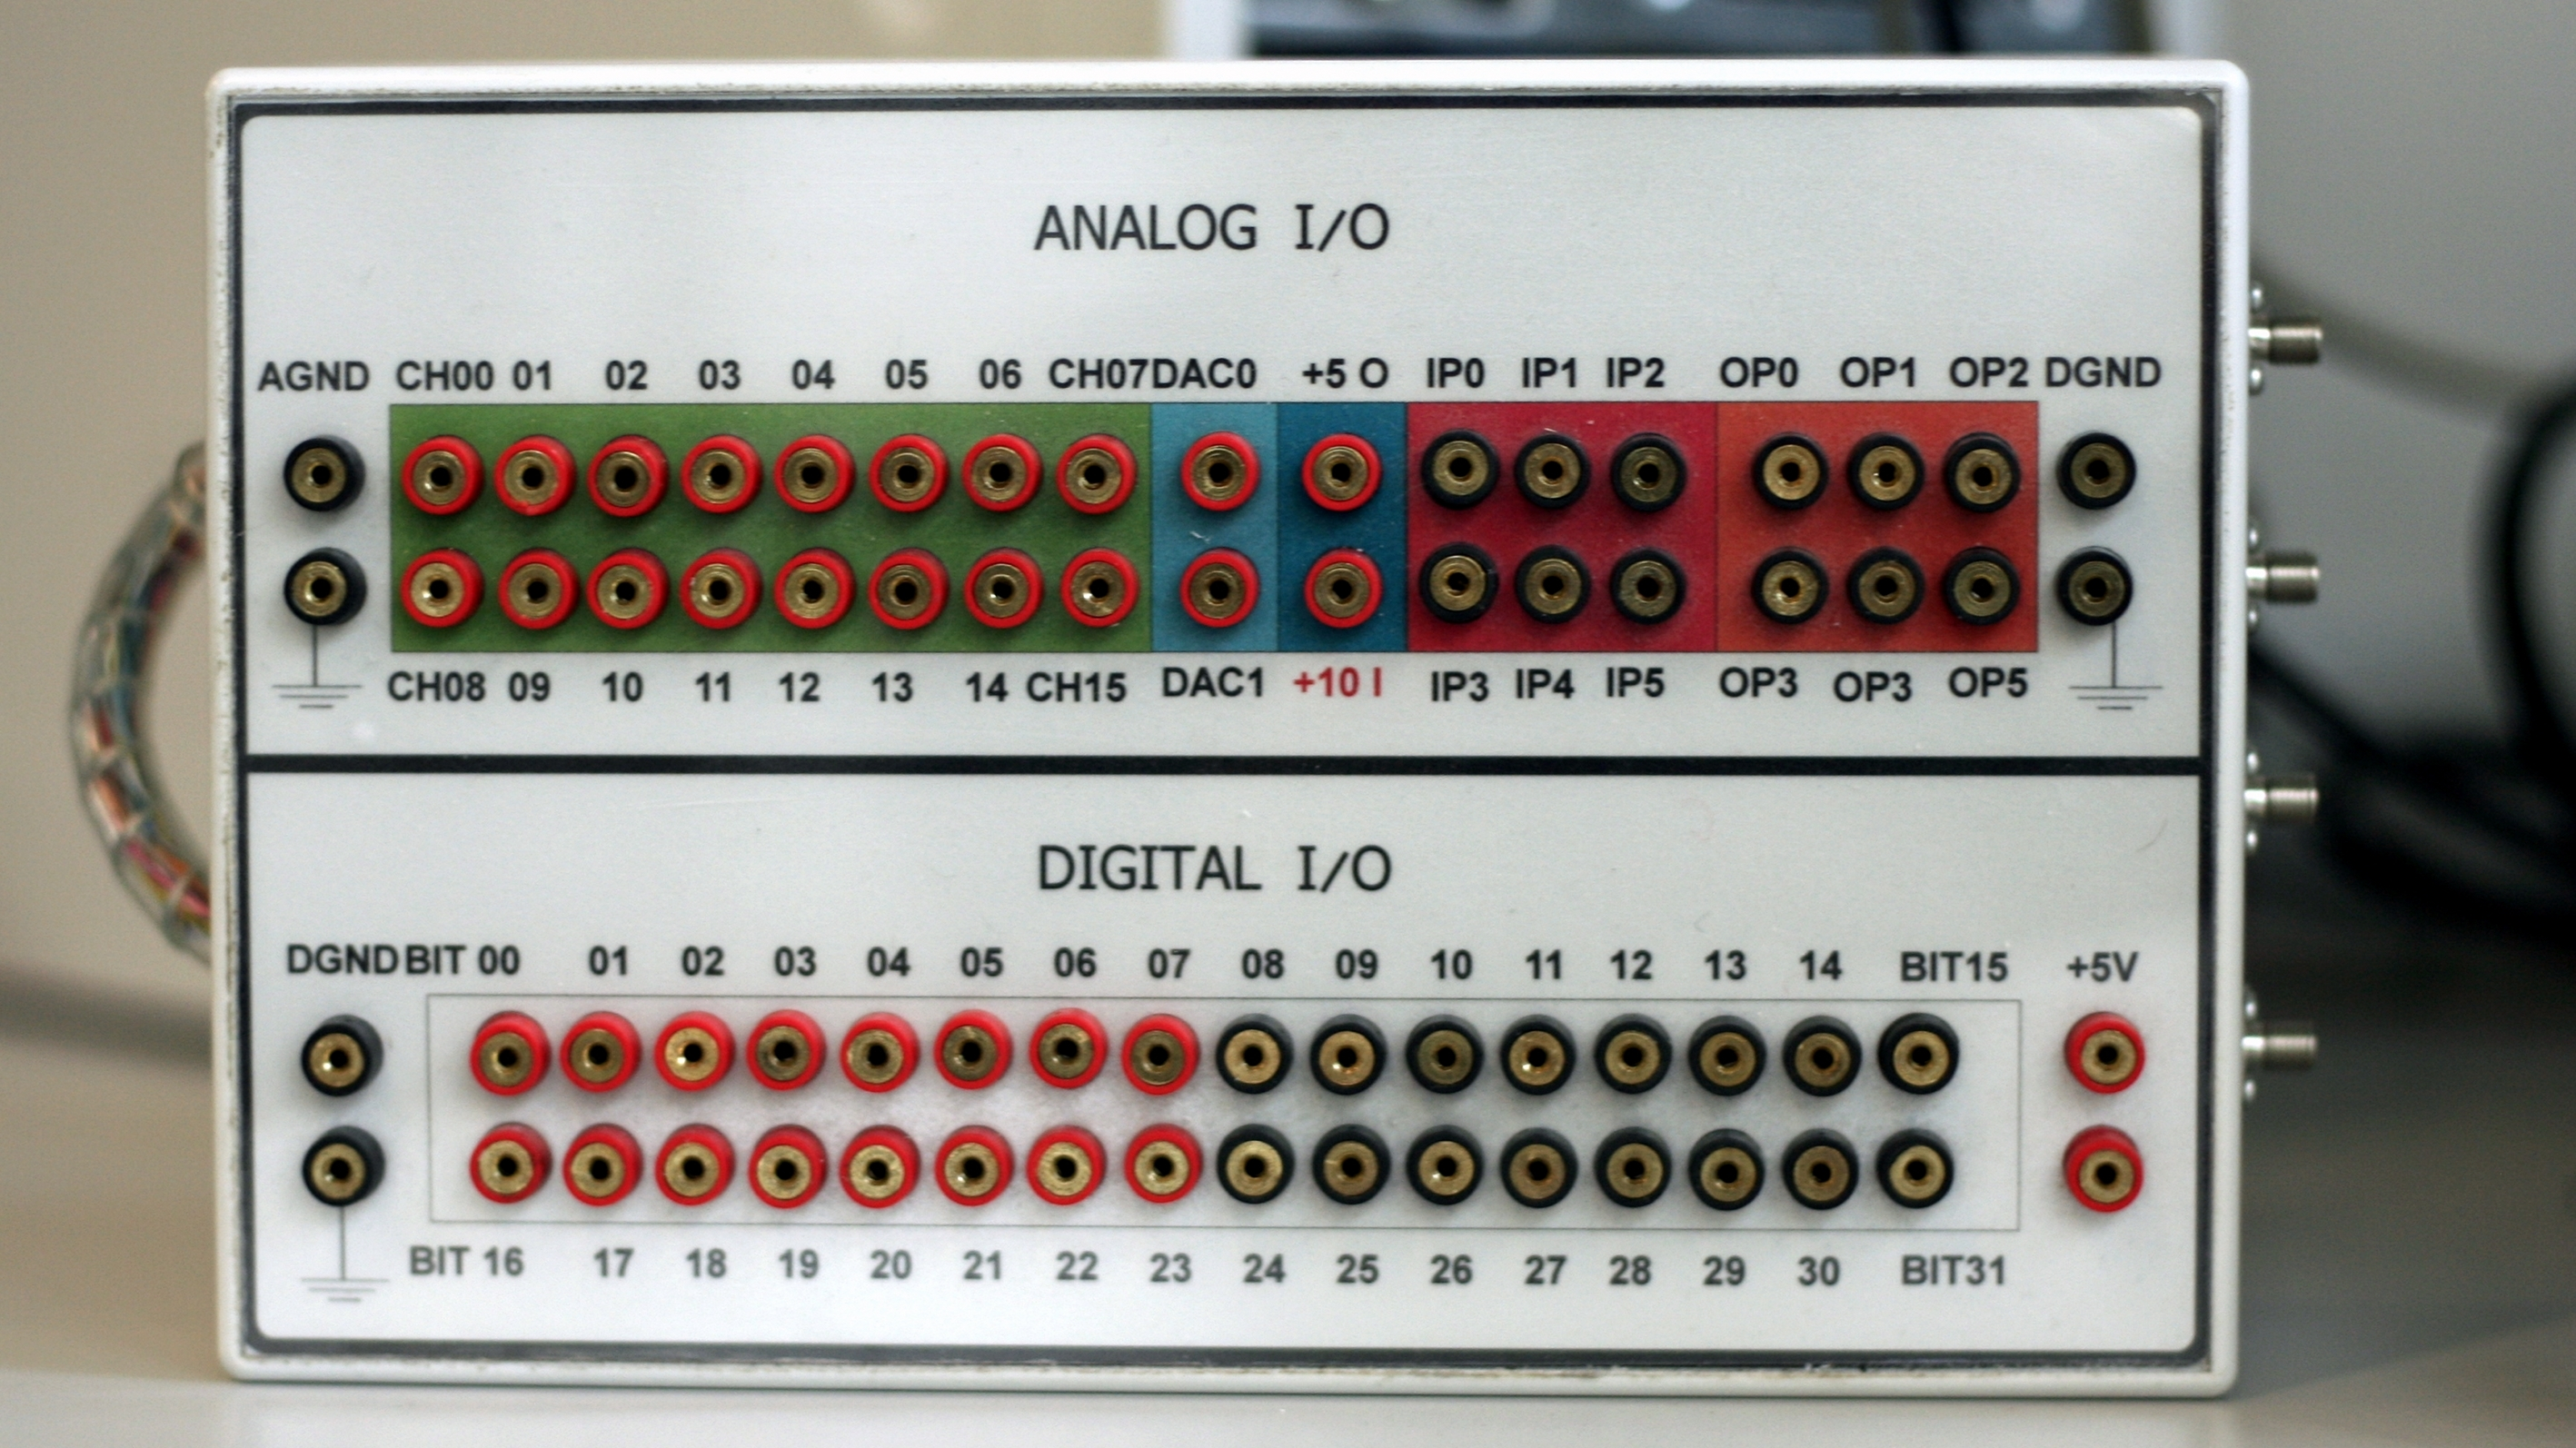
\includegraphics[scale=1, keepaspectratio=true]{gis-pfc-ch1-4.jpg}
	\end{center}
	\caption{Plano de la caja de conexiones ya terminada}
	\label{fig:conbox}
\end{figure}


\chapter{Subsistema de adquisición}

El subsistema de adquisición es el encargado de recibir la señal analógica
procedente del subsistema para la interacción con el medio físico,
muestrearla y proporcionar a las capas superiores una versión digital de la
misma. Es un subsistema exclusivo, y al mismo tiempo distintivo de los
sistemas digitales de medida. En la \cref{fig:subacqui} se muestra una
ventana parcial del sistema de medida digital centrada en las unidades
funcionales que conforman el subsistema de adquisición.

\begin{figure}
	\begin{center}
		\includegraphics{gis-pfc-ch2-01.mps}
	\end{center}
	\caption[Subsistema de adquisición] {Elementos funcionales que
	incluye el subsistema de adquisición.}
	\label{fig:subacqui}
\end{figure}

El subsistema de adquisición del sistema digital de medida propuesto para
el proyecto comprende un único bloque, un bloque de adquisición en el que
se ubica una tarjeta de adquisición. La tarjeta \kpci{} es el fundamento en
el que se basa, no sólo el subsistema de adquisición, si no el sistema
digital de medida al completo. Sus capacidades y muchas de sus limitaciones
las hereda el sistema, y constituyen los principios de diseño del resto de
subsistemas. El subsistema para la interacción con el medio debe proveer al
subsistema de adquisición con una señal que se ajuste a las
especificaciones de la tarjeta, además el circuito acondicionador de
recepción debe adaptar la impedancia de entrada mostrada por el
dispositivo. Por su parte, el subsistema de control y presentación debe ser
capaz de gestionar el funcionamiento de este instrumento y administrar los
valores de señal que proporciona. Además, la \kpci{}, disponer de ella, es
una de las razones principales por las que se ha optado por desarrollar un
sistema de adquisición propio, de propósito, sin tener en cuenta las
principales razones, como es obvio, uno de los objetivos del proyecto,
adquirir conocimientos prácticos en el campo del tratamiento digital de
señales y, por supuesto, contar con un sistema diseñado a medida. Por todas
estas razones, resulta comprensible realizar un estudio previo acerca de
las propiedades y el comportamiento de un instrumento de tan singular
importancia para este proyecto.

Esta memoria dedica un capítulo completo a exponer las características de
la tarjeta \kpci{}. Una breve relación de las características técnicas del
hardware da paso a la descripción funcional, en la que se explica cual es
el comportamiento interno de la tarjeta, como se implementan las distintas
funciones que ofrece. Para terminar el capítulo se reproducen los consejos
que el fabricante proporciona en el manual de usuario con la premisa de que
los usuarios consigan el máximo rendimiento de la tarjeta (punto
\ref{sec:throughput} en la página \pageref{sec:throughput}) y se muestra la
caja de conexiones elaborada expresamente para este proyecto.


\section{Características técnicas del hardware}\label{sec:technical}

La tarjeta \kpci{} puede emplearse para la adquisición y conversión de
señales analógicas en señales digitales, para sintetizar señales analógicas
a partir de señales digitales previamente generadas o almacenadas, o
---gracias a sus 32 puertos digitales de propósito general--- trabajar con
señales digitales.

El subsistema de adquisición dentro del sistema de medida digital requiere
únicamente de la función de adquisición analógica de la tarjeta. Por ello,
de entre todas las características del dispositivo, se ha creído
conveniente resumir a continuación aquellas que tienen relación directa con
dicha función. Para obtener información detallada sobre la relación que
estos atributos guardan con el proceso de adquisición de señales analógicas
en la tarjeta \kpci{}, véase la \vref{sec:funcdesc}.

\begin{itemize}
	\item El módulo de adquisición analógica dispone de 16 puertos
		físicos.
	\item La impedancia de entrada equivalente de cada puerto es
		aproximadamente igual a una capacidad de 200 pF en serie
		con una resistencia de valor inferior, pero aproximadamente
		igual, a 1 k$\Omega$.
	\item En condiciones óptimas, es posible conseguir un rendimiento
		máximo de 100 \kms{} (cien mil operaciones de conversión
		por segundo). Este valor está sujeto a un error relativo
		del $0.02\%$.
	\item La resolución del conversor analógico digital es de 16 bits
		por muestra. El rango de amplitudes en el que opera depende
		de como esté configurado el modo de adquisición. Puede ir
		de 0 V a 10 V si el modo de adquisición es unipolar, o de
		-10 V a 10 V si es bipolar.
	\item La cola de muestreo tiene capacidad para hasta 256 canales
		distintos. Cada uno de los cuales puede configurarse
		independientemente en términos de ganancia, frecuencia de
		muestreo, modo de adquisición o modo de terminación.
	\item La ganancia, responsable en parte de la resolución con la que
		se cuantifica las muestras, puede tomar cada ciclo de reloj
		uno de entre 16 valores posibles (véase el
		\vref{tab:acqmodes}).
\end{itemize}


\section{Descripción funcional}\label{sec:funcdesc}

Es necesario programar el comportamiento de la tarjeta de adquisición antes
de ponerla en funcionamiento. Desde la cola de muestreo se controlan los
principales aspectos del proceso de adquisición, como por ejemplo, en que
instantes se encuentra activo.

La cola de muestreo, como su propio nombre indica, es una estructura de
datos ordenada. Se encuentra almacenada en una memoria \sig{ram} de 256
entradas que forma parte del hardware de la tarjeta. En el \cref{tab:queue}
puede verse una representación de un ejemplo de la cola de muestreo.

\begin{table}
	\centering
	\begin{threeparttable}
	\begin{tabular}{lccccccccc}
		\toprule
		Posición en la cola & 1 & 2 & 3 & 4 %
		& \multicolumn{2}{c}{$\cdots$} & 254 & 255 & 256 \\
		\midrule
		Número de canal & 15 & 15 & 02 & 02 %
		& \multicolumn{2}{c}{$\cdots$} & 17 & 13 & 01 \\
		Número de puerto & 07 & 07 & 11 & 11 %
		& \multicolumn{2}{c}{$\cdots$} & 07 & 09 & 01 \\
		Ganancia & 1 & 1 & 40 & 40 %
		& \multicolumn{2}{c}{$\cdots$} & 200 & 8 & 80 \\
		Modo de adquisición\tnote{a} & $\pm$ & $\pm$ & $+$ & $+$ %
		& \multicolumn{2}{c}{$\cdots$} & $\pm$ & $+$ & $\pm$ \\
		Modo de terminación\tnote{b} & \sig{d} & \sig{d} %
		& \sig{m} & \sig{m} & \multicolumn{2}{c}{$\cdots$} %
		& \sig{d} & \sig{m} & \sig{m}\\
		\bottomrule
	\end{tabular}
	\begin{TableNotes}
		\tnotetext{a}{Configuración bipolar ($\pm$), configuración
		unipolar ($+$).}
		\tnotetext{b}{Canal diferencial (\sig{d}), canal
		monoterminal (\sig{m}).}
	\end{TableNotes}
	\end{threeparttable}
	\caption[Ejemplo de cola de muestreo]{Ejemplo de cola de muestreo.}
	\label{tab:queue}
\end{table}

Cada entrada en la memoria \sig{ram} se identifica con una posición en la
cola. Las posiciones en la cola pueden encontrarse vacías o estar ocupadas
por un canal. Varias posiciones en la cola, consecutivas o no, pueden estar
ocupadas por un mismo canal. Por tanto, la cola puede estar ocupada, como
máximo, por 256 canales independientes.

Las posiciones ocupadas contienen información correspondiente al canal y a
los atributos asociados a este. Un canal es una entidad lógica que
relaciona un puerto físico con un búffer de información y una serie de
atributos. Durante el proceso de adquisición un puntero recorre las
distintas posiciones de la cola, una a una y en orden. El canal activo,
aquel que ocupa la posición a la que apunta el puntero en cada ciclo de
reloj, determina tres cosas:

\begin{itemize}
	\item De qué puerto debe proceder la señal analógica\footnote{Por
		convenio se ha elegido hablar de una sola señal que entra
		al amplificador. Si se ha hecho esta elección, es porque si
		bien al amplificador pueden entrar una o dos señales
		simultáneamente, esto no supone otra diferencia para el
		proceso que la expuesta en el \vref{subsubsec:termmodes}.
		Es por ello, y para mantener la claridad, que se ha omitido
		esta posibilidad.} que llega al amplificador de
		instrumentación interno de la tarjeta.
	\item En qué búffer debe almacenarse el valor resultante de
		muestrear y cuantificar esta señal.
	\item Por último, los atributos asociados al canal: ganancia, modo
		de adquisición y modo de terminación; indican,
		respectivamente: cual debe ser la ganancia del amplificador
		de instrumentación, cual debe ser el rango de trabajo del
		conversor analógico digital, y que se debe conectar a los
		terminales de entrada del amplificador de instrumentación.
		Se da más información al respecto en apartados
		subsiguientes.% la polaridad de las muestras y el número de
		% terminales de entrada, uno o dos dependiendo de si la
		% adquisición es diferencial o no, durante el ciclo actual.
\end{itemize}

Para concluir el apartado cabe remarcar lo siguiente. Es posible inferir
dos cosas de esta mecánica de funcionamiento basada en la cola. Una de
ellas es que el proceso de adquisición afecta a una sola señal cada vez. Y
la segunda, que la frecuencia de muestreo ligada a un canal depende de dos
factores, de la velocidad de la señal de reloj, y de la cantidad de veces
que un canal aparece repetido en la cola.


\subsection{Métodos de entrada}

La \kpci{} permite dos modos de adquisición y dos modos de terminación.
Aprender a diferenciar cuando es oportuno seleccionar entre cada uno de
ellos beneficiará la calidad de la señal digital resultante.


\subsubsection{Modos de adquisición}

Una señal es bipolar cuando toma valores positivos y negativos. Por el
contrario, se distingue a las señales unipolares porque todos sus valores
mantienen la misma polaridad, ya sea ésta positiva o negativa. Para cada
canal, debe configurarse el modo de adquisición como bipolar o
unipolar\footnote{La tarjeta \kpci{} sólo admite señales unipolares de
polaridad positiva.} atendiendo a la señal de interés.

Si se sabe a ciencia cierta que la señal de entrada es unipolar debe
emplearse el modo de adquisición unipolar. De ese modo, se duplica la
resolución del conversor analógico digital.

\begin{sidewaystable}
	\centering
	\begin{tabular}{>{\raggedleft}p{1.2cm}d{5.2}d{3.1}+d{3.1}}
		\toprule
		& \multicolumn{2}{c}{Bipolar} %
		& \multicolumn{2}{c}{Unipolar} \\
		\cmidrule(r){2-3}\cmidrule(l){4-5}
		\multicolumn{1}{c}{Ganancia}
		& \multicolumn{1}{c}{Rango ($\pm\text{V}$)} %
		& \multicolumn{1}{c}{Precisión ($\mu\text{V}$)} %
		& \multicolumn{1}{c}{Rango (V)} %
		& \multicolumn{1}{c}{Precisión ($\mu\text{V}$)} \\
		\midrule
		1 & 10,0 & 305 & 0/$10,0$ & 153 \\
		2 & 5,0 & 153 & 0/$5,0$ & 76 \\
		4 & 2,5 & 76 & 0/$2,5$ & 38 \\
		8 & 1,25 & 38 & 0/$1,25$ & 19 \\
		10 & 1,0 & 31 & 0/$1,0$ & 15 \\
		\\
		& \multicolumn{2}{c}{Bipolar} %
		& \multicolumn{2}{c}{Unipolar} \\
		\cmidrule(r){2-3}\cmidrule(l){4-5}
		\multicolumn{1}{c}{Ganancia}
		& \multicolumn{1}{c}{Rango ($\pm\text{mV}$)} %
		& \multicolumn{1}{c}{Precisión ($\mu\text{V}$)} %
		& \multicolumn{1}{c}{Rango (mV)} %
		& \multicolumn{1}{c}{Precisión ($\mu\text{V}$)} \\
		\midrule
		20 & 500 & 15 & 0/500 & 7,6 \\
		40 & 250 & 7,6 & 0/250 & 3,8 \\
		80 & 125 & 3,8 & 0/125 & 1,9 \\
		100 & 100 & 3,1 & 0/100 & 1,5 \\
		200 & 50 & 1,5 & 0/50 & 0,8 \\
		400 & 25 & 0,8 & 0/25 & 0,4 \\
		800 & 12,5 & 0,4 & 0/$12,5$ & 0,2 \\
		\bottomrule
	\end{tabular}
	\caption[Relación entre ganancia, rango de trabajo y resolución
	según el modo de adquisición]{Relación entre ganancia, rango de
	trabajo y resolución según el modo de adquisición.}
	\label{tab:acqmodes}
\end{sidewaystable}


\subsubsection{Modos de terminación}\label{subsubsec:termmodes}

Internamente, la tarjeta \kpci{} emplea un amplificador de instrumentación
diferencial. En principio este hecho implicaría que a cada canal se
asociasen dos puertos físicos, uno por cada uno de los dos terminales de
entrada del amplificador. No obstante, es posible configurar la tarjeta
para que uno de los terminales del amplificador se conecte a masa. En ese
caso, el terminal restante se conecta a un puerto físico. La
\vref{fig:termmodes} muestra un ejemplo de esta configuración.

\begin{figure}
	\begin{center}
		\includegraphics{gis-pfc-ch2-02.mps}
	\end{center}
	\caption[Ejemplo de configuración de terminación]{Figura que
	muestra el modo de terminación sencillo. La entrada superior del
	amplificador de instrumentación se conecta al puerto 9 y la entrada
	inferior se conecta a masa.}
	\label{fig:termmodes}
\end{figure}

Para habilitar semejante configuración, cabría pensar que es suficiente con
modificar el atributo que controla el modo de terminación del canal
correspondiente. Al contrario de lo que pudiera parecer, el modo de
terminación es una propiedad que no es atribuible al canal, si no que se
atribuye a un par de puertos\footnote{Aunque según las especificaciones del
fabricante es posible configurar cada par de puertos para que opere según
un modo de terminación independiente del resto, el entorno de desarrollo
utilizado durante el proyecto sólo admite un modo de terminación para el
conjunto total de puertos (v. el \vref{chap:control}).}. En concreto, el
modo de terminación afecta a los pares de puertos compuestos por un primero
de entre los puertos 0 y 7, y un segundo cuyo número de puerto es igual al
del primero más 8. De ahí que todos los canales relacionados con el mismo
par de puertos deban estar configurados con el mismo modo de terminación,
una configuración distinta no está permitida.

Los dos modos de terminación posibles se conocen como: diferencial, si es
que la señal que entra en cada terminal del amplificador procede de cada
uno de los puertos del par; sencillo, en caso de que uno de los terminales
de entrada del amplificador se conecte a la referencia de tensión. En este
documento se llama canal diferencial a los canales cuyo modo de terminación
sea diferencial, y canal con un sólo terminal o monoterminal a aquellos
para los que el modo de terminación es sencillo.

Las ventajas que presenta el uso de uno u otro tipo de canales son
comprensibles. Emplear canales con un sólo terminal permite aplicar el
proceso de adquisición sobre un mayor número de señales simultáneamente.
Por el contrario, utilizar canales diferenciales redunda en una mayor
inmunidad frente al ruido. Además, los amplificadores diferenciales
eliminan de forma inherente la componente en continua.


\section{Rendimiento}\label{sec:throughput}

En el ámbito de este documento se entiende como rendimiento de la tarjeta
de adquisición la cantidad máxima de operaciones de conversión que el
dispositivo puede realizar por unidad de tiempo. Para que una de estas
operaciones contribuya a la medida de rendimiento debe superar un requisito
de precisión.

El rendimiento óptimo de la tarjeta \kpci{} especificado por el fabricante
es de cien mil operaciones por segundo (100 \kms{}). No obstante se
advierte, para obtener este nivel de rendimiento es necesario alimentar la
tarjeta con una fuente de tensión ideal. Además, es importante que exista
adaptación de impedancias entre el circuito de alimentación y el puerto por
el que se quiere introducir la señal. Aún en estas condiciones el valor
proporcionado por la casa Keithley está sujeto a un error relativo máximo
del $0.02\%$, el cual supone un error absoluto máximo de dos mil
operaciones por segundo (2 \kms{}).

En los \sig{endus}, existe una relación directa entre la resolución, la
capacidad de distinguir entre dos defectos próximos, y la frecuencia de
oscilación de la señal ultrasónica. Cuanto mayor sea la frecuencia de las
ondas acústicas mejor la resolución. Los transductores utilizados en el
ensayo se comportan como filtros además de como transductores, ya que por
un lado sólo dejan pasar determinadas componentes de frecuencia y por otro
transforman variaciones de la tensión eléctrica en variaciones de presión o
viceversa. Imponen un límite físico a la frecuencia de oscilación de la
señal ultrasónica y, por tanto, en la resolución. Para trabajar con señales
acústicas de alta frecuencia son necesarios transductores adecuados que
presenten un gran ancho de banda y sean capaces de transmitir las altas
frecuencias. El receptor transforma el pulso acústico en un pulso eléctrico
filtrado, después esta señal se acondiciona y deja el subsistema para la
interacción con el medio físico para pasar al subsistema de adquisición. En
el subsistema de adquisición el pulso eléctrico se muestrea y es ahí donde
entra en juego el rendimiento de la \kpci{}. El teorema de Nyquist estipula
una frecuencia de muestreo mínima para la cual no se produce una pérdida de
información al muestrear una señal periódica y limitada en banda. La
frecuencia de Nyquist es igual al doble de la frecuencia de oscilación
máxima de la señal que se preve muestrear. Si una señal se muestrea a una
tasa inferior se da una pérdida de información y no es posible recuperar la
señal original. En otras palabras, para una frecuencia de muestreo fija,
sólo las señales que oscilan a frecuencias por debajo de la mitad de la
frecuencia de muestreo son correctamente muestreadas. De lo que se deduce
que, cuanto mayor sea el rendimiento del bloque de adquisición, mayor la
frecuencia de las señales que pueden muestrearse sin pérdidas, lo que
implica que no existe impedimento para emplear un receptor de mayor
frecuencia, y asimismo es posible alcanzar una mejor resolución en los
ensayos. Si se emplean transductores de alta frecuencia, y el receptor
genera una señal de frecuencia superior a la mitad del rendimiento del
dispositivo de adquisición, el beneficio de trabajar con señales de alta
frecuencia no es real. Este es el principal motivo que fomenta el interés
por extraer el mayor rendimiento de la tarjeta \kpci{}. Para lograrlo es
necesario conocer por un lado que factores limitan el rendimiento de la
tarjeta y, por otro, como debe configurarse el dispositivo para que la
influencia de esos factores sea mínima.


\subsection[El amplificador de instrumentación] {Amplificador de
instrumentación y pérdida del rendimiento}

El amplificador de instrumentación interno de la \kpci{} es de ganancia
variable. Es posible configurar una ganancia distinta para cada canal. El
propósito del amplificador es permitir al usuario modificar la amplitud de
la señal que entra al conversor. La intención que se persigue es conseguir
que la conversión se enfoque en los detalles de la señal que sean de mayor
interés y se pierda la mínima información posible. Todo ello aún trabajando
simultáneamente con múltiples señales cuyo rango de amplitudes es con
frecuencia muy diferente.

La desventaja que presenta esta configuración ---multiplexor, amplificador
de instrumentación, conversor--- es una pérdida de rendimiento que se
produce en situaciones determinadas a causa de la intervención del
amplificador en la operación de adquisición.

Cada ciclo de reloj cambia el canal activo y debe cambiar, si es oportuno,
la señal que accede al amplificador. Este proceso no es inmediato. Tras
conmutar el multiplexor que precede al amplificador, se da paso al puerto
conveniente. No obstante, la señal que recibe el amplificador presenta,
hasta transcurrido un determinado periodo de tiempo, una componente
residual de la señal que se amplificó en el anterior ciclo de reloj.
Transcurrido dicho periodo de tiempo la señal que entra al amplificador se
ve libre de esa componente residual y se corresponde únicamente con la
señal que entrega el multiplexor, se dice que se ha fijado la señal.

Y es así como el amplificador es causa de pérdida de rendimiento, por medio
de las componentes residuales. Si la conversión se realiza antes de fijar
la señal, el conversor toma un valor de la señal corrompido por la
componente residual de la señal precedente. Por tanto, la muestra
resultante queda igualmente corrompida incluso hasta el punto de perder su
validez. Las operaciones de conversión que tengan como resultado muestras
inválidas sólo contribuyen a falsear la medida de rendimiento, haciendo que
parezca mayor de lo que en realidad es.

El fabricante da a entender que existe una solución de diseño que resuelve
en parte el problema planteado por las componentes residuales. Esta
solución consiste en alargar de forma deliberada la duración del ciclo de
reloj, de esa forma se proporciona tiempo suficiente para fijar la señal.
Sin embargo, esta solución presenta dos inconvenientes: no solventa el
problema en la totalidad de los casos y es, asimismo, una forma de perder
rendimiento. Lo cual conduce inevitablemente a una solución de compromiso,
alargar el ciclo de reloj lo suficiente para que en la mayoría de los casos
el efecto de las componentes residuales sobre la precisión de la conversión
no invalide las muestras resultantes y se produzca, por tanto, una caída
del rendimiento, sin que la duración del nuevo ciclo contribuya por sí
misma a una pérdida notable de éste.


\subsection{Factores que limitan el rendimiento}

Como se ha visto, la inclusión del amplificador en el diseño de la tarjeta
es causa directa o indirecta de una pérdida de rendimiento. La magnitud de
esa caída en el rendimiento depende de la configuración de la cola de
muestreo y de la amplitud de la señal una vez llega ésta al dispositivo de
adquisición.

\subsubsection{Pequeña señal}

Las señales cuya tensión absoluta se encuentra por debajo de los 100 mV al
llegar a la \kpci{} sufren en mayor medida las consecuencias del empleo de
un amplificador en la operación de conversión. En primer lugar la señal
tarda más en fijarse de modo que el rendimiento se reduce a la mitad en las
mejores condiciones, de 100 \kms{} pasa a 50 \kms{}. Esto es debido a que,
al ser la amplitud de la señal y la del ruido comparables, especialmente
después de que éste se vea reforzado por el efecto de las componentes
residuales, se genera una mayor incertidumbre.

Por otro lado las señales que requieren que el amplificador opere con alta
ganancia son las más perjudicadas por los problemas que causa el
amplificador en configuraciones multiganancia, tal y como se explica a
continuación.


\subsubsection{Configuraciones multiganancia}

Por lo general, el rendimiento se ve afectado de forma más pronunciada por
el efecto de las componentes residuales en configuraciones multiganancia en
las que se encadenan secuencias de canales con ganancia diferente. Una
configuración multiganancia de la cola de muestreo implica que en
diferentes ciclos de reloj el amplificador actúa con ganancias distintas.
Eso con frecuencia significa que el rango en el que se encuentra
comprendida la amplitud de las señales que están entrando al dispositivo de
adquisición es diferente de una señal a otra. Cuando así ocurre puede
sucederse en ocasiones que en ciclos de reloj consecutivos entren al
amplificador dos señales de amplitud diferente, siendo la amplitud de la
señal que ocupa el primer ciclo mucho mayor que la de la otra señal en el
tiempo en el que ambas permanecen a la entrada del dispositivo. Por otro
lado, parece lógico considerar que la componente residual asociada a una
señal cuya amplitud sea predominantemente mayor que la de otra señal es de
mayor amplitud inicial y mayor duración temporal que la asociada a la
segunda señal. Por tanto si ocurre como se ha dicho y se tiene en cuenta la
base probable que se ha propuesto, cuando la segunda de las señales se
convierte en la señal activa la amplitud de la componente residual asociada
a la primera de ellas puede ser suficiente, incluso, para enmascararla.

No sólo eso, la amplitud de la señal que llega más tarde al amplificador
puede ser, en términos absolutos, la mayor parte del tiempo, menor que la
de la otra señal, al ser así lo más probable es que se amplifique empleando
un mayor factor de ganancia. De ser así, la amplitud de la componente
residual a la que se enfrenta esta señal puede provocar en el peor de los
casos que el conversor sature y la pérdida de precisión sea mucho mayor.
Sea cual sea el caso, es posible observar entonces, que en configuraciones
multiganancia las muestras resultantes se obtienen de una conversión menos
precisa, en especial si se trabaja con señales de pequeña amplitud ---tal y
como se especificó en el punto anterior--- o si las ganancias configuradas
en la cola de muestreo difieren mucho unas de otras. Aplicando la relación
entre la validez de las muestras y el rendimiento de la que se habló
anteriormente, la consecuencia de emplear configuraciones multiganancia es
una mayor pérdida de rendimiento.


\subsubsection{Configuraciones monoganancia}

En configuraciones monoganancia el uso del amplificador supone una causa
indirecta de la caída de rendimiento. El diseño del dispositivo de
adquisición está pensado primordialmente para su uso en configuraciones
multiganancia, de lo contrario la inclusión de un amplificador de ganancia
variable en el esquemático de la tarjeta sería incomprensible. Por la misma
razón, Keithley adopta una solución de diseño como la expuesta en el
anterior apartado, para tratar de obtener un rendimiento óptimo en
configuraciones multiganancia. Sin embargo, el efecto de las componentes
residuales en configuraciones monoganancia es mínimo y la consecuente
pérdida de rendimiento también lo es. Por tanto, una solución que consiste
en alargar el ciclo de reloj resulta, en configuraciones monoganancia,
innecesaria y perjudicial para el rendimiento.


\subsection{Configuración óptima de la cola de muestreo}

Las acciones que el fabricante adopta para tratar de que el usuario obtenga
el mayor rendimiento posible del dispositivo no se limitan a aplicar una
solución de compromiso en el diseño de la duración del ciclo de reloj. En
el manual de usuario se hacen una serie de recomendaciones de uso
orientadas a conseguir este fin.

Se proponen varias soluciones, de las cuales la solución trivial pasa por
preamplificar todas las señales que vayan a ser objeto del proceso de
adquisición efectuado por la tarjeta consiguiendo que su amplitud varíe en
un mismo rango. Si se hace así, es suficiente con emplear una configuración
monoganancia para minimizar los efectos de las componentes residuales en el
rendimiento. Además al preamplificar las señales, éstas presentan una mejor
relación señal a ruido, es decir, son menos vulnerables al ruido. Aunque
buena, esta solución no deja de ser trivial puesto que el amplificador de
instrumentación de la tarjeta pierde toda funcionalidad y pasa a ser un
estorbo en el proceso de adquisición.

La solución de carácter práctico propuesta por Keithley radica configurar
la cola de muestreo de forma minuciosa, persiguiendo optimizar el
rendimiento. Como se ha visto, en determinadas ocasiones una configuración
inapropiada de la cola de muestreo puede inducir que la pérdida de
productividad que provoca la inclusión del amplificador en el circuito de
adquisición sea todavía mayor. Para evitar que esto ocurra y sacar el
máximo partido del dispositivo se dan en el manual dos condiciones que de
cumplirse garantizan que la cola se encuentre configurada de forma óptima
en términos de rendimiento.


\subsubsection{Agrupaciones de canales}

La primera consiste en agrupar canales con distinta ganancia en posiciones
consecutivas de la cola, aún si al hacerlo se pierde el orden de muestreo
definido en una primera instancia por el usuario. Si como se presupuso en
el apartado anterior, comúnmente dos señales que requieren ser amplificadas
con el mismo factor de ganancia varían en el mismo rango de amplitudes, en
estas secuencias monoganancia las consecuencias de las componentes
residuales en la precisión de la conversión son mínimas.


\subsubsection{Posciones consecutivas}

A pesar de emplear una configuración como la anterior, la aparición de
saltos de ganancia en la cola de muestreo es todavía probable. Por ejemplo,
en la transición entre dos secuencias monoganancia como las descritas
arriba. El salto es aún más problemático si la transición se realiza para
dar paso a una secuencia de ganancia mayor. El primer canal de esta
secuencia sufre en mayor proporción los efectos de las componentes
residuales y el rendimiento asociado al canal se ve reducido
dramáticamente. Para minimizar el impacto que en determinados canales como
éste tienen los problemas causados por el amplificador, es posible
modificar la configuración de la cola para que dichos canales ocupen varias
posiciones consecutivas. Esta segunda condición persigue dar más tiempo
para que se fije la señal cuando los mencionados canales están activos.
Para ello se necesitan posiciones vacías en la cola, posiciones que es
posible obtener desalojando canales previamente configurados.


\section{Comunicación con el periférico}

Para la interacción con dispositivos externos, la \kpci{} dispone de dos
conectores formato mini-\sig{d} de 36 terminales que cumplen con el
estándar \sig{ieee} 1284 de protocolos de comunicación en paralelo. Si se
observa la tarjeta como el rectángulo que forma desde un punto de vista
geométrico y observándola de frente, los conectores quedan ubicados en un
lado de la tarjeta contiguo a aquel en el que se sitúa la conexión
\sig{pci}. Todo ello de forma que tras el montaje del periférico en la
placa base los conectores quedan expuestos en la parte posterior de la
carcasa en la que providencialmente debe encontrarse instalada dicha placa,
tal y como es habitual en este tipo de dispositivos.

En las \cref{fig:portanalog,fig:portdigital} se etiqueta cada terminal
según su ubicación relativa con respecto al conector y al resto de
terminales en el mismo, para cada conector, mostrando la distribución
definida por el fabricante. Los \cref{tab:analog,tab:digital} describen el
propósito de cada terminal y se especifica que tipo de señal debe circular
por los mismos.

\begin{figure}
	\begin{center}
		\subfloat[Conector etiquetado como \guillemotleft
		analog\guillemotright][Conector etiquetado como
		\guillemotleft analog\guillemotright.]{ %
			\label{fig:portanalog} %
			\includegraphics{gis-pfc-ch2-03.mps}}
			\vspace*{.1\textheight}
		\subfloat[Conector etiquetado como \guillemotleft
		digital\guillemotright][Conector etiquetado como
		\guillemotleft digital\guillemotright.]{ %
			\label{fig:portdigital} %
			\includegraphics{gis-pfc-ch2-04.mps}}
	\end{center}
	\caption[Conectores traseros de la tarjeta de adquisición]
	{Conectores traseros de la tarjeta de adquisición.}
	\label{fig:ports}
\end{figure}

\newlength\tablewidth
\setlength\tablewidth{.5\linewidth}

\begin{table}
	\centering
	\begin{tabular}%
		{>{\raggedleft}p{1cm} >{\scshape}c >{\arraybackslash}l}
		\toprule
		\multicolumn{1}{c}{Terminal} & {\upshape Puerto asignado} %
		& \multicolumn{1}{c}{Descripción} \\
		\midrule
		1 & ip5 & \multirow{16}{\tablewidth}{Bits digitales de
		entrada multifunción. Pueden ser configurados por el
		usuario para que ejerzan la función de:\miniit{\item Base
		temporal para el contador/temporizador y/o entrada a
		\emph{gate} \\\item Reloj externo para conversiones A/D o
		D/A \\\item Disparador digital externo \\\item Entrada
		digital en el modo \emph{target-mode}}} \\
		2 & ip3 & \\
		3 & ip1 & \\
		\\\\\\\\\\\\\\\\\\\\\\\\
		\midrule
		4 & op5 & \multirow{16}{\tablewidth}{Bits digitales de
		salida multifunción. Pueden ser configurados por el usuario
		para que ejerzan la función de:\miniit{\item Salidas del
		contador/temporizador\\\item Salida del disparador\\\item
		Salida de control para accesorios\\\item Salida del reloj
		interno\\\item Salida digital en el modo
		\emph{target-mode}}} \\
		5 & op3 & \\
		6 & op1 & \\
		\\\\\\\\\\\\\\\\\\\\\\\\
		\bottomrule
	\end{tabular}
	\caption[Relación entre los puertos y terminales en el conector
	\emph{analog}]{Relación entre los puertos y terminales que presenta
	el conector trasero de la \kpci{} etiquetado como \emph{analog}.}
	\label{tab:analog}
\end{table}

\begin{table}\ContinuedFloat
	\centering
	\begin{tabular}%
		{>{\raggedleft}p{1cm} >{\scshape}c >{\arraybackslash}l}
		\toprule
		\multicolumn{1}{c}{Terminal} & {\upshape Puerto asignado}
		& \multicolumn{1}{c}{Descripción} \\
		\midrule
		7 & dgnd & Tierra digital \\
		\midrule
		8 & ch07 lo/ch15 & \multirow{5}{\tablewidth}{Entradas
		analógicas, cuya función depende del modo de terminación
		configurado: puerto asociado a un canal monoterminal o
		puerto bajo de un canal diferencial} \\
		9 & ch06 lo/ch14 & \\
		10 & ch05 lo/ch13 & \\
		$\vdots$ & $\vdots$ & \\
		15 & ch00 lo/ch08 & \\
		\midrule
		16 & {\upshape Sin conexión} & \\
		\midrule
		\multicolumn{1}{l}{17, 18} & agnd & Tierra analógica \\
		\midrule
		19 & ip4 & \multirow{16}{\tablewidth}{Bits digitales de
		entrada multifunción. Pueden ser configurados por el
		usuario para que ejerzan la función de:\miniit{\item Base
		temporal para el contador/temporizador y/o entrada a
		\emph{gate} \\\item Reloj externo para conversiones A/D o
		D/A \\\item Disparador digital externo \\\item Entrada
		digital en el modo \emph{target-mode}}} \\
		20 & ip2 & \\
		21 & ip0 & \\
		\\\\\\\\\\\\\\\\\\\\\\\\
		\bottomrule
	\end{tabular}
	\caption[]{Continuación del \vref{tab:analog}.}
\end{table}

\begin{table}\ContinuedFloat
	\centering
	\begin{tabular}%
		{>{\raggedleft}p{1cm} >{\scshape}c >{\arraybackslash}l}
		\toprule
		\multicolumn{1}{c}{Terminal} & {\upshape Puerto asignado} %
		& \multicolumn{1}{c}{Descripción} \\
		\midrule
		22 & op4 & \multirow{16}{\tablewidth}{Bits digitales de
		salida multifunción. Pueden ser configurados por el usuario
		para que ejerzan la función de:\miniit{\item Salidas del
		contador/temporizador\\\item Salida del disparador\\\item
		Salida de control para accesorios\\\item Salida del reloj
		interno\\\item Salida digital en el modo
		\emph{target-mode}}} \\
		22 & op2 & \\
		21 & op0 & \\
		\\\\\\\\\\\\\\\\\\\\\\\\
		\midrule
		25 & {\upshape +5 V} & \multirow{3}{\tablewidth}{Referencia
		de tensión de 5 voltios de corriente continua extraídos del
		bus \sig{pci} del ordenador} \\
		\\\\
		\midrule
		26 & ch07 hi & \multirow{4}{\tablewidth}{Entradas
		analógicas restantes, en el modo de terminación diferencial
		representan el puerto alto de un canal diferencial} \\
		27 & ch06 hi & \\
		28 & ch05 hi & \\
		$\vdots$ & $\vdots$ & \\
		33 & ch00 hi & \\
		\bottomrule
	\end{tabular}
	\caption[]{Continuación del \vref{tab:analog}.}
\end{table}

\begin{table}\ContinuedFloat
	\centering
	\begin{tabular}%
		{>{\raggedleft}p{1cm} >{\scshape}c >{\arraybackslash}l}
		\toprule
		\multicolumn{1}{c}{Terminal} & {\upshape Puerto asignado} & \multicolumn{1}{c}{Descripción} \\
		\midrule
		34 & {\upshape +10 V} & \multirow{9}{\tablewidth}{Entrada
		diseñada para proporcionar al dispositivo una referencia
		externa de precisión de 10 voltios mediante una fuente de
		alta impedancia de salida (La impedancia de entrada de este
		puerto es equivalente a una resistencia de 1 k$\Omega$ en
		serie con la impedancia de entrada de la fuente)} \\
		\\\\\\\\\\\\\\\\
		\midrule
		35 & dac1 & \multirow{2}{\tablewidth}{Salida número 1 del
		conversor digital a analógico de la \kpci{}} \\
		\\
		\midrule
		36 & dac0 & \multirow{2}{\tablewidth}{Salida número 0 del
		conversor digital a analógico de la \kpci{}} \\
		\\
		\bottomrule
	\end{tabular}
	\caption[]{Continuación del \vref{tab:analog}.}
\end{table}

\begin{table}
	\centering
	\begin{tabular}%
		{>{\raggedleft}p{1cm} >{\scshape}c >{\arraybackslash}l}
		\toprule
		\multicolumn{1}{c}{Terminal} & {\upshape Puerto asignado} & \multicolumn{1}{c}{Descripción} \\
		\midrule
		1 & {\upshape Bit 0} & \multirow{8}{\tablewidth}{Canal 0 de
		bits de entrada/salida de propósito general (En la \kpci{}
		los bits digitales se agrupan de en ocho en ocho en
		canales. Los canales de este tipo puede configurarse para
		que los bits que lo integran se comporten como todo salidas
		o todo entradas)} \\
		2 & {\upshape Bit 1} & \\
		3 & {\upshape Bit 2} & \\
		$\vdots$ & $\vdots$ & \\
		8 & {\upshape Bit 7} & \\
		\\\\\\
		\midrule
		9 & {\upshape Bit 8} & \multirow{2}{\tablewidth}{Canal 1 de
		bits de entrada/salida de propósito general} \\
		10 & {\upshape Bit 9} & \\
		11 & {\upshape Bit 10} & \\
		$\vdots$ & $\vdots$ & \\
		16 & {\upshape Bit 15} & \\
		\midrule
		\multicolumn{1}{l}{17, 18} & dgnd & Tierras digitales \\
		\midrule
		19 & {\upshape Bit 16} & \multirow{2}{\tablewidth}{Canal 2
		de bits de entrada/salida de propósito general} \\
		20 & {\upshape Bit 17} & \\
		21 & {\upshape Bit 18} & \\
		$\vdots$ & $\vdots$ & \\
		26 & {\upshape Bit 23} & \\
		\midrule
		27 & {\upshape Bit 24} & \multirow{2}{\tablewidth}{Canal 3
		de bits de entrada/salida de propósito general} \\
		28 & {\upshape Bit 25} & \\
		29 & {\upshape Bit 26} & \\
		$\vdots$ & $\vdots$ & \\
		34 & {\upshape Bit 31} & \\
		\midrule
		\multicolumn{1}{l}{35, 36} & {\upshape +5 V} %
		& +5 V\sig{dc} desde el bus del ordenador \\
		\bottomrule
	\end{tabular}
	\caption[Relación entre los puertos y terminales en el conector
	\emph{digital}]{Relación entre los puertos y terminales que
	presenta el conector trasero de la \kpci{} etiquetado como
	\emph{digital}.}
	\label{tab:digital}
\end{table}


\subsection{Desarrollo de una nueva interfaz}\label{subsec:conbox}

Por razones prácticas, la interfaz original de la \kpci{} basada en dos
conectores mini-\sig{d} no se acomoda a las necesidades que se prevé
surgirán durante el desarrollo de las pruebas requeridas para la
finalización de este proyecto de fin de carrera. En consecuencia, con el
propósito de agilizar en la medida de lo posible la realización de estos
ensayos, se decide ampliar la interfaz existente.

Para ello se parte de dos extremos de cable terminados en un conector tipo
macho y desprovistos de cubierta, de cada uno de los cuales surgen 36 hilos
de cobre recubiertos de plástico flexible coloreado. El patrón de coloreado
de las cubiertas individuales es único y no se repite en ninguno de los 36
hilos de que se compone cada extremo de cable. A partir de ahí, se
identifica cada terminal de cada conector con el hilo de cobre
correspondiente, relacionando las etiquetas que el fabricante pone a los
terminales con el código de colores de la cubiertas individuales.

Una vez recopilada esta información, se planea la construcción de una caja
de conexiones. El diseño de la caja contempla que se equipe ésta con 72
conectores banana hembra soldados a los 72 hilos de cobre y que comunican
con los terminales de los conectores mini-\sig{d} en los que termina el
otro extremo de los cables. Además se planifica la inclusión de cuatro
conectores coaxiales con rosca con conexiones redundantes a las que se
presupone son las cuatro puertas cuyo uso será más frecuente, las
correspondientes al primer canal analógico diferencial y las tierras
analógicas; para así facilitar el uso continuado de las mismas. Por último
se decide etiquetar la caja de conexiones con marbetes que reproduzcan la
nomenclatura visible en las \vref{fig:portanalog,fig:portdigital}.

Puede observarse una representación de la caja de conexiones ya terminada
en la \vref{fig:conbox}.

\begin{figure}
	\begin{center}
		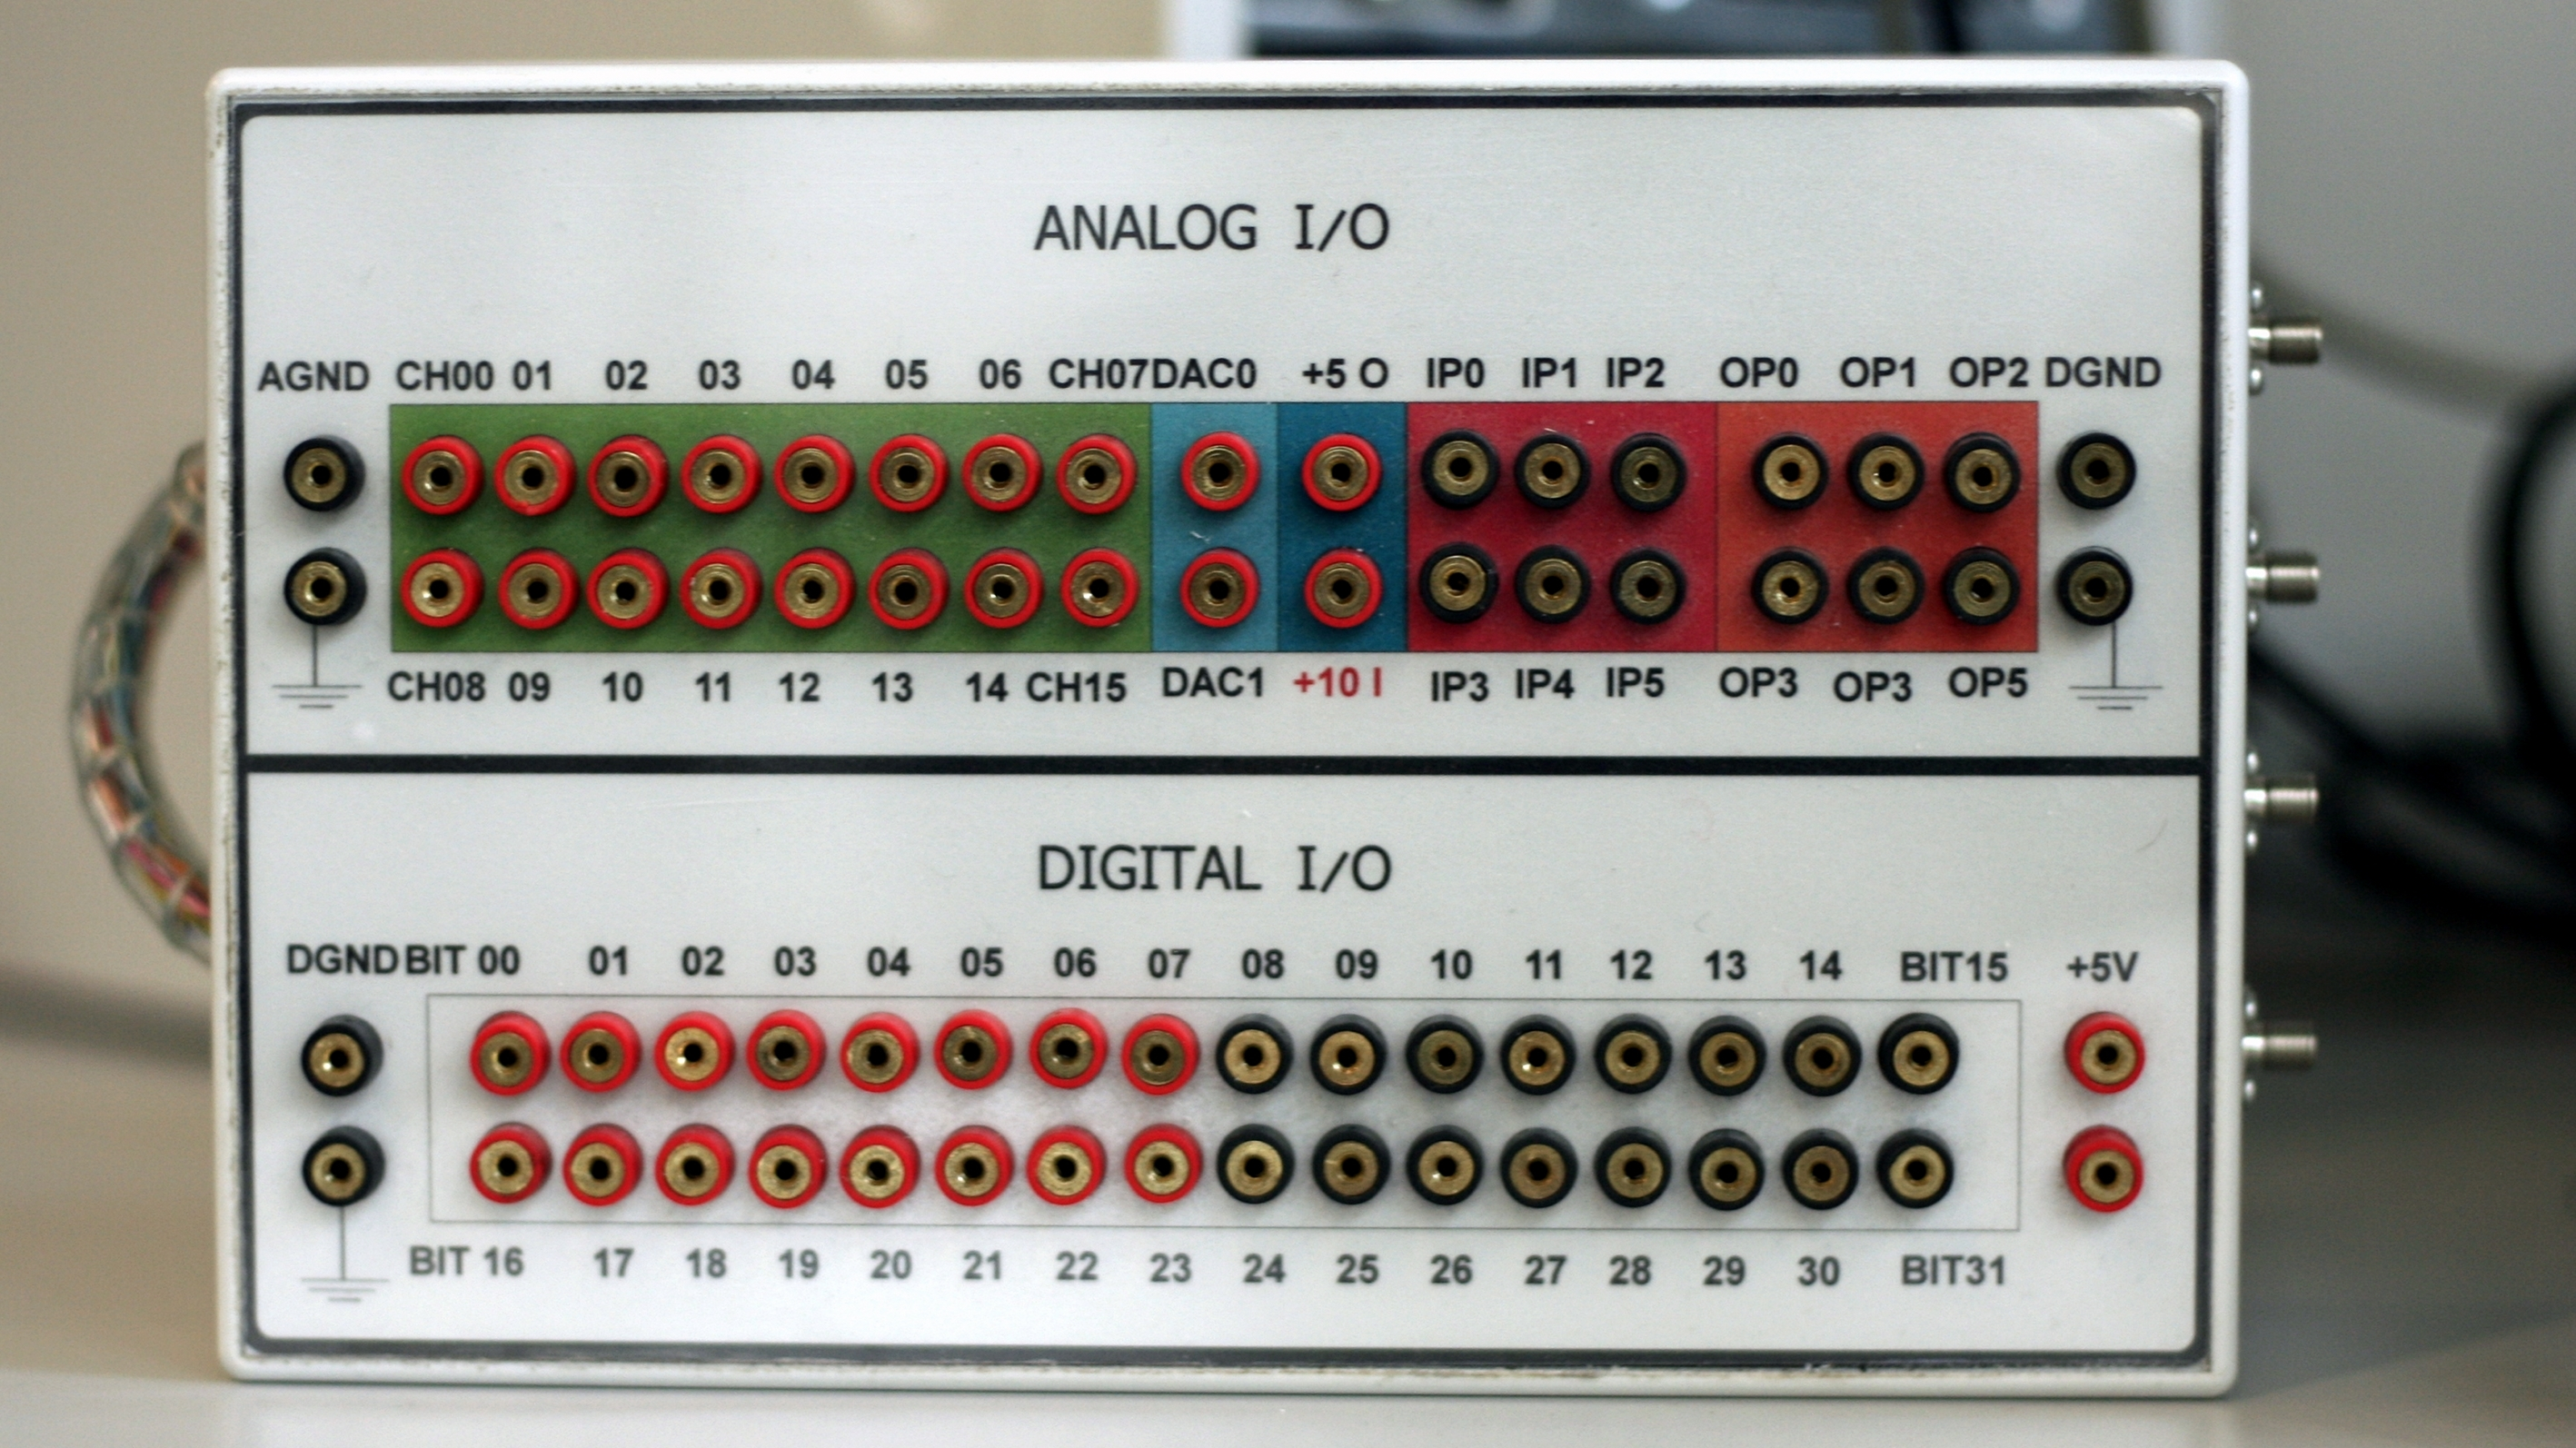
\includegraphics[scale=1, keepaspectratio=true]
		{gis-pfc-ch2-05.jpg}
	\end{center}
	\caption[Plano de la caja de conexiones ya terminada] {Plano de la
	caja de conexiones ya terminada.}
	\label{fig:conbox}
\end{figure}


\part{Ensayos no destructivos con ultrasonidos}

\chapter{Dise�o del dispositivo de ultrasonidos}


\section{Introducci�n te�rica a las inspecciones mediante ultrasonidos}


\subsection{Fundamentos de ultrasonidos}

Los ultrasonidos son ondas ac�sticas de naturaleza mec�nica o el�stica como los sonidos. A diferencia de las ondas s�nicas los ultrasonidos se encuentran en una banda de frecuencia superior. Dicha banda parte de los 20 kHz y, carente de un l�mite f�sico, llega hoy hasta los 1000 MHz debido a limitaciones tecnol�gicas. Las frecuencias empleadas en los ensayos no destructivos se encuentran entre los 20 kHz y los 25 MHz. Cabe remarcar que las propiedades de las ondas ac�sticas se mantienen invariantes con la frecuencia, y por tanto, son comunes dentro del espectro ac�stico.\par
Las ondas ultras�nicas son perturbaciones mec�nicas que viajan a trav�s de un medio el�stico, por tanto, la condici�n primordial para que las ondas ultras�nicas se propaguen a trav�s de un medio es que este contenga fracciones de materia tales como �tomos o mol�culas susceptibles de vibrar. El medio determina tambi�n que modos de propagaci�n pueden adoptar las ondas ultras�nicas que se propagan a su trav�s. Frecuentemente se asocia un nombre caracter�stico a las ondas ultras�nicas en funci�n del modo en el que se propagan por el medio. A continuaci�n se exponen los modos de propagaci�n de mayor relevancia.

\begin{itemize}
	\item Las \emph{ondas longitudinales}, tambi�n llamadas \emph{ondas de presi�n o compresi�n}, son aquellas que oscilan en la direcci�n de propagaci�n. Al contrario que el resto de modos de propagaci�n que s�lo se dan en s�lidos, el modo longitudinal puede estar presente tambi�n en l�quidos y gases.
	\item En las \emph{ondas transversales o de cizalladura} las oscilaciones se producen en la direcci�n perpendicular a la direcci�n de propagaci�n.
	\item Las \emph{ondas de superficie} se propagan �nicamente a trav�s de s�lidos semi"=infinitos cuya superficie sea plana o curva y siempre siguiendo las irregularidades del contorno del mismo.
	\item Las \emph{ondas de Lamb o de chapa} son propias de medios s�lidos en los que el espesor es del mismo orden que la longitud de onda, provocan la vibraci�n de todo el material.
\end{itemize}

La energ�a ac�stica que se propaga por un medio se manifiesta en forma de presi�n ac�stica, esta a su vez define el campo ac�stico. La presi�n ac�stica se define como:

\begin{equation}
	p = Z\cdot v
	\label{eq:acuospressure}
\end{equation}

Ecuaci�n en la que $v$ representa la velocidad de vibraci�n y $Z$ la impedancia ac�stica. La impedancia ac�stica es una medida de con que resistencia se oponen los elementos de masa de un medio a la vibraci�n provocada por las ondas ac�sticas, en ning�n caso da una relaci�n de la resistencia con la que el medio se opone a la propagaci�n de la onda ac�stica. Es una constante del medio que aumenta con la cohesi�n de sus mol�culas, y puede expresarse en funci�n de la densidad $\rho_0$ y de la velocidad de propagaci�n de las ondas ultras�nicas en dicho medio $c$.

\begin{equation}
	Z = \rho_0\cdot c
	\label{eq:Zacoustic}
\end{equation}


\subsection{Campo ac�stico generado por un transductor}\label{subsec:field}

La excitaci�n el�ctrica de un transductor produce una onda de presi�n que se propaga en el medio siguiendo las leyes f�sicas de la propagaci�n de ondas y, en particular, los principios de superposici�n de Huygens\footnote{El tratamiento que se da en esta secci�n a los transductores de ultrasonidos es similar al que la teor�a de antenas da a las antenas de apertura conocidas como bocinas. Para un mayor detalle consultar el texto de Stutzman y Thiele, \cite{stutzman1997atd}.}. Se denomina campo ac�stico a la distribuci�n temporal y espacial de la presi�n ac�stica a la que se someten las part�culas materiales del medio en el que se propagan las ondas ac�sticas. Las caracter�sticas del campo ac�stico dependen principalmente de aspectos geom�tricos del transductor.\par
La regi�n del campo ac�stico m�s pr�xima al transductor se conoce como campo pr�ximo o cercano. Tambi�n recibe el nombre de campo de interferencia debido a que en esa regi�n el campo est� constituido por m�ximos y m�nimos que surgen como resultado de las interferencias que se producen entre las se�ales originadas en los distintos puntos del transductor. El m�ximo principal del campo ac�stico delimita la regi�n de campo pr�ximo. La longitud de esta regi�n puede calcularse a partir del di�metro del transductor $D$, o en su defecto a partir de la dimensi�n principal de este.

\begin{equation}
	L_0 = \frac{D^2}{4\lambda}
	\label{eq:nearfield}
\end{equation}

M�s all� del campo cercano encontramos el campo lejano. En el campo lejano el frente de ondas de la radiaci�n ac�stica empieza a divergir. Se llama �ngulo de divergencia del haz a la raz�n con la que el haz se expande y se emplea el s�mbolo $\gamma_0$ para representarla. Puede calcularse $\gamma_0$ a partir de la siguiente expresi�n.

\begin{equation}
	\sin{\gamma_0} = 1.2\cdot\frac{\lambda}{D}
	\label{eq:Adivergence}
\end{equation}

\begin{figure}
	\begin{center}
		
\includegraphics{gis-pfc-ch3-1.mps}
	\end{center}
	\caption{Diagrama simplificado que muestra el campo ac�stico generado por un transductor cil�ndrico}
	\label{fig:transceiver}
\end{figure}

En la \vref{fig:transceiver} el lector puede observar una representaci�n del campo ac�stico generado por un transductor de ultrasonidos cil�ndrico. Puede observarse la forma geom�trica del campo pr�ximo tal y como se ha considerado en este documento: un cilindro de radio igual al del transductor y altura $L_0$. En el interior del cilindro el campo ac�stico permanece constante y en el exterior el campo es nulo. A continuaci�n se ilustra como el frente de ondas diverge en el campo lejano. La figura empleada para representar el campo lejano es un tronco de cono en cuyo interior el campo ac�stico ir�a incrementando de la superficie al eje.\par
Para finalizar este punto cabe mencionarse que el transductor es responsable de que una determinada regi�n de los materiales inspeccionados no pueda ser caracterizada mediante el uso de ultrasonidos. La raz�n es que tras emitir un pulso ac�stico un transductor no cesa inmediatamente de vibrar, si no que lo sigue haciendo durante cierto tiempo a su frecuencia natural de oscilaci�n con un factor de amortiguamiento que depende de factores constructivos. A la regi�n del material que no puede ser inspeccionada se la conoce como zona muerta o zona ciega. La zona ciega de un material empieza en la superficie que est� en contacto con el transductor y su profundidad depende de la duraci�n de los pulsos ac�sticos.


\subsection{T�cnicas empleadas en las inspecciones ultras�nicas}\label{subsec:technics}

Atendiendo a la situaci�n del receptor en los ensayos no destructivos mediante ultrasonidos se distinguen dos t�cnicas: la t�cnica de pulso"=eco y la t�cnica de transmisi�n. En la t�cnica de pulso"=eco el receptor suele encontrarse cercano al emisor, de hecho es frecuente que un mismo transductor haga las veces de emisor y receptor. Por el contrario en la t�cnica de transmisi�n el receptor se coloca alineado en el eje del emisor pero en el extremo opuesto del material inspeccionado.\par

\begin{figure}
	\begin{center}
		\subfloat[Inspecci�n ultras�nica por transmisi�n]{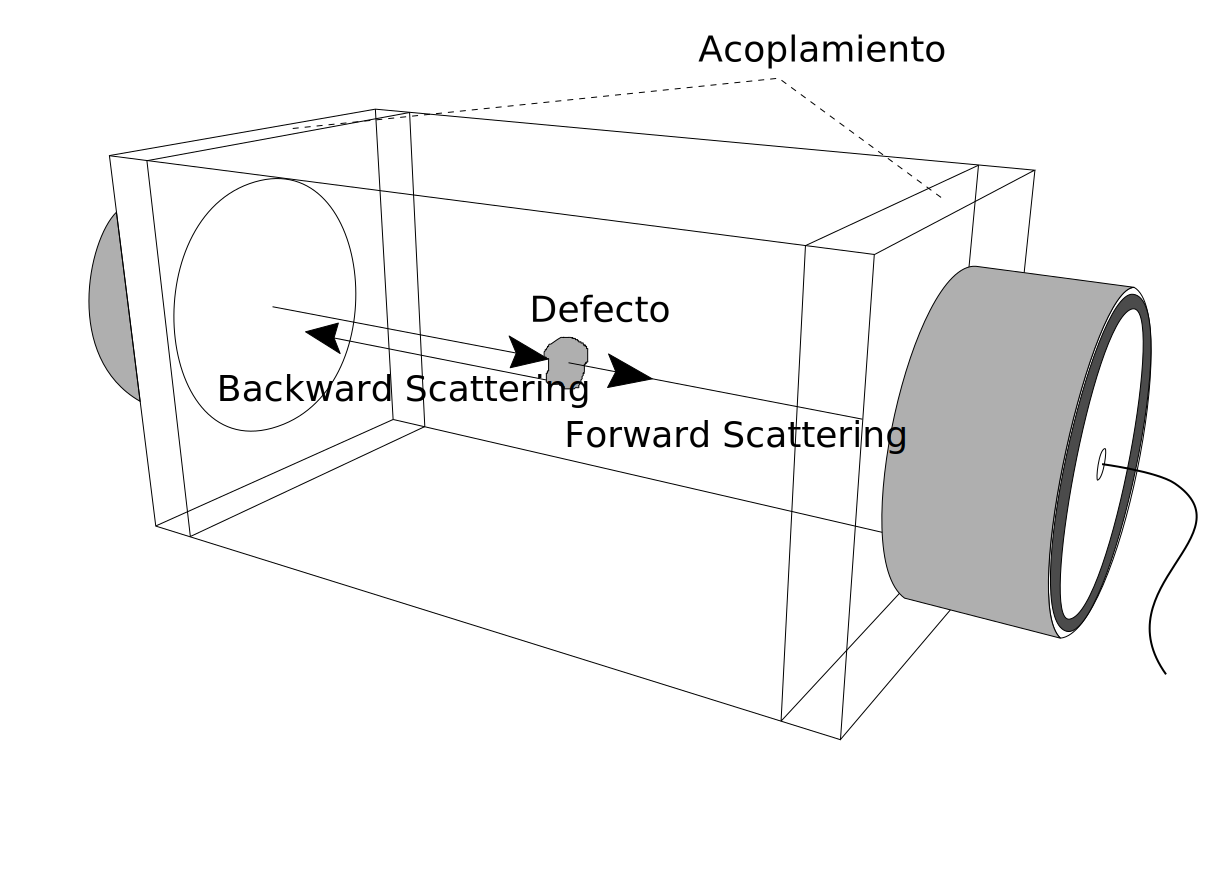
\includegraphics{gis-pfc-ch3-2.mps}}\bigskip\par
		\subfloat[Inspecci�n ultras�nica por pulso"=eco]{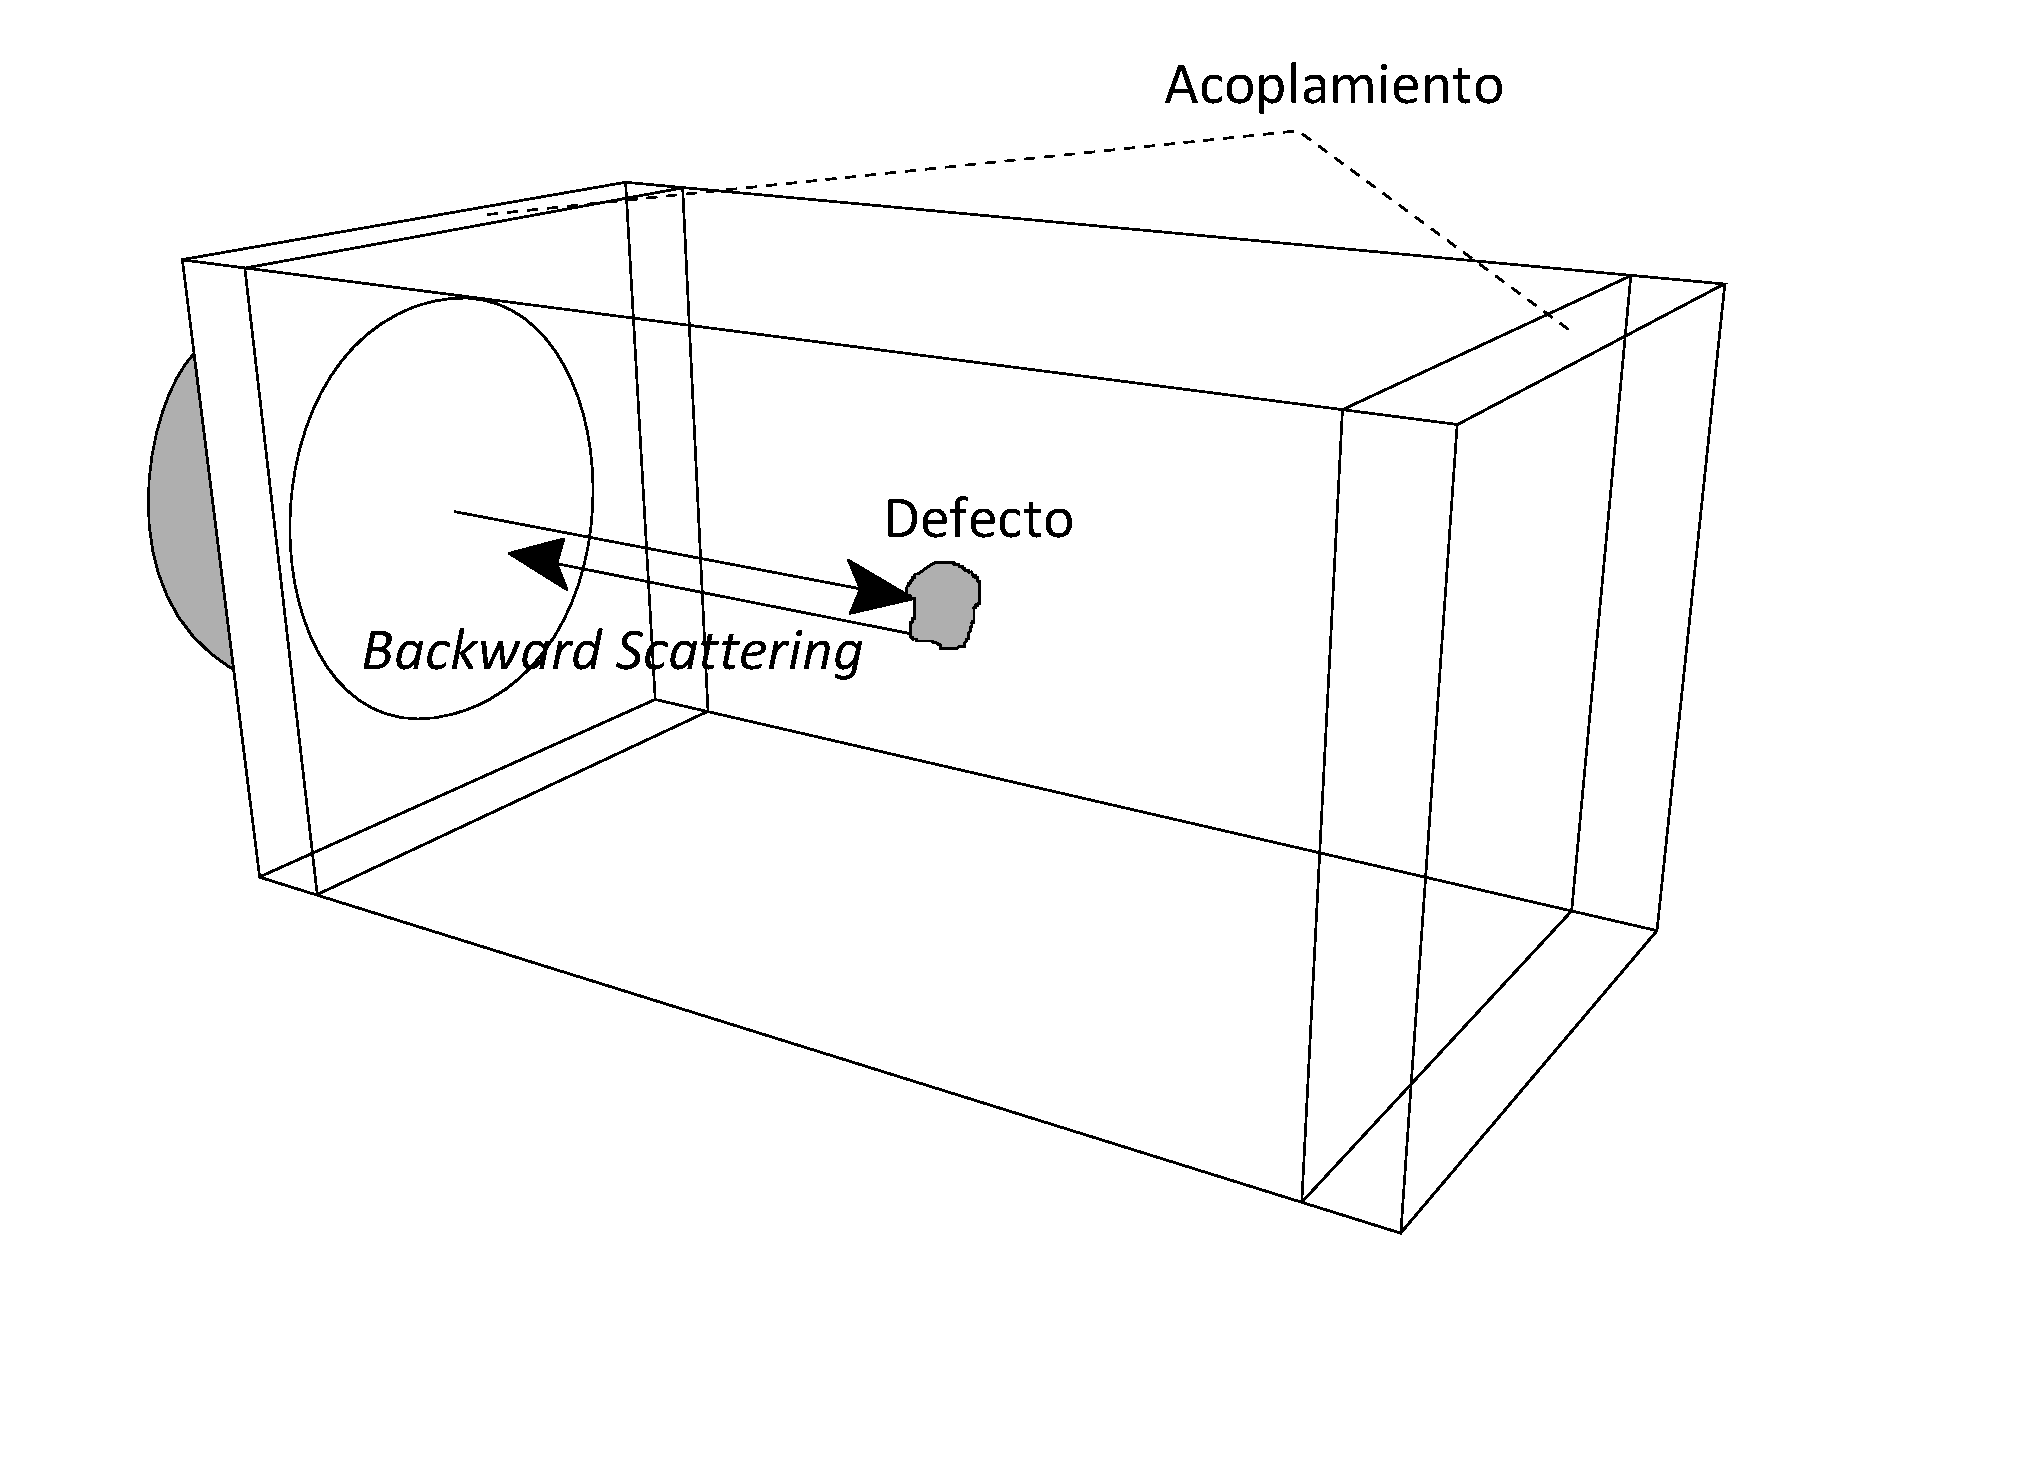
\includegraphics{gis-pfc-ch3-3.mps}}
	\end{center}
	\caption{Diferencias en cuanto al n�mero y posici�n de los transductores seg�n la t�cnica empleada en una evaluaci�n mediante ultrasonidos}
	\label{fig:technics}
\end{figure}

Al propagarse un pulso ac�stico por el medio, parte de �ste se refleja al encontrarse con discontinuidades en la impedancia ac�stica, otra parte seguir� avanzando hasta atravesar el material o verse completamente atenuada. La se�al que capta el receptor depende de su ubicaci�n. De este modo la se�al recibida cuando la t�cnica empleada es la de pulso"=eco es la suma de los pulsos reflejados o ecos. Si la t�cnica utilizada es la t�cnica de transmisi�n se percibe el pulso original, modificado por haber atravesado el medio. La informaci�n que contiene la se�al recibida es, por tanto, diferente.\par
La t�cnica de pulso"=eco se centra en el estudio de la amplitud, forma y posici�n temporal de los ecos. La t�cnica de transmisi�n por su parte observa posibles cambios de velocidad en el pulso ac�stico y mide la atenuaci�n que �ste experimenta al pasar a trav�s del medio. La informaci�n que proporciona el estudio de los ecos es m�s rica pero tambi�n m�s compleja. Por consiguiente la elecci�n de una u otra t�cnica est� supeditada no s�lo a las posibilidades de inspecci�n que ofrece el medio, si no tambi�n al tipo de informaci�n que se pretende obtener con el ensayo.


\subsection{Par�metros de calidad en una inspecci�n}\label{subsec:quality}

Los par�metros de calidad proporcionan una medida cualitativa de la bondad de un ensayo. Los m�s empleados son resoluci�n, linealidad y relaci�n se�al a ruido.\par
En ensayos no destructivos la resoluci�n es la distancia m�nima (o una medida en relaci�n con �sta) a la que deben encontrarse dos singularidades cercanas para que ambas sean detectadas distingui�ndose una de la otra. Se hace distinci�n entre resoluci�n axial y resoluci�n lateral. La primera alude a la distancia que debe haber entre dos singularidades alineadas en la direcci�n longitudinal de propagaci�n de las ondas ac�sticas, la segunda a la que debe haber entre singularidades que se encuentren dispuestas en una l�nea normal a esa direcci�n.\par
Atendiendo a la definici�n de resoluci�n que se ha proporcionado, se considera que la resoluci�n es mejor si la distancia m�nima disminuye y peor si �sta aumenta. Teniendo esto en cuenta, para mejorar la resoluci�n axial de un sistema es necesario emplear dispositivos de banda ancha y emitir pulsos estrechos de alta frecuencia. La frecuencia de los pulsos ac�sticos est� limitada por el espesor del medio, a medida que aumenta la frecuencia disminuye la profundidad de penetraci�n del pulso, resulta pues conveniente adoptar una soluci�n de compromiso.\par
La resoluci�n lateral depende tambi�n de la frecuencia del pulso, es mejor a medida que aumenta la frecuencia puesto que disminuye la longitud de onda. Adem�s depende del di�metro de los transductores, es peor cuanto m�s anchos son �stos. Y en la regi�n de campo lejano, la resoluci�n lateral empeora a medida que aumenta la profundidad.\par
El comportamiento de la resoluci�n lateral con respecto al di�metro del transductor y la frecuencia del pulso ac�stico transmitido, descrito en el p�rrafo anterior puede deducirse de las ecuaciones \eqref{eq:nearfield} y \eqref{eq:Adivergence}. Puede observarse que, a medida que aumenta la frecuencia y disminuye la longitud de onda del pulso, aumenta la longitud de la regi�n de campo cercano. En dicha regi�n el campo ac�stico se encuentra contenido en un cilindro de radio el del transductor, como ya se ha mencionado, y a partir de ah� empieza a divergir seg�n una raz�n que disminuye con la longitud de onda. Para una mejor resoluci�n es pertinente que la regi�n activa del campo ultras�nico sea lo m�s estrecha posible, de ese modo se evita en la medida de lo posible que dos anomal�as cercanas queden cubiertas por el haz en un mismo evento de la secuencia de barrido. Por tanto, se confirma por medio de estas ecuaciones los beneficios en t�rminos de resoluci�n que redundan del uso de transductores de di�metro estrecho y de pulsos ultras�nicos de alta frecuencia.\par
La definici�n y comportamiento de linealidad y relaci�n se�al a ruido son los habituales en t�rminos de sistemas electr�nicos, por eso se entiende que el lector tiene una noci�n al respecto y no se dan m�s aclaraciones en este apartado.


\subsection{El problema del ruido en las inspecciones}

La principal limitaci�n en las inspecciones ultras�nicas es el ruido. Los ensayos de este tipo se ven afectados generalmente por varias fuentes de ruido. Seg�n su naturaleza estad�stica el ruido perjudica en mayor o menor medida los resultados de un ensayo. Cuanto m�s se asemeje el ruido a la se�al desde el punto de vista estad�stico m�s la perjudicar� y m�s dif�cil ser� contrarrestar su efecto. El \emph{ruido incoherente aleatorio} tiene, como su propio nombre indica, un origen aleatorio, y en consecuencia no est� relacionado con la se�al. Por el contrario, los mecanismos que originan el \emph{ruido coherente} son con frecuencia los mismos que dan lugar a la se�al de inter�s, y de ah� que exista una fuerte relaci�n entre el car�cter estad�stico de ambas se�ales.\par
Entre los exponentes m�s comunes de ruido incoherente aleatorio encontramos el \emph{ruido gaussiano} y el \emph{ruido impulsivo}. El primero es inherente a los equipos electr�nicos y su origen es t�rmico, el segundo tiene origen en las interferencias electromagn�ticas causadas por equipos el�ctricos situados en las proximidades del sistema empleado para el ensayo. Este tipo de ruido puede ser combatido sin dificultad con t�cnicas bien conocidas como son: el promediado temporal de se�ales, el filtrado paso-banda, la autocorrelaci�n o las t�cnicas de compresi�n de pulsos, en el caso del ruido gaussiano; y algoritmos de filtrado no lineal, en el caso del ruido impulsivo.\par
En ensayos no destructivos mediante ultrasonidos, la se�al de inter�s y el \emph{ruido estructural o de grano} tienen una misma procedencia. Ambas se�ales surgen como consecuencia de interactuar un pulso ac�stico con los distintos elementos de que se compone un material. En el caso de la primera de las se�ales, el pulso se refleja en las posibles particularidades presentes en el medio como grietas o hendiduras. En el caso del ruido, las reflexiones se producen al encontrarse el pulso con las part�culas suspendidas en el medio y de que �ste se compone. Las diferencias entre ambas se�ales radican en el tama�o y distribuci�n de los elementos reflectantes en el medio. Los reflectores que provocan el ruido son de tama�o inferior a la longitud de onda de la se�al propagada, y se encuentran cercanos entre s� dispuestos de forma aleatoria por el medio. Esto provoca que el car�cter de la se�al que aqu� se ha bautizado como ruido estructural sea, a efectos de una inspecci�n ultras�nica, aleatorio e impredecible. Si bien, la naturaleza de estas se�ales es similar y en concreto lo es su naturaleza estad�stica. Por eso el ruido estructural es considerado un ruido de tipo coherente y resulta complicado neutralizar su efecto en los resultados del ensayo. A�n m�s, este ruido es el principal factor limitante en ensayos de este tipo, enmascarando detalles en la se�al de inter�s que aportan informaci�n sobre posici�n, tama�o y forma de las singularidades que son objeto de estudio. En contraposici�n a este hecho, es posible emplear esta se�al, que aqu� es indeseada y considerada ruido, en otro tipo de trabajos con el objetivo de caracterizar las propiedades ac�sticas de un material.


\subsection{Fundamentos f�sicos del ruido estructural}

El ruido estructural es una consecuencia directa de la dispersi�n. Cuando un frente de ondas incide sobre una part�cula de tama�o comparable a su longitud de onda, la energ�a que transporta se dispersa por la acci�n de esa part�cula. Dicha part�cula act�a como un reflector esf�rico y selectivo en frecuencia ---afectando m�s a las altas frecuencias\footnote{Seg�n la relaci�n $c = \lambda\cdot f$, si se mantiene $c$, a medida que aumenta $f$ disminuir� la longitud de onda y, por tanto, el tama�o de la part�cula con respecto a la longitud de onda aumentar�.}--- que refleja la se�al en todas direcciones. De este modo, aquellos materiales que contienen un n�mero considerable de part�culas susceptibles de interferir del modo descrito en la propagaci�n de un determinado frente de ondas, son considerados materiales dispersivos.\par
En el caso de un frente de ondas ac�sticas que incide sobre un determinado material dispersivo, la energ�a que tras el proceso de reflexi�n se propaga en sentido contrario al sentido de propagaci�n del frente de ondas se conoce como \emph{back-scattering}. Por su parte, la energ�a perturbada por la acci�n del reflector que contin�a propag�ndose en el mismo sentido suele denominarse \emph{forward-scattering}. En los \sig{endus} dependiendo de la t�cnica empleada es uno u otro tipo de dispersi�n el que causa un mayor deterioro de los resultados: si la t�cnica empleada es de pulso"=eco, el \emph{back-scattering} ser� el m�s perjudicial; si, por el contrario, se est� empleando la t�cnica de transmisi�n, ser� el \emph{forward-scattering} el m�s nocivo para el proceso.\par
Para poder estudiar el efecto del ruido estructural en las inspecciones ultras�nicas de forma adecuada es necesario caracterizar el proceso de emisi�n"=recepci�n que se da en un ensayo mediante ultrasonidos desde el punto de vista de la respuesta al impulso o r�gimen transitorio.


\subsubsection{An�lisis del proceso de emisi�n-recepci�n}

Los diferentes elementos que intervienen en el proceso de emisi�n"=recepci�n de que consta una inspecci�n ultras�nica tienen un comportamiento lineal, esto permite estudiar todo el conjunto como un sistema lineal, y ello a su vez posibilita el uso de t�cnicas propias del an�lisis de este tipo de sistemas.\par
Sup�ngase un transductor de perfil arbitrario, al excitarse con un pulso el�ctrico, $u(t)$, y dadas a sus propiedades electromec�nicas, emite un pulso ac�stico de velocidad $v(t)$ relacionado con la respuesta impulsiva de emisi�n del transductor, $h_{te}(t)$.

\begin{equation}
	v(t) = h_{te}(t)\otimes u(t)
	\label{eq:emiter}
\end{equation}

La respuesta impulsiva electrodin�mica en emisi�n, $h_{te}(t)$ depende del circuito electr�nico empleado para excitar el transductor y de los par�metros de dise�o de este �ltimo.\par
La presi�n en un punto situado en el eje $y$ y a una distancia $z$ del transductor es el resultado de la suma coherente de las aportaciones de cada uno de los puntos que forman la cara del transductor por la que emite la onda ac�stica, consider�ndolos como emisores omnidireccionales y esf�ricos. La presi�n en cada punto del espacio est� relacionada con la velocidad en la cara del pist�n por medio de la siguiente expresi�n:

\begin{equation}
	p(z, t) = \rho\,\frac{\partial}{\partial t}\left\{v(t)\otimes h_{m}(z, t)\right\}
	\label{eq:diffracpressure}
\end{equation}

Siendo $\rho$ la densidad del medio por la que se propaga la onda ac�stica y $h_{m}(z, t)$ la respuesta al impulso en el medio de propagaci�n considerando la difracci�n que se produce en dicho medio.\par
La propagaci�n de una onda ac�stica se ve sometida a fen�menos de difracci�n propios de la naturaleza ondulatoria de la radiaci�n ac�stica y fen�menos de atenuaci�n a consecuencia de la interacci�n con el medio. De cara al estudio de la propagaci�n de la onda estos fen�menos pueden tratarse por separado. Por un lado se considera el efecto de la difracci�n sobre la onda en un medio homog�neo y sin p�rdidas, y por otro la atenuaci�n que induce el medio. Esta aproximaci�n mantiene su validez siempre que el estudio afecte a una regi�n del campo muy pr�xima al transductor. Si se considera esta aproximaci�n, y se tiene $h_d(z, t)$, la respuesta al impulso en un medio homog�neo y sin p�rdidas a la difracci�n, y $a(z, t)$, la atenuaci�n atribuida al medio; puede descomponerse la respuesta al impulso en el medio de propagaci�n a la difracci�n en esos dos t�rminos:

\begin{equation}
	h_m(z, t) = h_d(z, t)\otimes a(z, t)
	\label{eq:diffraction}
\end{equation}

La atenuaci�n es selectiva en frecuencia y ello se asocia a los siguientes aspectos derivados de la existencia de una macro y una micro"=estructura en el material:

\begin{itemize}
	\item La absorci�n o transformaci�n de la energ�a ac�stica que transporta la onda en calor.
	\item Y los efectos de dispersi�n de la energ�a.
\end{itemize}

La expresi�n que define la atenuaci�n sufrida por la onda ac�stica toma la siguiente forma a partir de $\alpha(\omega)$ o coeficiente de atenuaci�n caracter�stico del medio.

\begin{equation}
	A(z, \omega) = e^{\int^z_0 -\alpha(z, \omega)dz} 
	\label{eq:loss}
\end{equation}

Cuando la onda ac�stica incide sobre un reflector, las caracter�sticas de �ste determinan la relaci�n entre la onda incidente y la reflejada. Esta relaci�n viene dada por la funci�n de reflectividad, $h_r(t)$, que depende de la frecuencia de la onda de presi�n. Si la reflexi�n que se produce al llegar la onda hasta la part�cula es especular, $h_r(t)$ coincide con una delta de Dirac ponderada.\par
Como consecuencia de la reflexi�n, una se�al distinta de la emitida por el transductor en origen regresa a �ste. Por tanto, se produce en la cara del transductor que da al material una presi�n variable con el tiempo $p_R(z, t)$, constituida por la suma de la presi�n que se produce en cada punto de la mencionada superficie.\par

\begin{equation}
	p_R(z, t) = p(z, t)\otimes h_r(t)\otimes h_m(z, t)
	\label{eq:recpressure}
\end{equation}

Del mismo modo, parte de la se�al reflejada avanza en el mismo sentido de propagaci�n que la onda incidente. Si no es dispersada completamente en el medio avanza hasta atravesar el material por completo. En ese caso, si es la t�cnica de transmisi�n la t�cnica empleada, una presi�n semejante a $p_R(z, t)$ se produce en la cara del transductor que se encuentra al otro extremo del material. La funci�n de reflectividad no var�a, tan s�lo cambia la distancia que debe atravesar el frente de ondas hasta alcanzar el transductor y, por tanto, es diferente la contribuci�n de la respuesta al impulso en el medio a la difracci�n, $h_m(z^\prime, t)$ en el segundo trayecto.\par
Finalmente, la presi�n $p_R$ se traduce en una se�al el�ctrica en bornes del transductor. Esta se�al est� relacionada con la respuesta impulsiva del transductor en recepci�n, $h_{tr}(t)$, que depende, al igual que $h_{te}(t)$ del circuito acondicionador y del proceso de fabricaci�n del transductor.

\begin{equation}
	y(t) = h_{tr}(t)\otimes p_R(z, t)
	\label{eq:receiver}
\end{equation}

Por consiguiente el proceso de emisi�n"=recepci�n en el que se fundamentan los \sig{endus} puede describirse mediante la respuesta impulsional en cascada de todos los fen�menos descritos.

\begin{equation}
	y(t) = \rho_0\frac{\partial}{\partial t}\left\{u(t)\otimes h_{te}(t)\otimes h_d(z, t)\otimes a(z, t)\otimes h_r(t)\otimes h_d(z, t)\otimes a(z, t)\otimes h_{tr}(t)\right\}
	\label{eq:emirec}
\end{equation}

La figura \vref{fig:emirecmodel} muestra un diagrama de bloques que representa el proceso de emisi�n"=recepci�n y todos los fen�menos que en el intervienen seg�n el modelo empleado en este documento. La funci�n de transferencia del sistema puede obtenerse de modo sencillo aplicando el teorema de la convoluci�n.

\begin{figure}
	\begin{center}
		\includegraphics[scale=1, keepaspectratio=true]{gis-pfc-ch3-4.mps}
	\end{center}
	\caption{Diagrama de bloques que representa el proceso de emisi�n"=recepci�n y todos los elementos que en el intervienen (considerando el modelo propuesto)}
	\label{fig:emirecmodel}
\end{figure}

\begin{equation}
	Y(\omega) = j\omega\rho_0\cdot U(\omega)\cdot H_{te}(\omega)\cdot H^2_d(z, \omega)\cdot A^2(z, \omega)\cdot H_r(\omega)\cdot H_{tr}(\omega)
	\label{eq:transference}
\end{equation}

Aprovechando la linealidad del sistema se agrupan los t�rminos de la funci�n de transferencia en \vref{eq:groupedtransference}, para que el resultado quede en funci�n de la respuesta electromec�nica del transductor, $X(\omega)$, y de la respuesta espacial al impulso, $H(z, \omega)$.

\begin{equation}
	Y(\omega) = X(\omega)\cdot H(z, \omega)\cdot A^2(z, \omega)
	\label{eq:groupedtransference}
\end{equation}

\begin{equation}
	X(\omega) = j\omega\rho_0\cdot U(\omega)\cdot H_{te}(\omega)\cdot H_{tr}(\omega)
	\label{eq:transducer}
\end{equation}

Siendo esta �ltima, la respuesta espacial al impulso, funci�n de la posici�n del reflector y de su forma, o lo que es lo mismo, de las funciones de reflectividad y difracci�n.

\begin{equation}
	H(z, \omega) = H^2_d(z, \omega)\cdot H_r(\omega)
	\label{eq:spacialresponse}
\end{equation}

Al agrupar de este modo la funci�n de transferencia se establece de forma expl�cita la separaci�n entre los procesos de difracci�n y atenuaci�n. Adem�s es posible establecer nuevas separaciones: dejando por un lado los efectos debidos a los transductores y electr�nica de acondicionamiento, $X(\omega)$; por otro la influencia del medio en la onda que se propaga, es decir, la atenuaci�n, $A(z, \omega)$; y, finalmente, por otro los efectos de la propagaci�n y la interacci�n con el reflector, $H(z, \omega)$.


\subsubsection{Atenuaci�n en medios dispersivos}

La atenuaci�n es el fen�meno en el que se manifiesta la influencia del medio en la propagaci�n de una onda. Suponiendo un medio en el que la atenuaci�n depende �nicamente de la frecuencia de la onda ac�stica, puede calcularse la atenuaci�n sufrida por dicha onda tras haberse propagado una distancia $z$ a lo largo del medio, como:

\begin{equation}
	A(z, \omega) = e^{-\alpha(\omega)\cdot z}
	\label{eq:independentloss}
\end{equation}

Donde, como se anticip� en \vref{eq:loss}, $\alpha(\omega)$ es el coeficiente de atenuaci�n.\par
Cuando el material por el que se propaga la onda es no homog�neo, la atenuaci�n se debe a dos fen�menos:

\begin{description}
	\item[Absorci�n.] Fen�meno que tambi�n aparece en medios homog�neos y por el cual la energ�a que transporta la onda se transforma en otro tipo de energ�a, por lo general en calor.
	\item[Dispersi�n.] En este estudio se entiende dispersi�n como la distorsi�n que ejerce sobre el frente de ondas el grano suspendido en el medio. La acci�n del borde del grano, as� como los saltos de �ndice de refracci�n que provoca la presencia de ese grano en el medio, contribuyen a la aparici�n de este fen�meno.
\end{description}

En el coeficiente de atenuaci�n global vienen reflejadas las acciones que sobre la se�al ejercen ambos fen�menos. Siendo $\alpha_s(\omega)$ la contribuci�n de la dispersi�n y $\alpha_a(\omega)$ la contribuci�n de la absorci�n.

\begin{equation}
	\alpha(\omega) = \alpha_a(\omega) + \alpha_s(\omega)
	\label{eq:losscoefficient}
\end{equation}

El coeficiente de absorci�n depende del cuadrado de la frecuencia a la que oscila el frente de ondas, $\alpha_a(\omega) = a_1\omega^2$. Siendo $a_1$ la constante de absorci�n del material. Por su parte, $\alpha_s(\omega)$ depende del tama�o, forma, orientaci�n y distribuci�n de los granos en el medio, aunque tambi�n de la frecuencia como se muestra a continuaci�n.


\subsubsection{Estimaci�n del coeficiente de dispersi�n para un material dispersivo de naturaleza granulosa}

El coeficiente de dispersi�n de un material no homog�neo de naturaleza granulosa puede estimarse de forma te�rica asumiendo que los granos en el medio forman una matriz tridimensional de peque�os reflectores o granos esf�ricos, tal y como se muestra en la figura \vref{fig:matrix}. Asumiendo este modelo, puede obtenerse la respuesta global del medio obteniendo la respuesta de un reflector e integrando a todo el volumen el resultado obtenido para un solo grano.

\begin{figure}
	\begin{center}
		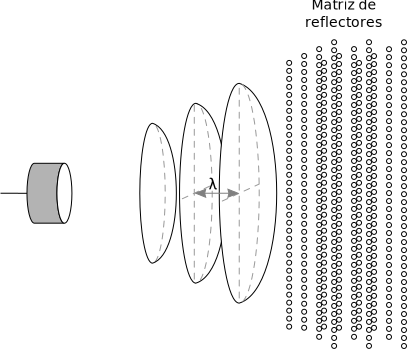
\includegraphics[scale=1, keepaspectratio=true]{gis-pfc-ch3-5.mps}
	\end{center}
	\caption{Modelo de peque�os receptores para estimaci�n del coeficiente de dispersi�n}
	\label{fig:matrix}
\end{figure}

La \vref{eq:disperser} es una aproximaci�n de la respuesta espacial al impulso de un solo dispersor cuando sobre el incide un frente de ondas ultras�nicas longitudinales plano. En esta ecuaci�n se han empleado: $k$, constante que depende de la geometr�a del reflector; la frecuencia angular a la que oscila el frente de ondas, $\omega$; $c_l$, o velocidad a la que se propaga el frente de ondas; $V$ volumen del dispersor; y $z$ distancia entre �ste y el transductor.

\begin{equation}
	H_s(z, \omega) = k\,\frac{V\omega^2}{zc^2_l}\,e^{-j2\omega z/c}
	\label{eq:disperser}
\end{equation}

De $H_s(z, \omega)$ se deduce que la onda reflejada es dependiente de la frecuencia angular de oscilaci�n. De hecho, se manifiestan las propiedades de filtro paso bajo que muestra la part�cula. Si el reflector es de tama�o muy superior a la longitud de onda de la radiaci�n ac�stica, la dependencia de $H_s(z, \omega)$ con $\omega$ es en la pr�ctica despreciable, y s�lo depender�a de la geometr�a del reflector.\par
Si el conjunto de dispersores suspendidos en el medio es homog�neo, y todos ellos est�n equiespaciados y presentan isotrop�a, es posible suponer que el frente de ondas se encuentra de forma sucesiva y peri�dica con planos de reflectores. Si se supone adem�s que la contribuci�n de la dispersi�n m�ltiple es despreciable frente a la contribuci�n de las reflexiones primarias, el frente de ondas que se propaga tras el primer plano de part�culas es la suma vectorial de la onda no dispersada y de una peque�a fracci�n de la onda que tras interactuar con dichas part�culas sigue propag�ndose en la misma direcci�n en la que se propaga el frente de ondas. Si se tiene en cuenta el comportamiento de un plano de reflectores, semejante a un filtro paso bajo, el resultado de la dispersi�n es \emph{un frente de ondas que con respecto al original tiene atenuadas las altas frecuencias}. Por tanto, puede manifestarse un equivalente, \emph{un material dispersivo se comporta como un filtro paso bajo cuya caracter�stica de atenuaci�n depende de la profundidad que haya alcanzado la onda en su propagaci�n}.\par
Puede escribirse una expresi�n de la atenuaci�n causada por la dispersi�n si se considera �sta en funci�n de la energ�a neta que aporta al frente de ondas cada uno de los planos reflectores. Esta expresi�n queda en funci�n del di�metro del grano $D$, y de $s_1$, una constante de dispersi�n que depende del material.

\begin{equation}
	A_s(z, \omega) = e^{-s_1D^3\omega^4z}
	\label{eq:dispersionloss}
\end{equation}

Mediante esta expresi�n y la \vref{eq:independentloss}, aplicando la \vref{eq:losscoefficient}, es posible calcular el coeficiente de atenuaci�n debido a la dispersi�n, $\alpha_s$, en la regi�n de Rayleigh, en la que $D\ll\lambda$. Empleando deducciones semejantes puede obtenerse el coeficiente de atenuaci�n en distintas situaciones de tama�o de grano y longitud de onda.

{\setlength{\extrarowheight}{0.5ex}
\begin{equation}
	\alpha_s(\omega) = \left\{
	\begin{array}{c@{\qquad\text{---}\qquad}c@{\quad}c}
		s_1D^3\omega^4 & D\ll\lambda & \text{(Regi�n de Rayleigh)} \\
		s_2D\omega & D\simeq\lambda & \text{(Regi�n estoc�stica)} \\
		s_3/D & D>\lambda & \text{(Regi�n de difusi�n)}
	\end{array}
	\right.
	\label{eq:dispersionlossreg}
\end{equation}}

\begin{figure}
	\begin{center}
		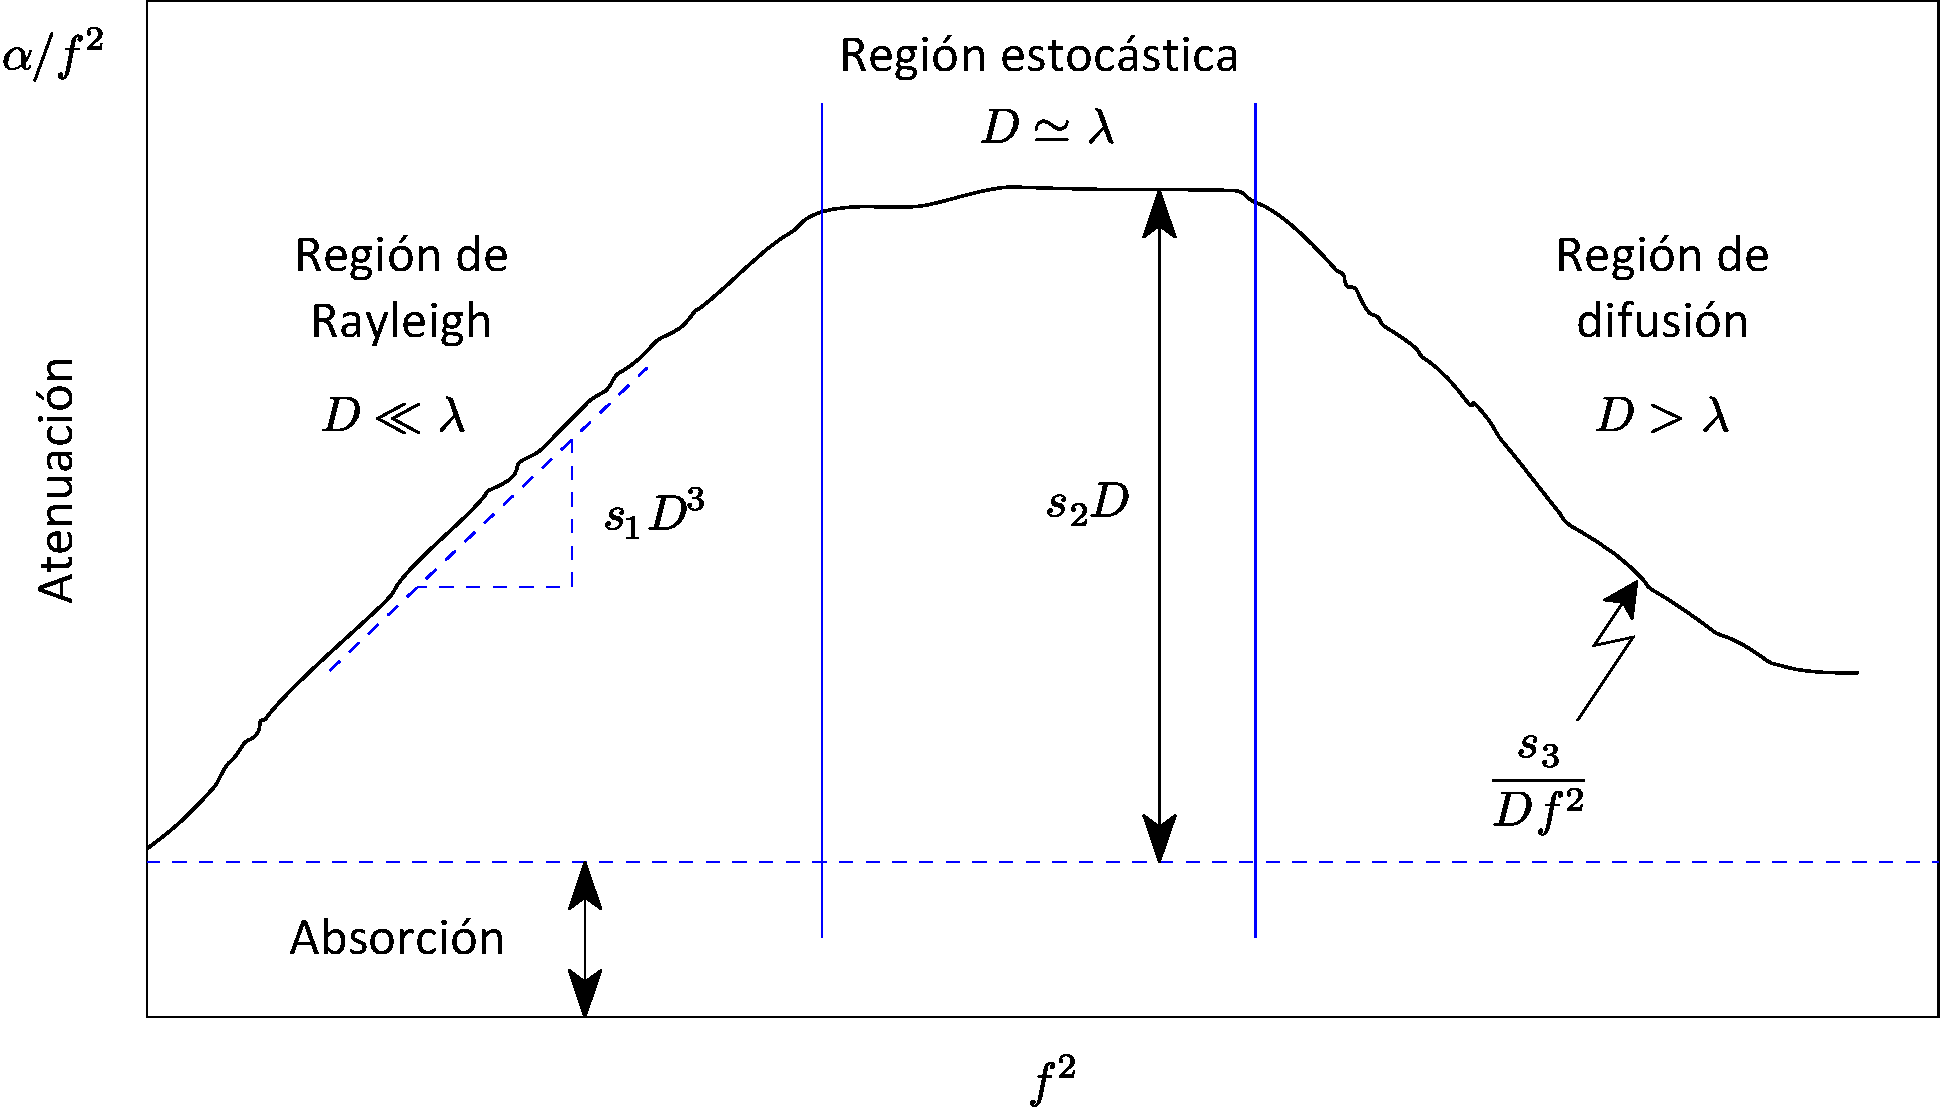
\includegraphics{gis-pfc-ch3-6.pdf}
	\end{center}
	\caption{Representaci�n del coeficiente de atenuaci�n que muestra su comportamiento en las distintas regiones del material}
	\label{fig:losscoefficient}
\end{figure}

Para finalizar este apartado, en la figura \vref{fig:losscoefficient} se muestra una representaci�n del coeficiente de atenuaci�n, en concreto del cociente $\alpha/f^2$, con respecto al cuadrado de la frecuencia. En la gr�fica es posible apreciar el comportamiento del coeficiente de dispersi�n en cada una de las regiones descritas, y como el t�rmino que introduce la absorci�n es de valor constante con la frecuencia. La regi�n de difusi�n muestra una atenuaci�n abrupta que responde a una exponencial decreciente descrita por la expresi�n $s_3/(Df^2)$.


\subsubsection{Limitaciones impuestas por la dispersi�n en los ensayos ultras�nicos}

La dispersi�n, que contribuye de dos modos distintos a perjudicar el proceso de inspecci�n ultras�nica, por un lado atenuando la se�al ac�stica, por otro lado causando el ruido de grano, es el principal factor limitante en los ensayos no destructivos. Es habitual que la dispersi�n limite la profundidad de una inspecci�n a la regi�n de Rayleigh.\par
Cualquier material posee granos de diferentes tama�os y, por tanto, un frente de ondas ac�sticas que atraviesa un material se ve afectado por la dispersi�n como si se encontrase en las tres regiones de dispersi�n descritas. No obstante, es el grano de mayor tama�o el que en la pr�ctica determina el comportamiento del material en t�rminos de dispersi�n.\par
La dispersi�n, debido a que es el causante del ruido estructural, no puede contrarrestarse aumentando la potencia de la onda ultras�nica en emisi�n. La soluci�n primera para evitar la dispersi�n pasa por disminuir la frecuencia de la onda, pero esto desemboca tambi�n en una p�rdida de resoluci�n. La mejor alternativa consiste en emplear t�cnicas de procesamiento de se�al que reduzcan la energ�a del ruido estructural en recepci�n.


\subsection{Algoritmos utilizados para la reducci�n del ruido estructural}

Dejando a un lado las t�cnicas empleadas en la eliminaci�n de ruido incoherente aleatorio, ineficaces por completo contra el ruido estructural, existe un conjunto de m�todos orientados a combatir este tipo de ruido.\par
Las t�cnicas empleadas con mayor frecuencia con el objeto de conseguir mayor \sig{snr} en entornos en los que la presencia de ruido estructural es notable son aquellas que aprovechan la diversidad de informaci�n hallada al trabajar con se�ales incorreladas entre s�. Estas t�cnicas tratan de obtener una se�al con una mayor \sig{snr} a partir de la composici�n de varias se�ales generadas mediante un mismo mecanismo pero de forma que la medida de correlaci�n entre cada una de ellas sea pobre. Los m�todos empleados m�s a menudo con tal prop�sito son:

\begin{itemize}
	\item Las t�cnicas que explotan la diversidad espacial, en las que b�sicamente se repite el mismo experimento variando cada vez la orientaci�n de los transductores implicados en el mismo.
	\item Y las t�cnicas de diversidad frecuencial, manteniendo la posici�n de los transductores se repite el experimento utilizando se�ales situadas en una banda espectral diferente unas de otras.
\end{itemize}

Este tipo de t�cnicas consiguen mejorar de forma considerable la \sig{snr} en inspecciones ultras�nicas, no obstante presentan una serie de inconvenientes que las hacen inapropiadas en determinadas situaciones. Por un lado, las t�cnicas de diversidad espacial se ven obstaculizadas con frecuencia por las dimensiones y forma de las piezas evaluadas, siendo en ocasiones imposible emplearlas. En cuanto a las t�cnicas de diversidad en frecuencia, los transductores empleados en inspecciones ultras�nicas act�an por lo com�n en una banda no lo bastante ancha como para poder dividirla en un gran n�mero de subbandas y as� poder emitir suficientes se�ales ac�sticas repartidas por el espectro de frecuencias. Para poder emplear una t�cnica as� ser�an necesarios varios transductores que emitiesen en bandas de frecuencia se�ales ac�sticas con ancho de banda controlado y que todos estuviesen situados en la misma posici�n.\par
La dificultad que conlleva implementar las t�cnicas anteriormente descritas ha contribuido a la proliferaci�n de t�cnicas que a partir de una �nica traza sacan partido de las diferencias estad�sticas que existen entre la se�al que procede de un defecto y el ruido estructural.\par
Dentro de esta categor�a el algoritmo que ha alcanzado un �xito mayor y en consecuencia se ha convertido en el paradigma de las t�cnicas de reducci�n de ruido estructural se conoce como t�cnica de partici�n espectral o del ingl�s \emph{Split Spectrum Processing} (\psig{ssp}) y fue en inicio propuesto por Vernon Newhouse en 1982. El algoritmo est� basado en la explotaci�n de la seudo"=diversidad frecuencial que existe entre las diferentes trazas de banda estrecha que se obtienen al descomponer con un banco de filtros paso banda la se�al resultante tras un ensayo. No obstante los excelentes resultados encontrados utilizando esta t�cnica, la gran sensibilidad que muestra el algoritmo a la sinton�a de los principales par�metros que definen su comportamiento lo convierten en escasamente robusto. A consecuencia de esto han aparecido numerosas publicaciones que se circunscriben a proporcionar configuraciones del algoritmo que proporcionen resultados �ptimos, alternativamente aparecen tambi�n variaciones del \sig{ssp} que persiguen mejorarlo.\par
A pesar de su �xito, el \sig{ssp} no es el �nico m�todo empleado con el objetivo de sustraer el ruido de grano de la se�al de inter�s de un \sig{endus}. Otros trabajos incluyen, la estimaci�n de m�xima verosimilitud, t�cnicas de filtrado paso"=banda que eliminan la mitad superior del espectro de la se�al, t�cnicas tiempo"=frecuencia como son la transformada de Wigner"=Ville o las Wavelet, t�cnicas que sacan partido de la informaci�n que aporta el retardo de grupo, t�cnicas no lineales y, finalmente, t�cnicas de ruido residual.\par
A pesar del gran n�mero de t�cnicas dedicadas a eliminar el ruido estructural, son pocos los trabajos orientados a establecer una relaci�n entre ellas, a compararlas, a clasificarlas seg�n su comportamiento en distintos tipos de materiales o a justificar por qu� el uso de una u otra t�cnica.


\section{T�cnicas de procesado por partici�n del espectro}

Bajo el t�rmino <<t�cnicas de procesado por partici�n del espectro>>, en ingl�s \emph{Split Spectrum Processing Techniques}, o simplemente \psig{ssp}, se re�nen una serie de algoritmos cuya aplicaci�n es la reducci�n del efecto del ruido estructural o de grano en los resultados de un \sig{endus}.\par
El principio en el que se fundamentan estas t�cnicas es similar al que rige las t�cnicas de diversidad convencionales. A partir de varias se�ales incorreladas entre s� se construye una se�al cuya \sig{snr} es considerablemente mejor que la \sig{snr} de cualquiera de las se�ales primitivas por separado. Las t�cnicas de \sig{ssp}, a diferencia de las t�cnicas basadas en la diversidad, consiguen s�lo una seudo"=diversidad en frecuencia a partir de una �nica traza de la se�al que se obtiene tras un \sig{endus}.\par
Con frecuencia se obtienen buenos resultados empleando estas t�cnicas lo que, sumado a la sencillez con la que puede implementarse un experimento fundamentado en las mismas, recordando que no es requerida una redundancia real basada en la utilizaci�n de varias se�ales, las ha convertido en las t�cnicas m�s populares en el �mbito de los \sig{endus}. A consecuencia de la reputaci�n con la que se han visto revestidas recientemente numerosas investigaciones se han llevado a cabo en las d�cadas de los ochenta y los noventa, as� como a principios de siglo, con el fin de mejorar en la medida de lo posible los buenos resultados que ya de por s� proporcionan las t�cnicas de \sig{ssp}.\par
El procedimiento (m�s detallado en el \ref{tab:sspfeatures}) que por lo general sigue todo el conjunto de t�cnicas de \sig{ssp} consiste en aplicar una transformaci�n sobre la traza que comprende dos pasos:

\begin{itemize}
	\item El primero, dividir la traza en un n�mero determinado de se�ales de banda estrecha, para lo que se emplea un banco de filtros.
	\item En segundo lugar se reconstruye la traza, o m�s bien una versi�n de �sta con una \sig{snr} mejorada, mediante un algoritmo de reconstrucci�n no lineal.
\end{itemize}

Las diferencias entre el car�cter estad�stico del ruido y de la se�al procedente del defecto hacen que el procedimiento anterior conduzca al resultado deseado. Para concretar, la distribuci�n de la energ�a del ruido no es equitativa en frecuencia, de ah� que sea posible encontrar se�ales incorreladas en ruido mediante la divisi�n espectral que realiza el banco de filtros. Por otro lado, la linealidad que presenta la componente de la se�al ---o alteraci�n de la misma seg�n sea el caso--- originada en la reflexi�n que se produce al encontrarse la onda ac�stica con el defecto conlleva que la muestra que identifica la presencia del defecto se encuentra en la misma posici�n en todas las trazas de banda estrecha. Los m�todos de \sig{ssp} aprovechan de manera impl�cita esta �ltima caracter�stica de la traza para magnificar la componente de la se�al que indica la presencia del defecto por lo que son catalogados en la bibliograf�a como m�todos que explotan la fase del defecto.\par

\begin{table}
	\centering
	\begin{tabulary}{.95\textwidth}{>{$(}c<{)$}Lr@{\hspace{6pt}}L}
		\toprule
		\multicolumn{2}{c}{Par�metros} & \multicolumn{2}{c}{Algoritmo} \\
		\cmidrule(r){1-2}\cmidrule(l){3-4}
		y & Se�al a procesar & 1. & Generar del banco de filtros \\
		f_\text{min} & Frecuencia inferior de corte del banco de filtros & 2. & Calcular la \sig{fft} de $y$ \\
		f_\text{max} & Frecuencia superior de corte del banco de filtros & 3. & Procesar el resultado obtenido en (2) con el banco de filtros \\
		\Delta f & Separaci�n entre filtros & 4. & Calcular la \sig{ifft} de las trazas de banda estrecha \\
		pb & Ancho de banda de los filtros & 5. & Normalizar la amplitud de las trazas de banda estrecha \\
		h_f & Tipo de filtro empleado & 6. & Construir una �nica traza a partir de las trazas de banda estrecha normalizadas \\
		\bottomrule
	\end{tabulary}
	\caption{Particularidades que en general se aplican a todos los algoritmos de \sig{ssp}}
	\label{tab:sspfeatures}
\end{table}

\begin{figure}
	\begin{center}
		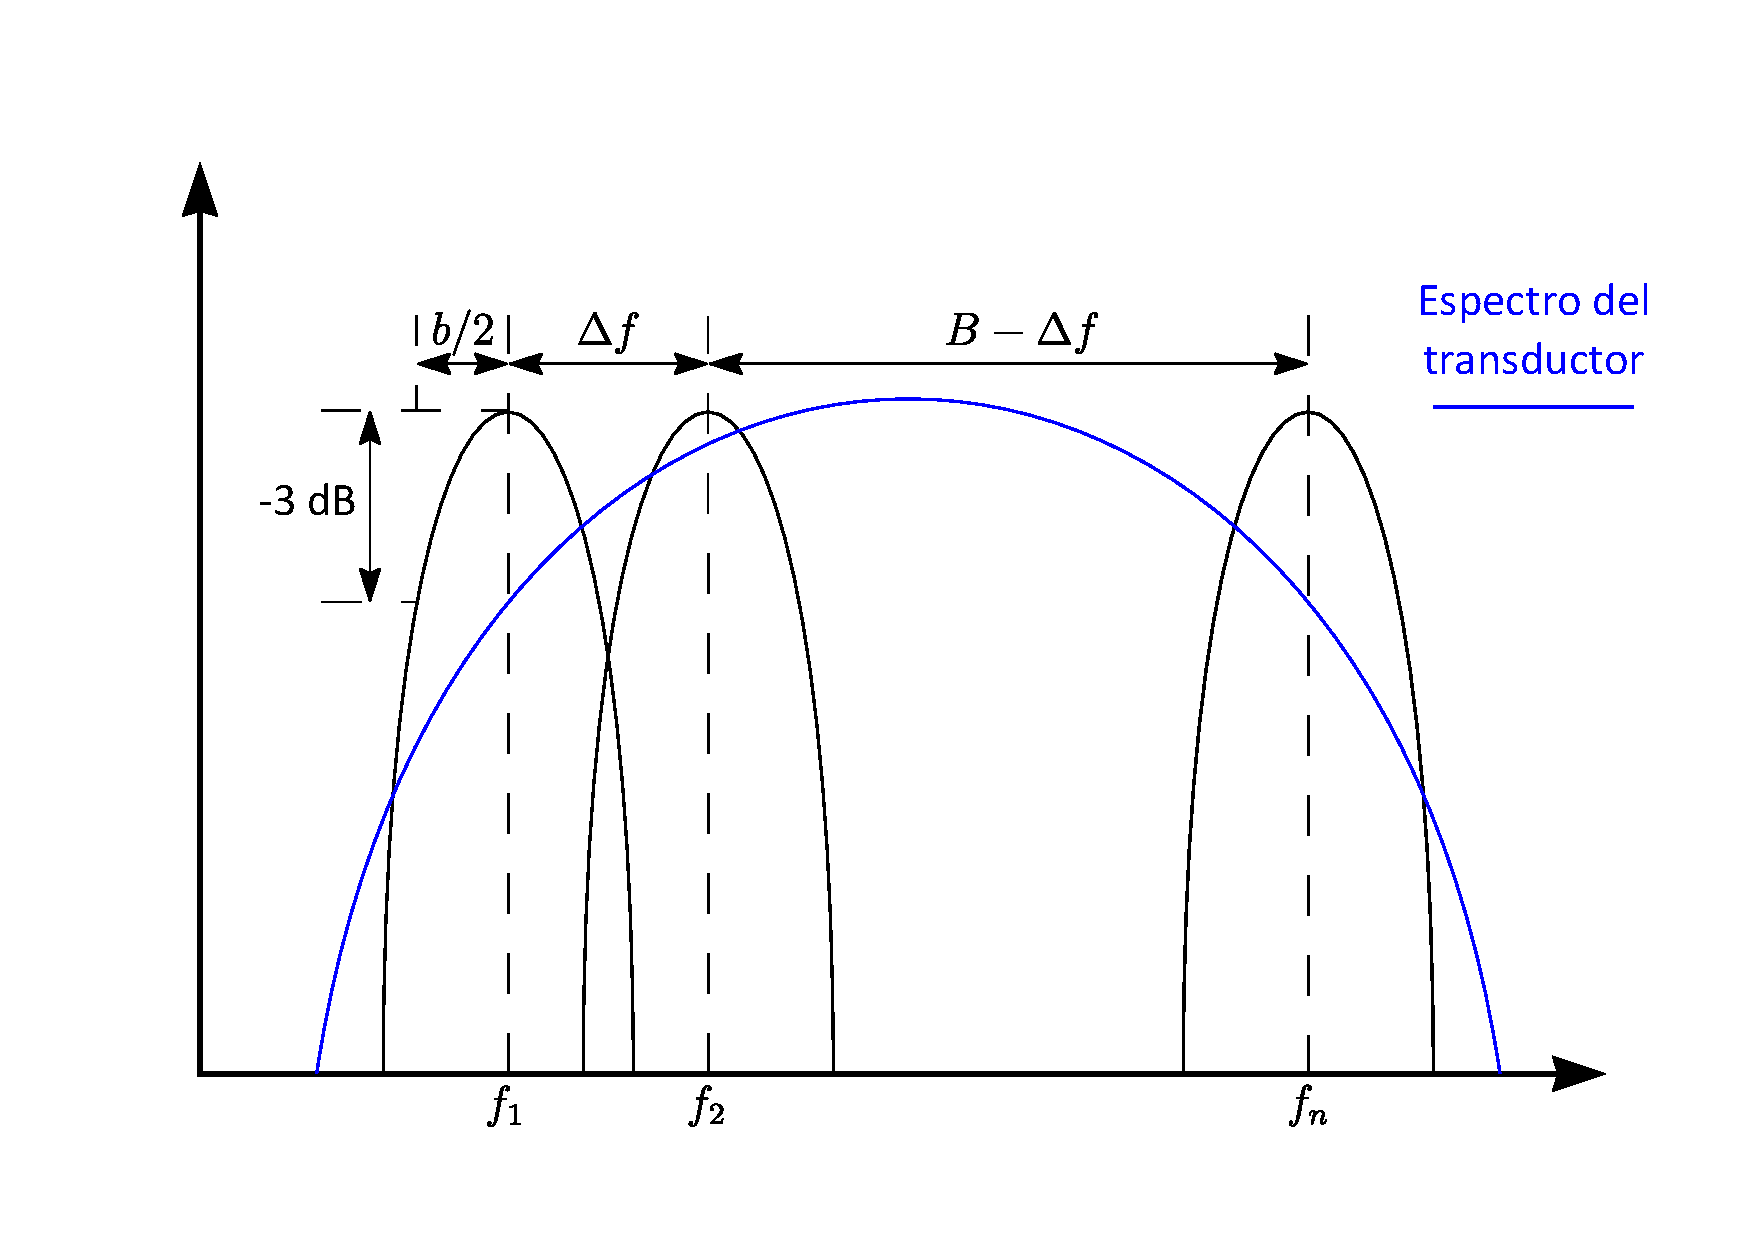
\includegraphics{gis-pfc-ch3-7.mps}
	\end{center}
	\caption[Par�metros de configuraci�n del banco de filtros]{Representaci�n esquem�tica en la que pueden observarse los par�metros empleados en la configuraci�n del banco de filtros comparados con el espectro de la se�al de audio}
	\label{fig:filter}
\end{figure}

% He hecho un corte del fichero aqu� porque el realzado de sintaxis de Vim no interpreta correctamente el c�digo que configura la disposici�n de las columnas en el entorno tabulado etiquetado con <<tab:sspfeatures>>, en consecuencia considera todo el texto posterior incluido en una ecuaci�n matem�tica y no resalta la ortograf�a.
La eficacia de las t�cnicas de \sig{ssp} no est� garantizada, depende en gran parte de dos de los par�metros listados en el \cref{tab:sspfeatures}.

\begin{itemize}
	\item Por un lado est� la configuraci�n del banco de filtros, a destacar dos aspectos:
		\begin{itemize}
			\item El tipo de filtro empleado. Seg�n afirma M.\,A. Izquierdo en (\cite{garcia2000mrsr}), trabajos realizados a principios de los noventa como los de P.\,Karpur apuntan a la existencia de una relaci�n entre el factor de forma de los filtros que se utilizan para realizar la partici�n de espectro y la bondad de los resultados aportados por la t�cnica de \sig{ssp}. Se�ala M.\,A. Izquierdo que, a pesar de que la influencia que ejerce este par�metro en la calidad del ensayo haya mostrado ser notable, estudios posteriores no han tenido en cuenta las conclusiones alcanzadas por Karpur.
			\item La zona del espectro en la que se aplica el m�todo. La regi�n del espectro que queda bajo el banco de filtros puede configurarse ajustando las frecuencias de corte superior e inferior del banco ---quedando indirectamente condicionados el ancho de banda de los filtros y la separaci�n entre los mismos---. Es importante evitar que la banda de paso del banco coincida con alguna porci�n de la se�al en la que la informaci�n espectral que indica la presencia del defecto quede enmascarada por el ruido de grano. Cuando as� ocurre la efectividad del m�todo se reduce en gran medida.
		\end{itemize}
	\item El par�metro que resta por considerar no es otro que el algoritmo de reconstrucci�n que permite recuperar la traza definitiva. Las t�cnicas de \sig{ssp} se basan en la estabilidad de la fase de ah� su precaria robustez. El algoritmo de reconstrucci�n empleado es un factor determinante del que depende en gran parte la robustez de la t�cnica. Por tanto, aplicar un algoritmo de reconstrucci�n adecuado a las muestras es crucial para obtener buenos resultados. Los algoritmos m�s empleados son el de m�nimo del ensamble y el del umbral de polaridad (\emph{Polarity Thresholding}) o combinaci�n de ambos, a continuaci�n se citan otros.
\end{itemize}

Los trabajos mencionados en este apartado siguen todos una misma l�nea de investigaci�n, descubrir qu� configuraci�n del banco de filtros y qu� m�todo de reconstrucci�n optimizan los resultados de aplicar las t�cnicas de \sig{ssp} en un \sig{endus}. Se ha dicho que el t�rmino \sig{ssp} agrupa a un conjunto de t�cnicas, lo que las diferencia precisamente es, o bien el algoritmo de reconstrucci�n que emplean, o bien la forma en la que se configura el banco de filtros, en ocasiones ambos.\par
En cuanto a la configuraci�n del banco de filtros, algunos trabajos, es especial algunos de Karpur, aportan avances significativos. El autor encuentra para el algoritmo de m�nimos, de forma anal�tica y apoy�ndose en un modelo estacionario del ruido de grano, los par�metros que optimizan el rendimiento de la t�cnica de \sig{ssp}. Los valores hallados son los siguientes:

\begin{equation}
	\begin{split}
		N & = B\cdot T_y + 1 \\	
		b & = \Delta f = \frac{1}{T_y}
	\end{split}
\end{equation}

Donde $N$ representa el n�mero �ptimo de filtros, $B$ el ancho de banda del transductor en el segmento de recepci�n, $T_y$ la duraci�n de la se�al recibida, $b$ el ancho de banda de cada filtro, y $\Delta f$ la separaci�n entre filtros.\par
Por otro lado Karpur afirma en otro de sus estudios, esta vez apoy�ndose en la expresi�n para la atenuaci�n en la regi�n de Rayleigh, que el banco de filtros debe aplicarse en las frecuencias m�s bajas del espectro de la se�al, ya que es en esa zona en la que se concentra la mayor parte de la energ�a correspondiente a la radiaci�n que tiene origen en el defecto.\par
Otros estudios utilizan la informaci�n relativa a la distribuci�n espectral de la \sig{snr}, obtenida mediante algoritmos como el del histograma espectral o a partir de estad�sticos del retardo de grupo como p.e. la entrop�a m�vil, para determinar cu�l es la regi�n del espectro de la se�al en la que es �ptimo aplicar el filtrado.\par
En cuanto a los algoritmos de reconstrucci�n J.\,Saniie llega a la conclusi�n, en su trabajo de 1991 en el que estudia los filtros de orden aplicados como algoritmos de composici�n, de que los mejores resultados se obtienen cuando la se�al proviniente del defecto y el ruido estructural est�n estad�sticamente separados en un determinado cuantil. Dependiendo de las distribuciones de probabilidad del ruido y del defecto, resulta apropiado emplear algoritmos de m�nimos, mediana o m�ximos del ensamble, aunque por lo general el algoritmo de m�nimos es el que mejores resultados proporciona.\par
Por su parte M.\,G.\,Gustafsson propone una variante en el conjunto de las t�cnicas de \sig{ssp} en la que, bas�ndose en la teor�a bayesiana de detecci�n y a partir de la informaci�n de la se�al y el ruido coherente, pueden encontrarse todos los par�metros necesarios para aplicar la t�cnica de \sig{ssp}. El nombre que recibe usualmente esta variante es t�cnica de \sig{ssp} con detecci�n �ptima.


\section{Dise�o del instrumento de medida}

Esta secci�n est� dedicada al proceso de dise�o que se lleva a cabo para implementar mediante los recursos disponibles la instrumentaci�n electr�nica que junto con la tarjeta de adquisici�n y el software de control forman parte del aparato empleado en las mediciones efectuadas durante este proyecto fin de carrera.\par
En apartados posteriores se observa que este primer dise�o carece de las propiedades requeridas en los experimentos programados, pero igualmente se ha decidido incorporar a la memoria las notas correspondientes a esta fase del proyecto por considerar que al tratar una disciplina distinta con respecto al resto del documento \mbox{---dise�o} e implementaci�n de instrumentaci�n electr�nica--- enriquecen el contenido del mismo.


\subsection{Tipos de ensayo programados}

Es la naturaleza de los experimentos la que dictamina cuales deben ser las caracter�sticas del instrumento de medida. Sin olvidar el prop�sito primero de este proyecto ---determinar un m�todo efectivo para la detecci�n de defectos en madera de palmera empleando para ello ensayos no destructivos con se�ales de ultrasonidos--- se programan dos tipos de prueba:

\begin{itemize}
	\item Por un lado, pruebas de laboratorio con madera de palmera talada y preparada.
	\item Por otro, pruebas de campo con palmeras en un entorno natural, no siendo necesario que las palmeras sean silvestres, pudiendo encontrarse plantadas en un jard�n o espacio similar.
\end{itemize}

Se escoge la t�cnica de transmisi�n, en defecto de la t�cnica de pulso"=eco, para la realizaci�n de los ensayos. El equipo disponible al inicio del trabajo experimental var�a en funci�n de la prueba: para los experimentos de laboratorio se cuenta con un sistema de adquisici�n como el conformado por el conjunto de la tarjeta de adquisici�n, un ordenador, el software de control y la caja de conexiones; y para las pruebas de campo con un osciloscopio y una fuente de alimentaci�n, ambos alimentados con una bater�a. En ambos tipos de prueba deben emplearse tambi�n dos transductores, uno en transmisi�n y otro en recepci�n, junto con sus respectivos circuitos acondicionadores.


\subsection{Requisitos del instrumento de medida}

Para justificar cuales son los requisitos aplicables a los transductores y a las etapas acondicionadoras que los preceden, se recuerda aqu� de forma resumida al lector una serie de conclusiones a las que se ha llegado a lo largo de la secci�n anterior (la \cref{sec:theory} con inicio en la \vpageref{sec:theory}).\par
Los tres par�metros cruciales en el desempe�o de un \sig{endus} son: la resoluci�n, tanto axial como lateral; la profundidad de penetraci�n; y la relaci�n se�al a ruido.

\begin{itemize}
	\item La resoluci�n viene determinada principalmente por el tama�o y el tipo de transductores empleados. Cuanto mayor sea el ancho de banda de los transductores y menores sus dimensiones, se alcanzar�n mejores resoluciones. Asimismo, una buena resoluci�n depende de la forma y frecuencia de los pulsos ultras�nicos, siendo mejor cuanto m�s estrecho sea el pulso y mayor su frecuencia.
	\item La profundidad de penetraci�n, factor determinante en los experimentos realizados para este proyecto, depende fundamentalmente de la potencia transmitida en cada pulso y de su frecuencia de oscilaci�n, siendo mayor cuanto mayor sean estos dos par�metros.
	\item Sin embargo, la consecuci�n de una buena relaci�n se�al a ruido est� re�ida con una buena profundidad de penetraci�n. El ruido estructural, principal factor limitante de la relaci�n se�al a ruido, se agrava a medida que aumenta la frecuencia o la potencia del pulso ultras�nico. Para poder realizar ensayos capaces de detectar defectos en el medio a profundidades razonables sin sufrir en exceso los efectos del ruido de grano es determinante aplicar un buen algoritmo para la reducci�n del ruido.
\end{itemize}

Por supuesto, la calidad de un ensayo exige buenas configuraciones de estos tres par�metros. Sin embargo, y dado que los ensayos realizados para el proyecto no requieren la detecci�n precisa del defecto, si no s�lo su detecci�n, una buena resoluci�n no ser�a exigible aunque s� deseable. Por el contrario, el material objeto de este estudio es la madera de palmera, puesto que desde la planificaci�n del proyecto se preven pruebas de campo en palmeras vivas, y adem�s se opta por emplear la t�cnica de transmisi�n (l�ase el \cref{subsec:technics}), resulta imprescindible trabajar con una buena profundidad de penetraci�n, de forma que la se�al de ultrasonidos sea capaz, al menos, de atravesar el tronco de las palmeras.\par
En base a los requisitos establecidos por las caracter�sticas de los ensayos se extraen las necesidades de potencia y frecuencia que deben cubrir los transductores y los circuitos acondicionadores, as� como el resto de instrumentos utilizados.\par


\paragraph{Requisitos de frecuencia.}

La frecuencia de las se�ales ultras�nicas empleadas en ensayos no destructivos oscila generalmente entre los 20 kHz y los 25 MHz. Sin embargo, existen l�mites pr�cticos que impiden trabajar en un rango de frecuencias tan amplio. En primer lugar, el precio de los transductores aumenta significativamente a medida que aumenta su ancho de banda, la posibilidad de emitir pulsos de alta frecuencia tambi�n encarece el precio de estos dispositivos\footnote{Es habitual encontrar sensores que trabajan a frecuencias entorno a los 40 kHz por un precio entorno a las \mbox{5 \pounds{}}, mientras que sensores que funcionan a 300 kHz pueden costar aproximadamente unas \mbox{300 \pounds{}} (referencia extra�da de la p�gina web \href{http://uk.farnell.com}{uk.farnell.com})}. Por otro lado, la banda de paso de las etapas de acondicionamiento, la frecuencia m�xima obtenible de la fuente de alimentaci�n, y la frecuencia de muestreo m�xima del instrumento de adquisici�n, limitan la frecuencia de la se�al de ultrasonidos. \par
Obviamente, es el l�mite m�s restrictivo el que se aplica. En este caso, el l�mite m�s restrictivo lo imponen los transductores y la tarjeta de adquisici�n. Los transductores a los que se ha tenido acceso en el desarrollo del proyecto son de bajo coste y su frecuencia de oscilaci�n natural se ubica en los 40 kHz, podr�a decirse que en el l�mite inferior de la banda de frecuencias empleada en los \sig{endus}. Por su parte, la tarjeta de adquisici�n ofrece en condiciones �ptimas una tasa de muestreo de 100 KS/s. Lo que implica que, para su correcta visualizaci�n en el dispositivo de adquisici�n empleado en el laboratorio, la frecuencia de la se�al anal�gica que se muestrea debe encontrarse alrededor de los 20 kHz.\par
Quiz� el lector haya advertido que esta relaci�n ---frecuencia de muestreo unas cinco veces superior a la frecuencia de la se�al anal�gica--- supera con creces lo establecido por el teorema de Nyquist, $f_s = 2\Delta f$. Esto es debido a que el objetivo del muestreo es visualizar en el monitor del ordenador la forma de la se�al a partir de la reconstrucci�n que \matlab{} hace de las muestras. Al contrario de lo que ocurre con el teorema de Nyquist"=Shannon, que determina la frecuencia de muestreo m�nima para que una se�al anal�gica pueda ser recuperada a partir de sus muestras no cuantificadas sin p�rdida de informaci�n, para percibir la forma de una se�al en una reconstrucci�n arbitraria de la misma realizada partiendo de sus muestras cuantificadas la frecuencia de muestreo necesaria debe ser muy superior a la indicada por el teorema.


\paragraph{Requisitos de potencia.}

Puesto que la frecuencia de oscilaci�n de los pulsos ultras�nicos est� limitada a los 40 kHz por los motivos pr�cticos citados en el apartado anterior, y dada la necesidad de una profundidad de penetraci�n notable, los requisitos en cuanto a la potencia que debe manejarse en las etapas de transmisi�n y recepci�n se encuentran muy restringidos.\par
Para suplir las carencias que los transductores tienen en frecuencia es l�gico recurrir a se�ales de mayor potencia, sin embargo el precio reducido de los dispositivos empleados tambi�n limita su capacidad de emitir se�ales de alta potencia.\par
Lo que en �ltima instancia significa que, con ninguna de las posibles soluciones al alcance del proyecto puede obtenerse la profundidad de penetraci�n adecuada para el tipo de experimentos que se desea realizar. L�ase a continuaci�n, en la \vpageref{subsec:solution}, la soluci�n finalmente adoptada y la valoraci�n preliminar que el autor hace con antelaci�n a la fase de dise�o.


\subsection{Recursos disponibles al inicio de la etapa de dise�o}

Para la implementaci�n del instrumental electr�nico se dispone inicialmente de dos transductores ultras�nicos, uno destinado a funcionar como transistor y otro que realiza el papel de receptor. Ambos transductores manufacturados por el mismo fabricante y de una misma gama, con caracter�sticas similares. En el \vref{tab:transducers} se muestran las principales propiedades de ambos transductores.\par
Adem�s, el fabricante proporciona en la ficha t�cnica la respuesta caracter�stica del transmisor a un pulso rectangular. La curva, que puede observarse en la \cref{fig:response}, se asemeja a un pulso gaussiano que modula a una sinusoide de frecuencia igual a la frecuencia de resonancia del transductor. Esta respuesta a se�ales pulsadas de pulsos rectangulares hace que este tipo de transductor sea muy apropiado para su uso en \sig{endus}.\par
En cuanto a su aspecto y dimensiones, los transductores se encuentran protegidos por un encapsulado pl�stico de color negro, pudiendo distinguir el transmisor gracias a un punto blanco situado en la pared exterior del encapsulado. Las dimensiones de los dos transductores coinciden, y son las mostradas en la figura esquem�tica \ref{fig:transducer}.

\begin{table}
	\centering
	\begin{threeparttable}
		\begin{tabular}{l c c}
			\toprule
			& \multicolumn{2}{c}{Transductor} \\
			\cmidrule(l){2-3}
			Propiedad & Transmisor & Receptor \\
			\midrule
			Sensibilidad en transmisi�n\tnote{a} & 110 dB & -- \\
			Sensibilidad en recepci�n\tnote{b} & -- & -70 dB \\
			Frecuencia de resonancia (kHz) & $40 \pm 1$ & $40 \pm 1$ \\
			Ancho del l�bulo principal & 60\,� & -- \\
			Tensi�n de alimentaci�n m�xima\tnote{c} & 10 Vef & -- \\
			M�xima potencia admitida\tnote{d} & 200 m\!Wef & \\
			Impedancia\tnote{e} & $700\ \Omega$ & $30\ \text{k}\Omega$ \\
			Capacidad (nF) & $2 \pm 20\%$ & $2 \pm 20\%$ \\
			Tiempo de subida del pulso & $700\ \mu\text{s}$ & -- \\
			Tensi�n m�xima admitida en modo pulsado & 20 V & -- \\
			Rango de temperatura de funcionamiento (�C) & (-20, 60) & (-20, 60) \\
			\bottomrule
		\end{tabular}
		\begin{TableNotes}
			\tnotetext{a}{Decibelios medidos con respecto a una referencia de 200 nbar a 30 cm cuando el transmisor se alimenta con una tensi�n eficaz de 10 Vef.}
			\tnotetext{b}{Decibelios medidos con respecto a una referencia de 1 V/$\mu\text{bar}$.}
			\tnotetext{c}{Esta es la tensi�n m�xima que el transductor admite cuando se alimenta de forma continuada con una se�al de alterna.}
% 			\tnotetext{d}{Se emplea en este documento el s�mbolo Vef como sin�nimo de la unidad de potencial el�ctrico en corriente alterna, \emph{voltios eficaces}. Del mismo modo se utiliza Wef, \emph{vatios eficaces}, como unidad de potencia eficaz.}
			\tnotetext{d}{Se refiere a la potencia m�xima que el transductor puede disipar en modo pulsado, es decir, cuando la alimentaci�n es interrumpida y peri�dica.}
			\tnotetext{e}{En transmisi�n esta magnitud representa la impedancia de entrada equivalente del transductor. En recepci�n, por el contrario, representa la impedancia de salida del transductor.}
		\end{TableNotes}
	\end{threeparttable}
	\caption[Caracter�sticas de los transductores empleados en el dispositivo de medida]{Caracter�sticas de los transductores empleados en el dispositivo de medida (se proporcionan los valores t�picos para cada propiedad).}
	\label{tab:transducers}
\end{table}

\begin{figure}
	\begin{center}
		\includegraphics{gis-pfc-ch3-01.mps}
	\end{center}
	\caption[Respuesta del transmisor a un pulso rectangular]{Respuesta del transmisor a un pulso rectangular.}
	\label{fig:response}
\end{figure}

\begin{figure}
	\begin{center}
		\includegraphics{gis-pfc-ch3-01.mps}
	\end{center}
	\caption[Dimensiones de los transductores de ultrasonidos]{Dimensiones de los transductores de ultrasonidos.}
	\label{fig:transducer}
\end{figure}

El resto de componentes empleados en la implementaci�n de las etapas de acondicionamiento se encontraban disponibles en el laboratorio de teor�a de la se�al en el que esta tarea se lleva a cabo. Entre ellos cabe destacar el \sig{TL}082, un amplificador operacional de prop�sito general cuyas prestaciones superan ampliamente a las ofrecidas por el cl�sico \AOUA{} en t�rminos de banda de frecuencias amplificada. Mientras que el \AOUA{} convencional mantiene su m�xima ganancia para se�ales de entrada de frecuencia alrededor de los 7 kHz, el amplificador empleado consigue amplificar con su m�ximo factor de ganancia se�ales que oscilan con frecuencias m�ximas de 90 kHz. Es imprescindible disponer de un amplificador que conserve su ganancia por encima de los 40 kHz, ya que esta es la frecuencia de resonancia de los transductores, y la frecuencia de trabajo seleccionada para el dispositivo de medida.


\subsection{Soluci�n adoptada}\label{subsec:solution}


\subsubsection{Valoraci�n preliminar}

A la vista de los requisitos que exige una aplicaci�n como la propuesta en este proyecto, las necesidades que surgen durante su dise�o y los medios y recursos disponibles, parece previsible un fracaso en el desarrollo de la parte experimental de este \sig{pfc}. Pese a todo, y puesto que el coste de implementar los circuitos y realizar las pruebas es en la pr�ctica suficientemente reducido, se decide proseguir con los experimentos ya que el verdadero fin del proyecto es obtener una serie de resultados, sean estos los esperados o no, y de estos deducir una serie de conclusiones.\par
En el momento en el que se desarrolla esta fase del proyecto se contempla la posibilidad de inferir dos conclusiones distintas a partir de los resultados: si los resultados no son buenos, determinar cu�les son en realidad los requisitos que deben cumplirse para poder aplicar los \sig{endus} de manera efectiva en la detecci�n de defectos en madera de palmera, y sabiendo esto justificar la ausencia de resultados v�lidos; y, en el caso contrario, en caso de que los resultados fueran satisfactorios, verificar la validez de aplicar este m�todo con un mismo prop�sito y en unas condiciones similares.\par
Posteriormente, tal como se relata en la {\color{red}secci�n ??} se tiene acceso a unos transductores distintos, que por su modo de funcionamiento permiten llevar a cabo de modo satisfactorio las pruebas programadas.


\subsubsection{Montaje seleccionado}

En vista de las conclusiones extra�das en apartados anteriores, y teniendo en cuenta las soluciones a las que se tiene acceso, con el prop�sito de obtener los mejores resultados posibles, se opta por un montaje que exprime al m�ximo el transmisor y que en la secci�n de recepci�n utiliza un amplificador de instrumentaci�n cuyo factor de ganancia es muy elevado.\par % Para ello, de las soluciones a las que se tiene acceso
Esta soluci�n, que en una primera instancia parece adecuada, presenta no obstante importantes inconvenientes, de entre los cuales destaca la baja calidad de relaci�n se�al a ruido que proporciona.\par
En principio, el uso de se�ales de elevada potencia que oscilan a bajas frecuencias es propicio para evitar las complicaciones que en un ensayo introduce el ruido de grano. Si bien la se�al que emite el transductor de la secci�n de transmisi�n no es de una potencia considerable, las bajas frecuencias a las que oscila garantizan que se consiga en parte este objetivo.\par
No obstante no es el ruido de grano el m�s perjudicial en esta configuraci�n. Los transductores de ultrasonidos son transductores piezoel�ctricos y, por tanto, el sensor empleado en recepci�n se engloba en la categor�a de los sensores generadores. Es decir, que en respuesta a una actividad ultras�nica genera una determinada se�al el�ctrica. La frecuencia y amplitud de la se�al el�ctrica que proporciona el sensor dependen de la se�al ac�stica detectada. Y, si como ocurre en este caso, la se�al ultras�nica que alcanza el sensor es muy tenue, la se�al el�ctrica correspondiente muestra un recorrido de tensi�n muy reducido. De tal forma que incluso puede ser comparable al ruido presente a la entrada del circuito de adquisici�n o a otras se�ales indeseadas.\par
Por consiguiente, es, en la secci�n de recepci�n, el ruido electr�nico procedente de la etapa de acondicionamiento el m�s significativo y el de m�s dif�cil soluci�n. Por tres razones que se detallan a continuaci�n.

\begin{itemize}
	\item En primer lugar, debido a que la procedencia del ruido nada tiene que ver con la interacci�n de la se�al ac�stica con el medio, las t�cnicas de postprocesado cuyo objetivo es eliminar el ruido procedente del entorno no son aplicables.
	\item En principio, es posible aplicar las t�cnicas destinadas a reducir la presencia de ruido gaussiano vistas en el \cref{subsec:noise}. Sin embargo, con dificultad pueden obtenerse mejoras aceptables de la \sig{snr} en circunstancias como las aqu� expuestas.
	\item Otra posible soluci�n podr�a encontrarse al abordar el problema desde el prisma de la teor�a de la instrumentaci�n electr�nica. Esta teor�a ha mostrado ser eficaz resolviendo problemas similares en el acondicionamiento de sensores de m�ltiples tipos. Pueden citarse como ejemplo: el uso del puente de Wheatstone en el acondicionamiento de sensores resistivos, circuito que elimina la componente de se�al invariante que introduce el divisor de tensi�n; o la utilizaci�n de c�lulas isotermas y fuentes de corriente dependientes de la temperatura para eliminar la componente de se�al que generan las uniones de un termopar con los cables de medida.\par
		No obstante dadas las caracter�sticas del sensor y de la se�al que genera, la aplicaci�n de una soluci�n semejante es ciertamente dif�cil.
\end{itemize}


\subsection{Dise�o de la etapa de transmisi�n} % {Requisitos concretos aplicables a la etapa de acondicionamiento en transmisi�n} % [Requisitos de la etapa de transmisi�n]

El prop�sito del circuito acondicionador de la etapa de transmisi�n es proporcionar una se�al de alimentaci�n que se ajuste a las limitaciones del transductor y a los requisitos especificados en la etapa anterior de la fase de dise�o.


\subsubsection{La se�al de alimentaci�n}

Las especificaciones 
Los requisitos de la etapa de transmisi�n pueden obtenerse al juzgar por un lado los l�mites del transductor de ultrasonidos que se emplea como transmisor y por otro las especificaciones que debe cumplir la se�al ac�stica transmitida.\par
En \sig{endus}, la t�cnica de transmisi�n exige una se�al pulsada como la que proporciona el transmisor cuando es alimentado por un pulso rectangular. Por otro lado, una de las condiciones de dise�o consiste en emitir a la m�xima potencia posible. La se�al ac�stica es emitida por el transmisor de ultrasonidos, por consiguiente la potencia de esta se�al depende de los l�mites del transductor y de como se encuentra alimentado.\par
% Estoy hablando de las caracter�sticas de la se�al de alimentaci�n, porqu� no hacer una subsubsecci�n hablando del tema. Es decir, a partir de los datos que tengo razono como debe ser la se�al de alimentaci�n y luego digo como la implemento.
Consultando el \vref{tab:transducers} puede observarse que la m�xima potencia que puede disipar el transductor es de 200 m\!Wef en modo pulsado. Puesto que la impedancia de entrada t�pica interna del transductor es de $700\ \Omega$ pueden calcularse de forma sencilla valores para la potencia instant�nea y, a partir de este �ltimo dato, el nivel de tensi�n m�ximo con el que debe alimentarse el transductor. Para realizar estos c�lculos, primero debe fijarse otro par�metro: la forma de la se�al de alimentaci�n y sus caracter�sticas temporales.\par
% �Por qu� elijo una se�al pulsada? Porque as� se generan pulsos de forma autom�tica sin necesidad de presionar ning�n bot�n, ni realizar ninguna otra acci�n. Esto es bueno porque me ahorro interruptores que quiz� deban ser reemplazados en el futuro por perder parte de sus cualidades. El periodo con el que se generan los pulsos no deber�a ser demasiado corto, lo que impedir�a explotar al m�ximo el transductor, y debe permitirme seguir los cambios de se�al en el monitor del osciloscopio.
Resulta conveniente elegir una se�al pulsada para la alimentaci�n, en concreto un tren de pulsos rectangulares, dado el comportamiento del transductor frente a este tipo de pulsos. En cuanto al ciclo de trabajo por conveniencia se elige, respectivamente: la duraci�n del estado alto, 375 $\mu$s, equivalente a 15 periodos de la portadora; y una frecuencia de aproximadamente 1 Hz. % Una frecuencia tan baja permite un seguimiento visual de la se�al, de ese modo es posible congelar el osciloscopio manualmente y eso simplifica el proceso de medida.\par
% Consultando el \vref{tab:transducers} puede observarse que la m�xima tensi�n admitida por el transductor en modo pulsado es de 20 V, y la m�xima potencia que puede disipar es de 200 mW. Por lo tanto, la corriente de la se�al de alimentaci�n debe limitarse a 10 mA, algo que puede lograrse mediante una carga adicional. En cuanto a la duraci�n de los pulsos y el periodo de la se�al pulsada, por conveniencia se elige respectivamente un tiempo de 375 $\mu$s, equivalente a 15 periodos de la portadora, y una frecuencia de $1/4$ Hz. Una frecuencia tan baja permite un seguimiento visual de la se�al, de ese modo es posible disparar el osciloscopio manualmente y eso simplifica el proceso de medida.\par
% Consultando el \vref{tab:transducers} y la \cref{fig:response} puede deducirse cuales son las caracter�sticas de la se�al de alimentaci�n que debe proporcionar la etapa de acondicionamiento en transmisi�n. Al emplear la t�cnica de transmisi�n es necesario que la se�al que emite el transductor sea una se�al pulsada
En las pruebas de laboratorio basta con emplear el generador de se�ales y, si se requiere, un peque�o amplificador de ganancia moderada. Por ejemplo, el generador dispuesto para el proyecto proporciona una se�al con valor de pico a pico m�ximo de 10 voltios pico"=pico (en adelante Vpp), puesto que va a emplearse el transmisor en modo pulsado, la ganancia del amplificador debe ser de 2 V/V. Ganancia que puede obtenerse f�cilmente con un amplificador monoetapa basado en un amplificador operacional de prop�sito general.\par
Para las pruebas de campo se dise�a un circuito capaz de emitir una se�al pulsada, de pulsos rectangulares, que pueda ser alimentado con la misma fuente de alimentaci�n con la que es alimentado el acondicionador de la secci�n de recepci�n. De ese modo se evita el consumo extra que el generador de se�ales hace de la bater�a al mismo tiempo que se transporta un equipo menos. El circuito mencionado se basa en el temporizador integrado 555, concretamente en el integrado 556 que contiene dos 555 en un mismo encapsulado, y el amplificador de uso com�n \AOUA{}.\par
El 555 en su configuraci�n como multivibrador astable es capaz de producir una se�al peri�dica de pulsos rectangulares en los que la duraci�n del estado alto y del estado bajo ---y, por tanto, del periodo--- dependen de la configuraci�n de la red temporal a la que se conecta el circuito. Adem�s tiene la capacidad de permanecer en reposo mientras se mantiene activada la puerta de reset (activa a nivel bajo). El ciclo de trabajo de la se�al que genera el 555 es siempre superior al 50\% lo que implica que para lograr una se�al como la que se necesita para alimentar al transmisor es necesario otro 555, en este caso en la configuraci�n de multivibrador monoestable.\par
En su configuraci�n monoestable, el 555 es capaz de generar pulsos rectangulares de duraci�n muy precisa. El inicio del pulso lo provoca una ca�da del nivel en la puerta de disparo por debajo del umbral de comparaci�n que establece la tensi�n de alimentaci�n, en concreto el umbral se establece en una tensi�n equivalente a un tercio de Vcc. Es decir que el circuito es activo a nivel bajo. Por otro lado, la duraci�n del pulso viene definida por la red RC que se conecta a los terminales del integrado.\par
% Aqu� tengo que hablar del amplificador que hago con el uA741, (con el BJT es imposible, Vbe es muy superior a 10 mVpp), y de como cargo la salida de este con el transductor y una resistencia adicional para que la corriente en bornes del transmisor no supere los 10 mA.
% En el p�rrafo a continuaci�n tengo que decir que en el cuadro aparecen tambi�n los valores de consumo del circuito y, si acaso, debo decir porque no puedo alimentarlo con una pila.
La configuraci�n propuesta se muestra en la \vref{fig:traconditioner}, y los valores de tiempos y frecuencia correspondientes a �sta pueden verse a continuaci�n en el \cref{tab:traconditioner}.\par

\begin{figure}
	\begin{center}
		\includegraphics{gis-pfc-ch3-01.mps}
	\end{center}
	\caption[Acondicionador en la secci�n de transmisi�n]{Configuraci�n seleccionada para el acondicionador en la secci�n de transmisi�n.}
	\label{fig:traconditioner}
\end{figure}

\begin{table}
	\centering
		\includegraphics{gis-pfc-ch3-01.mps}
% 	\begin{tabular}{<+dimensions+>}
% 		<++>
% 	\end{tabular}
		\caption{Valores temporales y de frecuencia para la configuraci�n mostrada en la \cref{fig:traconditioner}.}
	\label{tab:traconditioner}
\end{table}

% DEBER�A HABLAR SOBRE LOS REQUISITOS QUE SE APLICAN A LOS CIRCUITOS ACONDICIONADORES TAMBI�N
% Podr�a llamar a unos nuevos subapartados, requisitos concretos de la etapa de acondicionamiento en transmisi�n/recepci�n.
% La etapa de transmisi�n debe proporcionar una se�al que alimente al transductor, se�al de 40 kHz de amplitud variable, controlada por el usuario (control por tensi�n).
% La etapa de recepci�n debe cargar adecuadamente el sensor, amplificar la se�al procedente de �ste (por tanto, la banda amplificada debe encontrarse centrada en la frecuencia de resonancia del sensor, en los 20 kHz), y en principio debe evitarse la distorsi�n en la fase lo que perjudicar�a los resultados de una hipot�tica aplicaci�n de t�cnicas de postprocesado como la \sig{ssp}
% El razonamiento para obtener las condiciones de dise�o de la etapa de acondicionamiento en recepci�n es similar si no bien el inverso. La banda de paso de amplificaci�n debe ser la misma (desde los 10 hasta aproximadamente los 40 kHz) y la ganancia la m�xima que pueda obtenerse sin distorsi�n ---especialmente de la fase---, debido fundamentalmente a que se trabaja con se�ales muy atenuadas y a que se preve trabajar en la fase de post"=adquisici�n con t�cnicas de \textsc{ssp}.



\part*{Ap�ndices}

\newcounter{totalpages}
\setcounter{totalpages}{\value{page}}
\setcounter{page}{1}
\renewcommand\thepage{\thechapter.\arabic{page}}
\appendix

\chapter{Gu�a de usuario de la aplicaci�n de control}\label{chap:appendixA}

Es sabido que el prop�sito de una memoria de proyecto fin de carrera es exponer los procedimientos mediante los cuales se aborda un determinado tema de investigaci�n, dar a conocer los frutos obtenidos en la ejecuci�n de los mismos y alcanzar una serie de conclusiones a partir de esos resultados. Por tanto, la inclusi�n del manual de usuario del software de representaci�n de se�ales y espectros en frecuencia se aleja de las pretensiones convencionales de una memoria de \textsc{pfc}. No obstante, la aplicaci�n inform�tica se ha desarrollado durante el curso del proyecto y forma parte del mismo. Adem�s, cabe la posibilidad de que suscite inter�s en un p�blico que encuentre de poca utilidad el resto del texto. Teniendo �sto en consideraci�n, se ha cre�do conveniente la adici�n del manual al documento pero en forma de ap�ndice al final de �ste.\par
Este manual est� destinado a todo aquel usuario interesado en la representaci�n de se�ales el�ctricas en el contexto que se ha expuesto anteriormente en el libro. En concreto, puede ser de especial inter�s para aquellos usuarios que deseen representar el espectro en frecuencia de una se�al el�ctrica en tiempo real, de forma que al mismo tiempo pueda visualizarse la se�al correspondiente a dicho espectro.\par
Los objetivos que pretende esta gu�a son: en primer lugar, ofrecer una visi�n general de la aplicaci�n que hace hincapi� en el aspecto de la interfaz y en las posibilidades del software; en segundo lugar se dan unas pautas para facilitar el proceso de adaptaci�n del usuario a la interfaz que muestra la aplicaci�n; pero, puesto que el uso de la aplicaci�n es sencillo, el verdadero prop�sito de esta gu�a es servir de manual de consulta que permita recordar en caso de olvido cual es con detalle la funcionalidad de los elementos que componen la interfaz de usuario.


\section{Un vistazo general de la interfaz de usuario}

En la \vref{fig:interface} puede observarse el aspecto general (justo despu�s de ejecutarse y antes de ser utilizada) que muestra la aplicaci�n de control. Como puede verse, se ha dividido la interfaz gr�fica en distintos paneles en los que se re�nen los elementos de que consta esta interfaz. En el primer panel se observan los elementos que permiten controlar los par�metros de configuraci�n de la tarjeta de adquisici�n. Un segundo panel contiene un monitor en el que se representan los resultados del proceso de adquisici�n en los modos num�ricos o no visuales de funcionamiento de la aplicaci�n. Adem�s, un subpanel alberga los controles que permiten, por un lado, gobernar el modo de funcionamiento y, por otro, el comportamiento de la funci�n de representaci�n.

\begin{figure}
	\begin{center}
		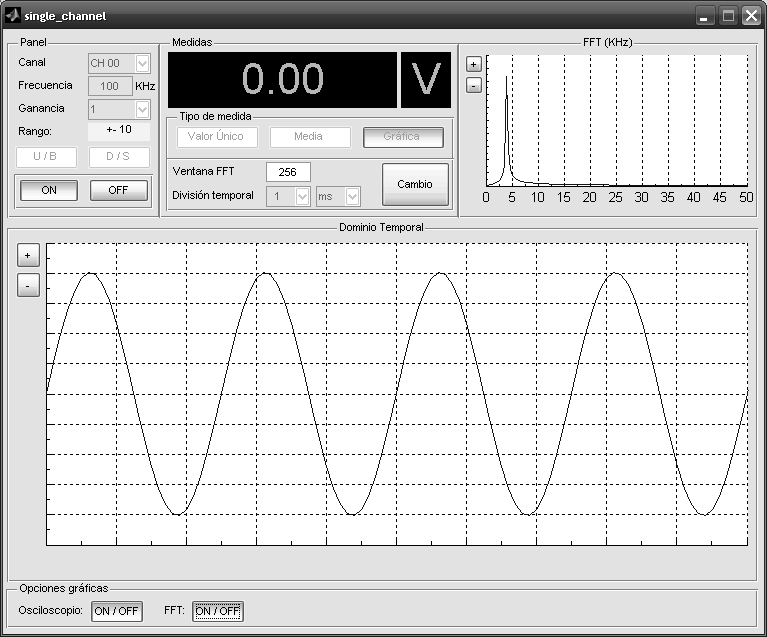
\includegraphics{gis-pfc-appa-01.png}
	\end{center}
	\caption[Aspecto de la interfaz con controles y gr�ficos separados por paneles]{Aspecto de la interfaz con controles y gr�ficos separados por paneles.}
	\label{fig:interface}
\end{figure}

A continuaci�n pueden observarse dos paneles que contienen los espacios de coordenadas destinados a alojar las representaciones de se�al y espectro y varios grupos de controles, uno por cada espacio de coordenadas, cada uno de los cuales controla propiedades del espacio de coordenadas al que est� sujeto. Por �ltimo, un quinto panel dispone de los mandos necesarios para habilitar o deshabilitar la representaci�n de se�al, espectro o ambos.


\section{Especificaciones t�cnicas y limitaciones}

A continuaci�n se enumeran brevemente los requisitos necesarios para poder emplear la aplicaci�n de control.

\begin{itemize}
	\item En primer lugar es necesario un \textsc{pc} funcionando sobre el sistema operativo Microsoft Windows.
	\item En dicho \textsc{pc} debe encontrarse correctamente instalada una tarjeta \kpci{} o similar. Son compatibles con la aplicaci�n las tarjetas fabricadas por \emph{Keithley} que dispongan al menos de un puerto de adquisici�n anal�gica, cuyas caracter�sticas sean similares a la \kpci{} y cuya interacci�n con la \datx{} de \matlab{} sea similar a la interacci�n que se da entre este software y la \kpci{}. Para que una tarjeta de adquisici�n de datos se encuentre correctamente instalada en un \textsc{pc}, en primer lugar debe encontrarse correctamente conectada a la placa base del \textsc{pc} y, en segundo lugar, deben haberse instalado con �xito los drivers de la misma.
	\item Para poder emplear el software resulta imprescindible que en el \textsc{pc} correspondiente se halle instalada una copia de la suite matem�tica \matlab{} cuya versi�n sea compatible con la aplicaci�n.
	\item Es necesario tener acceso desde \matlab{} a los ficheros correspondientes a la aplicaci�n de control que, como es obvio, tendr�n que haberse instalado previamente en el \textsc{pc}.
	\item Es necesaria una interfaz externa compatible con los conectores mini-\sig{d} de la \kpci{}. Puede emplearse por ejemplo la caja de conexiones descrita en el \vref{subsec:conbox}, en ese caso ser� necesaria al menos una sonda en la que, por lo menos, una de las terminaciones sea compatible con la caja de conexiones.
\end{itemize}

Como indica su t�tulo, este apartado se ha pensado adem�s para indicar las limitaciones que muestra la aplicaci�n de control. Desde el punto de vista de su origen estas limitaciones pueden dividirse en limitaciones derivadas del uso de la \kpci{} y en limitaciones introducidas por la propio software. Para una mayor informaci�n sobre las primeras pueden consultarse las \vrefrange{sec:technical}{subsec:throughput} en el segundo cap�tulo. A destacar el comportamiento del rendimiento de la tarjeta que se ver� reducido seg�n se vayan a�adiendo canales al objeto dispositivo.\par
En cuanto a las limitaciones que introduce el software son las siguientes. Para empezar es destacable el hecho de que �nicamente es posible controlar un canal de muestreo desde la aplicaci�n de control. El canal controlado puede estar asociado a cualquier puerto f�sico de la tarjeta pero s�lo se da acceso a un �nico canal por sesi�n. A esta limitaci�n se debe a�adir que desde el software es imposible crear o eliminar canales u objetos dispositivo de forma manual.\par
Por otro lado se da la incapacidad de modificar desde la utilidad propiedades de la configuraci�n de la tarjeta que no vengan representadas por controles en la interfaz de usuario. Algunos de estos controles se deshabilitan durante la actividad de muestreo, se ha hecho as� para impedir que se altere el valor de par�metros tales como la frecuencia de muestreo en tiempo real. En ocasiones es \matlab{} desde un nivel superior en la jerarqu�a del software el que impide que una de estas propiedades cambie al vuelo, en el resto de casos se ha hecho para evitar problemas de rendimiento experimentados durante pruebas de software.\par


\section{Instrucciones de uso}

El manejo del software de representaci�n de se�ales es relativamente sencillo. Para arrancar el software debe ejecutarse en primer lugar \matlab{}\footnote{Si se necesita m�s informaci�n con respecto al uso de \matlab{}, puede consultarse el manual de instrucciones proporcionado por el desarrollador del software.}. Despu�s debe hacerse una llamada a la aplicaci�n de control, existen tres modos de hacer esto mismo, todos ellos explicados con detalle en el manual de usuario de \matlab{}. En lo fundamental el procedimiento es id�ntico a la llamada a una funci�n implementada en un fichero de c�digo de \matlab{}. De los modos mencionados son interesantes desde la perspectiva que adopta este manual dos de ellos.\par

\begin{itemize}
	\item El primero, quiz�s m�s intuitivo, es el modo gr�fico, que m�s bien es un compendio de las distintas formas de ejecutar un fichero *.m que permite \matlab{}, s�lo que aplicado al c�digo de una aplicaci�n con interfaz de usuario. Para dar un ejemplo, desde el navegador de carpetas de \matlab{} puede hacerse click con el bot�n derecho del rat�n en el fichero *.m asociado al software (fichero \texttt{single\_channel.m}) y seguidamente seleccionar en el desplegable que aparece la opci�n <<ejecutar archivo>>.
	\item Otra forma es la llamada desde la l�nea de comandos. Cercior�ndose de que el directorio actual contiene los ficheros \texttt{single\_channel.m} correspondiente al c�digo y \texttt{single\_channel.fig} correspondiente a la distribuci�n de la interfaz puede escribirse en la l�nea de comandos la orden:

		\begin{lstlisting}[gobble=16]
			[handles = ]single_channel[(opciones)]
		\end{lstlisting}

	Siendo la parte entre corchetes del comando opcional.\par Lo interesante de este m�todo es que permite el acceso a las propiedades internas y objetos de los que hace uso la aplicaci�n de control. De este modo es posible a partir del objeto \texttt{handles} tener acceso, por ejemplo, al objeto dispositivo que controla la tarjeta de adquisici�n de se�ales. Adem�s a trav�s de la llamada por l�nea de comandos es posible pasar argumentos para posibles opciones relacionadas con las interfaces de usuario.
\end{itemize}

De no existir ning�n objeto dispositivo asociado a la \kpci{}, la funci�n de creaci�n presente en la aplicaci�n crea, al iniciarse �sta, un objeto dispositivo asociado a la \kpci{} o cualquier otra tarjeta fabricada por \emph{Keithley} soportada por el software e instalada en el \textsc{pc}. En caso contrario el software hereda uno de los posibles objetos dispositivos existentes a�adiendo un nuevo canal y emite un mensaje de advertencia.\par
Al cerrar la aplicaci�n se detiene el proceso de muestreo y, si el n�mero de canales pertenecientes al objeto dispositivo empleado no ha disminuido, se elimina el canal cuyo orden corresponde al n�mero de canales existentes al lanzar la aplicaci�n m�s uno. Es importante remarcar que en ning�n caso se elimina el objeto dispositivo del que se ha hecho uso, ni siquiera cuando es la aplicaci�n la que lo ha generado. Queda pues en manos del usuario la tarea de destruir cualquier canal creado por la aplicaci�n de control y el objeto dispositivo correspondiente en caso de ser necesario. La forma m�s sencilla de hacerlo es la que se cita a continuaci�n, que tambi�n eliminar� cualquier variable que quedase en el espacio de trabajo de \matlab{} ---para evitarlo debe llamarse a \texttt{clear} utilizando como argumentos, separados por espacios entre ellos y del comando, los nombres de los objetos dispositivos eliminados de la memoria de \matlab{} que queden en el espacio de trabajo---.

\begin{lstlisting}
	delete(daqfind);
	clear;
\end{lstlisting}


\subsection{Descripci�n detallada de la interfaz de usuario}

Aqu�, en este apartado, se muestran los controles y sus funciones para que el usuario pueda comprender su funcionamiento. Para facilitar la b�squeda se ha procedido a agrupar las definiciones empleando como criterio la pertenencia a mismo panel, es decir, todos los controles que aparecen reunidos en un mismo panel en la interfaz de usuario se explican en un mismo cuadro.

\begin{table}
	\centering
	\begin{minipage}{.85\textwidth}
		\begin{description}
			\item[Canal] Determina el puerto f�sico asociado al canal en uso. Se trata de un control desplegable que se expande mostrando todos los puertos seleccionables.
			\item[Frecuencia] Permite ajustar la frecuencia de muestreo. La nueva frecuencia de muestreo se limita de forma autom�tica de modo que se encuentre entre 1 kHz y la m�xima frecuencia de muestreo permitida por la tarjeta.
			\item[Ganancia] Ajusta el rango de amplificaci�n del amplificador de instrumentaci�n integrado en la tarjeta. Esto a su vez condiciona la amplitud de pico m�xima de la se�al que entra a la \kpci{}. �ste es tambi�n un control desplegable y muestra el conjunto de ganancias posibles.
			\item[Rango] Indicador que presenta el rango en el que debe mantenerse la amplitud de la se�al que entra a la tarjeta para que el conversor anal�gico digital no sature dada una configuraci�n de ganancia y m�todo de adquisici�n. Puede consultarse el \vref{tab:acqmodes} al respecto.
			\item[Control u/b] Controla el modo de adquisici�n en el proceso de muestreo. El modo de adquisici�n es en la \datx{} una propiedad del objeto dispositivo y no del canal.
			\item[Control d/s] Permite configurar el modo de terminaci�n correspondiente al canal que se controla. De configurarse como diferencial el listado de canales que muestra el desplegable \textsf{canal} se modifica para concordar con esta configuraci�n.
		\end{description}
	\end{minipage}
	\caption[Descripci�n del primer panel de controles]{Descripci�n del primer panel de controles.}
	\label{tab:first-panel}
\end{table}

El primer panel descrito en el \vref{tab:first-panel} alberga un panel secundario o subpanel en el que se encuentran ubicados dos controles m�s. Estos controles son el control \emph{on} y el control \emph{off} que respectivamente sirven para iniciar o detener el proceso de muestreo.\par
El siguiente panel a la derecha con el nombre de \emph{medidas} muestra un indicador num�rico verde en fondo negro que, una vez activado el proceso de muestreo, si la aplicaci�n se encuentra funcionando en los modos \emph{valor �nico} o \emph{media}, presenta el valor que toma la se�al en cada evento. Adicionalmente puede verse un panel m�s peque�o, \emph{tipo de medidas}, dentro de este panel. Los elementos que incorpora el subpanel tipo de medidas vienen explicados en el \vref{tab:second-panel}.

\begin{table}
	\centering
	\begin{minipage}{.85\textwidth}
		\begin{description}
			\item[Tipo de medidas] Representado por tres botones: \emph{valor �nico}, \emph{media}, y \emph{gr�fica}; de los cuales s�lo uno puede quedar pulsado al mismo tiempo. Gobierna el modo de funcionamiento del software de control. Los modos de funcionamiento de la aplicaci�n de control se encuentran explicados al detalle en el \vref{subsec:working-modes}.
			\item[Ventana fft] Determina la longitud en n�mero de muestras de la ventana empleada para el c�lculo de la \textsc{fft}. Este control se presenta en la forma de cuadro de texto editable. El valor introducido en el texto es redondeado a la siguiente potencia de dos.
			\item[Divisi�n temporal] Este mando est� formado por dos controles desplegables. El primero de los cuales permite seleccionar un n�mero de una secuencia que va de 1 a 400. El segundo por su parte sirve para seleccionar una escala de unidades: milisegundos o microsegundos. El prop�sito del conjunto es controlar la longitud temporal que representa el eje de coordenadas del espacio de coordenadas en el que se representa la se�al. Esto que a priori parece no repercutir demasiado en el funcionamiento del software, adquiere una gran importancia dado que el software de control se ha dise�ado para asemejarse en su modo de funcionamiento gr�fico a un osciloscopio digital. Para m�s informaci�n sobre el funcionamiento de los osciloscopios digitales cons�ltese el \vref{subsec:repmodes}.
			\item[Cambio] Inicialmente la \textsc{fft} de la se�al se representa en el espacio de coordenadas m�s peque�o, arriba a la derecha en la interfaz de usuario, y la se�al se representa en el espacio de coordenadas mayor. Mediante este mando es posible reubicar las representaciones de se�al y transformada de Fourier.
		\end{description}
	\end{minipage}
	\caption[Descripci�n del segundo panel de controles]{Descripci�n del segundo panel de controles incluido en el panel \emph{medidas}.}
	\label{tab:second-panel}
\end{table}

Para terminar existe un panel adicional que incorpora los controles \emph{osciloscopio} y \emph{fft}. Sendos mandos permiten en el modo de funcionamiento gr�fico habilitar o inhabilitar la representaci�n de la se�al y/o el c�lculo y representaci�n de la \textsc{fft} de la se�al respectivamente. Asimismo, cada uno de los paneles en los que se sit�an los espacios de coordenadas est� dotado de dos controles con una etiqueta que representa los signos matem�ticos de la suma y la resta. Estos botones controlan la escala axial en relaci�n con el eje de ordenadas en el espacio de coordenadas al que acompa�an.


\subsection{Modos de funcionamiento}\label{subsec:working-modes}

Los modos de funcionamiento que soporta el software de control de la \kpci{} son tres. En el �ltimo de ellos, el modo gr�fico, la aplicaci�n consigue simular un osciloscopio digital de acuerdo con los resultados mostrados en la \vref{sec:working-test}. Se han discutido los pormenores de este modo de funcionamiento a lo largo del grueso de la memoria, para evitar reiteraciones innecesarias no volver� a tratarse el tema en este punto.\par
El resto de modos de funcionamiento podr�a catalogarse como modos num�ricos o no gr�ficos. La raz�n es que durante el proceso de adquisici�n el usuario percibe un valor num�rico y no una representaci�n gr�fica de la se�al si alguno de estos modos se encuentra activado. Es importante destacar que estos modos de funcionamiento no son apropiados para el estudio de se�ales de alta frecuencia. En situaciones en las que la se�al oscila a alta frecuencia el an�lisis mediante la aplicaci�n configurada para funcionar en alguno de estos dos modos aporta informaci�n confusa que no debe ser tomada en cuenta. No obstante, se recomienda encarecidamente su uso de producirse la situaci�n contraria, aquella en la que la se�al analizada oscila con lentitud. Esto es debido en principio a la naturaleza de los algoritmos en los que se basan ambos modos de funcionamiento y los resultados que otorgan.\par % en cuanto a que aportan en tales circunstancias / en tal caso informaci�n confusa acerca de la se�al / se�ales / informaci�n no representativa.
Los modos num�ricos de funcionamiento comparten una mec�nica similar, en lo fundamental id�ntica, no obstante, diferente en cuanto a implementaci�n. La idea es programar, antes de que d� inicio el proceso de adquisici�n, los eventos relacionados con el objeto dispositivo de la \datx{} de modo que ocurran peri�dicamente. Cuando acontece uno de los eventos se obtiene un n�mero real a partir de una interpretaci�n hecha a partir de la muestra o muestras adquiridas desde el evento anterior y se escribe �ste en el indicador num�rico que forma parte de la interfaz de usuario. Hasta ah� las coincidencias entre los m�todos que ejecuta cada modo de funcionamiento.\par % de modo cada cierto n�mero peri�dico de muestras obtenidas se programan
Las diferencias entre el m�todo \emph{valor �nico} y \emph{media} son las que siguen:

\begin{itemize}
	% \item En primer lugar, con el modo valor �nico se obtiene el valor de la muestra adquirida justo antes, despu�s de producirse el evento, mientras que el modo media proporciona la media aritm�tica de las muestras obtenidas desde el evento inmediatamente anterior al actual al ritmo especificado por el control \textsf{frecuencia}.
	\item En primer lugar, en el modo valor �nico el software muestra en el display\footnote{A partir de la vig�simo tercera edici�n del diccionario de la real academia de la lengua se considera correcto decir visualizador e incorrecto decir \emph{display}.} el valor correspondiente a la muestra obtenida justo despu�s de producirse el �ltimo evento, mientras que el modo media proporciona la media aritm�tica de las muestras obtenidas desde el evento inmediatamente anterior al actual al ritmo especificado por el control \textsf{frecuencia}.
	\item M�s all� de lo inferido a partir del nombre de los modos, estos se diferencian en el criterio empleado en la definici�n del periodo entre eventos y en la herramienta que genera dichos eventos. El m�todo valor �nico emplea el reloj interno de la \kpci{} a modo de temporizador, los eventos en este modo se programan para que sucedan cada cuarto de segundo. Por el contrario el modo media emplea una especie de testigo electr�nico que implementa la \datx{} y que produce un evento cada vez que se adquiere un determinado n�mero de muestras definido por el usuario de \matlab{}, en este caso el programador, a trav�s de la propiedad \textsf{SamplesAcquiredFcnCount}. El n�mero de muestras que debe adquirirse antes de que se produzca un evento se ha configurado a un valor que queda entre la cantidad de muestras que se obtienen en 250 milisegundos a la frecuencia de muestreo establecida y un m�nimo que \matlab{} actualiza al modificarse esta frecuencia.
	\item Por �ltimo, cabe hacer menci�n al procedimiento empleado para obtener el valor que se muestra por pantalla. El modo valor �nico emplea la funci�n \texttt{getsample} que extrae una �nica muestra de la tarjeta de adquisici�n, de este forma la tarjeta pasa gran parte del periodo entre eventos en reposo. El modo media, por el contrario, utiliza la funci�n \texttt{mean} sobre \texttt{getdata} que recupera las muestras almacenadas hasta el momento en el buffer en tanto que lo borra.
\end{itemize}


\subsubsection[Modos num�ricos y se�ales de alta frecuencia]{Incompatibilidades entre los modos de funcionamiento num�ricos y el an�lisis de se�ales de alta frecuencia}

La raz�n de que estos modos de funcionamiento no sean apropiados para el estudio de se�ales de alta frecuencia es diferente seg�n el modo.

\begin{itemize}
	% \item El modo valor �nico extrae una muestra de la se�al de manera peri�dica. Si consideramos que la se�al resultante de este proceso es el producto entre la se�al analizada y un tren de deltas. Si combinamos el hecho de que la frecuencia de la se�al es superior o muy superior a la frecuencia del tren de deltas y que posiblemente no sea un m�ltiplo de �sta con la certeza de que ambas se�ales se encuentran desfasadas en una medida desconocida y que es dif�cil seguir un n�mero real que cambia cuatro veces por segundo, el resultado es una informaci�n ca�tica y poco representativa de la se�al.  % Dependiente del modo pero radica en la forma de obtener el n�mero que se muestra por pantalla. El primer m�todo aplicado a una se�al que oscila no en fase con la se�al de muestreo hace parecer el comportamiento de la se�al err�tico. El segundo, la media de muchos periodos de una se�al centrada en el origen tiende a cero.
	\item El modo valor �nico extrae una muestra de la se�al de manera peri�dica, con un periodo de un cuarto de segundo. Es decir, se muestrea la se�al a una frecuencia de muestreo de 4 Hz. Considerando la condici�n de que la frecuencia de la se�al muestreada es muy alta, puede considerarse como consecuencia la hip�tesis de que sea muy superior a la frecuencia de muestreo, adem�s es poco probable que la primera sea un m�ltiplo de la segunda. Si se combina esta suposici�n con la certeza de que el instante en el que empieza el muestreo no coincide con el instante en el que se origina la se�al, puede llegarse a la conclusi�n de que la informaci�n presentada en el visor es, empleando el modo valor �nico en el an�lisis de se�ales r�pidas, ca�tica, cuanto menos confusa y poco representativa de la se�al. % ambas frecuencias pueden no estar relacionadas por una raz�n de multiplicidad. Si combinamos el hecho de que la frecuencia de la se�al muestreada es muy superior a la frecuencia de muestreo, con la posibilidad probable de que la frecuencia de la se�al no sea un m�ltiplo de la frecuencia de muestreo, con la certeza de que el instante en el que empieza el muestreo no coincide con el instante en el que se origina la se�al.
	\item En el caso del modo media ocurre que la media de una cantidad determinada de periodos de una se�al peri�dica tiende m�s a cero cuanto m�s periodos de la se�al se estiman al calcular la media. Por tanto, si la frecuencia de la se�al es mucho mayor que la frecuencia con la que se actualiza el valor num�rico mostrado por pantalla, y �sta tambi�n est� en torno a 4 Hz, el valor que se obtiene es el cero.
\end{itemize}

No es que el modo de funcionamiento gr�fico de la aplicaci�n de control carezca de utilidad en el an�lisis de se�ales de baja frecuencia, si no que carece de utilidad pr�ctica. Debe recordarse al lector que el modo de funcionamiento gr�fico de la aplicaci�n sobre la que trata este manual pretende emular un osciloscopio digital en su modo de funcionamiento gr�fico y, como consecuencia, este modo de funcionar adolece de los problemas propios de este tipo dispositivos como por ejemplo el que se expone en este p�rrafo. El modo de representaci�n que adopta un osciloscopio digital para representar se�ales lentas es el modo de representaci�n continuo, dada la incapacidad de la funci�n de disparo del modo convencional de trabajar con este tipo de se�ales \footnote{Esto queda suficientemente explicado en el \vref{subsec:repmodes}.}. Este modo no aporta informaci�n visual precisa sobre la frecuencia de la se�al analizada ni sobre su valor de pico a pico. Por si fuera poco dada la implementaci�n que se le ha dado en esta aplicaci�n consume muchos m�s recursos que el modo de representaci�n convencional\footnote{De hecho en las pruebas de software que se han realizado para este proyecto el modo de representaci�n continuo no funciona excepto en el modo de depuraci�n de errores pausando la ejecuci�n del software, si bien es cierto las pruebas se realizaron con un \textsc{pc} poco actualizado.}. Y, como es obvio, el modo gr�fico independientemente del modo de representaci�n adoptado necesita m�s recursos de los que requieren el resto de modos de funcionamiento.\par
Es por esta raz�n por la que los modos num�ricos obtienen un mayor protagonismo en el an�lisis de se�ales de baja frecuencia, porque aportan una informaci�n lo bastante buena, comparable a la que proporciona el modo gr�fico, y consumen menos recursos que esta alternativa.


\addtocounter{totalpages}{\value{page}}
\addtocounter{totalpages}{-1}
\setcounter{page}{1}
\chapter{Pruebas y contenidos adicionales}

Este apéndice no debe adjuntarse en el documento final, en el se anotarán
ideas para modificar el contenido del grueso del documento y bases para
generar los contenidos adicionales.


\section{Configuración de página}

La configuración actual se ha hecho utilizando el paquete \textsf{typearea}
que forma parte del conjunto del \textsc{koma}-\textsc{s}cript. Las
opciones más importantes que deben pasarse a este paquete son el tipo de
papel (A4, A3, A5, letter,\dots) y el espacio de corrección necesario para
evitar fallos en la encuadernación (\textsc{bcor} = \texttt{magnitud} o
directamente \textsc{bcor}\texttt{magnitud}). Utilizando el paquete
\textsf{layouts} pueden crearse figuras que representen la configuración de
página actual.

\newlength{\auxmm}
\newlength{\auxin}
\newlength{\auxpt}
\setlength{\auxmm}{1mm}
\setlength{\auxin}{1in}
\setlength{\auxpt}{1pt}
\newsavebox\caja
\sbox\caja{\includegraphics{gis-pfc-ch2-02.mps}}

\begin{table}
	\centering
	\printinunitsof{mm}\pagevalues\medskip\par

	\begin{tabular}{l l}
		\toprule
		1in = \printinunitsof{mm}\prntlen{\auxin} %
		& 1pt = \printinunitsof{mm}\prntlen{\auxpt} \\
		1mm = \printinunitsof{in}\prntlen{\auxmm} %
		& 1mm = \printinunitsof{pt}\prntlen{\auxmm} \\
		Alto de \texttt{gis-ch2-02.mps} %
		& \printinunitsof{mm}\prntlen{\ht\caja} \\
		Ancho de \texttt{gis-ch2-02.mps} %
		& \printinunitsof{mm}\prntlen{\wd\caja} \\
		marginparwidth %
		= \printinunitsof{pt}\prntlen{\marginparwidth} %
		& marginparsep %
		= \printinunitsof{pt}\prntlen{\marginparsep} \\
		\bottomrule
	\end{tabular}
	\caption[Valores actuales de la distribución de página]{Valores que
	completan el diagrama representado en la \vref{fig:layouts}
	sustituir la nomenclatura de referencia por los valores
	correspondientes}
\end{table}

\begin{figure}
	\begin{center}
		\includegraphics{gis-pfc-ch2-02.mps}
	\end{center}
	\caption[Segunda figura del segundo capítulo]{Segunda figura del
	segundo capítulo.}
	\label{fig:ch102}
\end{figure}

El lector puede fijarse que se cumple la regla de construcción que aplica
el paquete \textsf{typearea} en la que el margen inferior es dos veces el
margen inferior, y que el margen interior de página ---una vez eliminado el
centímetro (\textsc{bcor}\texttt{1cm}) que se deja para compensar el
encuadernado--- es la mitad del margen exterior de página. De ese modo se
crea una distribución de página en la que el margen interior de página de
las páginas par e impar juntas es igual a cada uno de los márgenes
exteriores de ambas páginas.

\begin{figure}
	\pagediagram
	\caption{Distribución del texto en las páginas de este documento}
	\label{fig:layouts}
\end{figure}

\begin{figure}\ContinuedFloat
	\currentpage
	\pagedesign
	\caption[]{Continuación del \vref{fig:layouts}}
\end{figure}


\section{Gráficos con MetaPost}

Anotaciones destinadas a obtener gráficos escalables de calidad empleando
el paquete MetaPost para la creación de gráficos en PostScript.


\subsection{Tamaño}

Tengo que modificar el tamaño de algunas figuras al haber cambiado la
tipografía predeterminada de la \emph{Computer Roman} a \emph{Lucida}. Lo
que quiero que aparezca en este apartado es un cuadro con los distintos
tamaños de letra que aparecen en el documento.


\section{Listados}

Estoy modificando las etiquetas que \LaTeX{} utiliza para escribir los
entornos de listados sin número, pongo aquí un ejemplo para ver como va
quedando.

\begin{itemize}
	\item Este es un ítem de primer nivel en un entorno de listado,
		puede observarse la etiqueta de primer nivel.

		\begin{itemize}
			\item Este es un elemento de un listado que
				pertenece al segundo nivel, aquí puede
				observarse la etiqueta perteneciente a
				dicho nivel.
			\item Puedo confirmar que me gusta más la etiqueta
				que he utilizado ahora para el primer nivel
				que la que utilizaba por defecto antes.
		\end{itemize}

\end{itemize}


\backmatter

\addtocounter{totalpages}{\value{page}}
\addtocounter{totalpages}{-1}
\setcounter{page}{\value{totalpages}}
\renewcommand\thepage{\arabic{page}}
\nocite{mittelbach2004lc, stutzman1997atd, garcia2000mrsr}
\bibliographystyle{bababbrv-lf}
\bibliography{gis-pfc}

\end{document}
